To improve the exclusion limit on the \brThb, the \mjj from following 
event categories have been used for limit computation:
\subsection{Inclusive Event Category without charm-jet Tagging}
\label{ss:mjj_Inc}
The \mjj distribution without further categorizing events based on charm 
tagging was used at 8 TeV~\cite{Khachatryan:2015uua} for limit computation due 
to the unavailability of dedicated charm taggers. For sake of comparison, at 
13 TeV also the exclusion limit is computed using \mjj after kinematic fit
selection, without the charm tagging. The event yields are shown in Table~
\ref{tab:eventYieldInc}. Corresponding \mjj distributions are shown in 
Figures~\ref{subfig:mjj_kfit_muKinFit},~\ref{subfig:mjj_kfit_eleKinFit}, 
~\ref{subfig:mjj_sig_kfit_mu},~\ref{subfig:mjj_sig_kfit_ele}. The corresponding 
systematics and statistical uncertainties from different sources are shown in 
Table~\ref{tab:sysInc}. The exclusion limit for inclusive event category is 
computed in Sec.~\ref{ss:limit_Inc}. 
\begin{table}
\caption{Event yield for inclusive category.}
\label{tab:eventYieldInc}
\begin{center}
\begin{tabular}{cccc}
\hline 
\hline 
\bf{Process}& $N_{events} \pm stat \pm sys$ & $N_{events} \pm stat \pm sys$\\ 
 & $\mu$ + jets &  e + jets\\
\hline 
\hline 
$m_{\PSHp}=80$  \GeV & 16719 $\pm$ 114 $\pm$ 778 & 11842 $\pm$ 94 $\pm$ 539\\
$m_{\PSHp}=90$  \GeV & 16891 $\pm$ 113 $\pm$ 789 & 12197 $\pm$ 95 $\pm$ 594\\
$m_{\PSHp}=100$ \GeV & 17548 $\pm$ 115 $\pm$ 857 & 12339 $\pm$ 95 $\pm$ 548\\
$m_{\PSHp}=120$ \GeV & 16932 $\pm$ 113 $\pm$ 787 & 11959 $\pm$ 94 $\pm$ 547\\
$m_{\PSHp}=140$ \GeV & 13404 $\pm$ 101 $\pm$ 680 & 9570 $\pm$ 84 $\pm$ 503\\
$m_{\PSHp}=150$ \GeV & 9579 $\pm$ 85 $\pm$ 552 & 6948 $\pm$ 71 $\pm$ 421\\
$m_{\PSHp}=155$ \GeV & 7562 $\pm$ 77 $\pm$ 458 & 5464 $\pm$ 65 $\pm$ 371\\
$m_{\PSHp}=160$ \GeV & 5767 $\pm$ 66 $\pm$ 383 & 4225 $\pm$ 56 $\pm$ 289\\
SM $t\bar{t}$ + jets & 205677 $\pm$ 278 $\pm$ 9885 & 143178 $\pm$ 228 $\pm$ 7200\\
Single ~t & 5739 $\pm$ 30 $\pm$ 339 & 4030 $\pm$ 25 $\pm$ 244\\
QCD multijet & 1104 $\pm$ 117 $\pm$ 0 & 4308 $\pm$ 192 $\pm$ 0\\
W + jets & 2979 $\pm$ 86 $\pm$ 450 & 2115 $\pm$ 72 $\pm$ 173\\
$Z/\gamma$ + jets & 441 $\pm$ 17 $\pm$ 45 & 453 $\pm$ 15 $\pm$ 47\\
VV & 156 $\pm$ 21 $\pm$ 16 & 67 $\pm$ 13 $\pm$ 13\\
All background & 216096 $\pm$ 316 $\pm$ 10593 & 154153 $\pm$ 309 $\pm$ 7604\\
Data & 203178 $\pm$ 451 & 148499 $\pm$ 385 \\
\hline 
\end{tabular}
\end{center}
\end{table}

\begin{table}
\caption{Systematic and statistical uncertainties in \%,  from inclusive 
    category for muon (electron) channel. The "---" indicates that the 
    corresponding uncertainties are not considered for the given process.}
\label{tab:sysInc}
\centering
\begin{adjustbox}{max width=\textwidth}
\begin{tabular}{  c c c c c c c c c c c c c cc}
\hline 
\hline 
Process &{\rotatebox{90}{Luminosity}} & {\rotatebox{90}{Pileup} } & {\rotatebox{90}{Lepton }} & {\rotatebox{90}{JES + JER + \MET}} & { \rotatebox{90}{b \& c-jet tagging-1} }  & { \rotatebox{90}{b \& c-jet tagging-2} } & { \rotatebox{90}{b \& c-jet tagging-3}}& { \rotatebox{90}{Normalization}  }& {\rotatebox{90}{Statistical}  } & {\rotatebox{90}{top \pt } }  \\ 
\hline 
\hline 
$m_{H^+}=80$ GeV & 2.5 (2.5) &  0.8 (0.9) &  3.0 (3.0) & 3.3 (3.1) &  0.0 (0.0) &  0.3 (0.3) &  3.2 (3.2) &  6.1 (6.1) & 0.7 (0.8) & 1.6 (1.9) \\ 
$m_{H^+}=90$ GeV & 2.5 (2.5) &  0.6 (0.8) &  3.0 (3.0) & 3.3 (3.5) &  0.0 (0.0) &  0.3 (0.3) &  3.2 (3.2) &  6.1 (6.1) & 0.7 (0.8) & 1.5 (2.1) \\ 
$m_{H^+}=100$ GeV & 2.5 (2.5) &  0.7 (0.8) &  3.0 (3.0) & 3.6 (2.9) &  0.0 (0.0) &  0.3 (0.3) &  3.2 (3.2) &  6.1 (6.1) & 0.7 (0.8) & 1.5 (1.9) \\ 
$m_{H^+}=120$ GeV & 2.5 (2.5) &  0.6 (1.1) &  3.0 (3.0) & 3.2 (3.0) &  0.0 (0.0) &  0.3 (0.3) &  3.3 (3.3) &  6.1 (6.1) & 0.7 (0.8) & 1.5 (1.9) \\ 
$m_{H^+}=140$ GeV & 2.5 (2.5) &  0.8 (1.0) &  3.0 (3.0) & 3.5 (3.8) &  0.0 (0.0) &  0.4 (0.4) &  3.5 (3.5) &  6.1 (6.1) & 0.8 (0.9) & 2.1 (2.4) \\ 
$m_{H^+}=150$ GeV & 2.5 (2.5) &  0.6 (0.9) &  3.0 (3.0) & 4.3 (4.6) &  0.0 (0.0) &  0.6 (0.6) &  3.8 (3.7) &  6.1 (6.1) & 0.9 (1.0) & 2.6 (3.3) \\ 
$m_{H^+}=155$ GeV & 2.5 (2.5) &  0.5 (0.6) &  3.0 (3.0) & 4.6 (5.5) &  0.0 (0.0) &  0.8 (0.7) &  3.8 (3.9) &  6.1 (6.1) & 1.0 (1.2) & 3.2 (3.5) \\ 
$m_{H^+}=160$ GeV & 2.5 (2.5) &  0.1 (0.8) &  3.0 (3.0) & 5.2 (5.5) &  0.0 (0.0) &  0.9 (1.0) &  4.0 (3.9) &  6.1 (6.1) & 1.1 (1.3) & 3.4 (3.7) \\ 
\hline 
$t\bar{t} + jets$ & 2.5 (2.5) &  0.7 (0.8) &  3.0 (3.0) & 3.3 (3.3) &  0.0 (0.0) &  0.3 (0.3) &  3.1 (3.1) &  6.1 (6.1) & 0.1 (0.2) & 1.5 (2.0) \\ 
Single ~t & 2.5 (2.5) &  0.3 (0.5) &  3.0 (3.0) & 4.7 (4.9) &  0.0 (0.0) &  0.7 (0.7) &  3.5 (3.5) &  5.0 (5.0) & 0.5 (0.6) & --- \\ 
W+jets & 2.5 (2.5) &  2.4 (0.6) &  3.0 (3.0) & 13.6 (5.9) &  0.0 (0.0) &  4.3 (3.8) &  4.2 (4.2) &  5.0 (5.0) & 2.9 (3.4) & --- \\ 
$Z/\gamma$ + jets & 2.5 (2.5) &  1.9 (2.8) &  3.0 (3.0) & 8.6 (8.7) &  0.0 (0.0) &  3.8 (3.2) &  3.5 (3.7) &  4.5 (4.5) & 3.9 (3.4) & --- \\ 
VV & 2.5 (2.5) &  0.9 (4.9) &  3.0 (3.0) & 9.0 (17.9) &  0.0 (0.0) &  1.7 (1.3) &  4.9 (3.3) &  4.0 (4.0) & 13.2 (18.9) & --- \\ 
QCD multijet & --- &  --- &  --- & --- &  --- &  --- &  --- &  10(10) & 10.6 (4.5) & --- \\ 
\hline 
\end{tabular}
\end{adjustbox}
\end{table}
    
\subsection{Inclusive Event Category with Loose charm-jet Tagging}
\label{ss:mjj_cTagL}
The charm taggers as discussed in Sec.~\ref{s:cTag} are used to tag a jet 
as c-jet. One of the jets forming \mjj is required to pass the charm-tagging
requirement. The event yields for loose charm working points after applying 
c-tag event weights are shown in Table~\ref{tab:eventYieldCTagInc}. The 
\mjj distribution with inclusive loose charm tagging working points are 
shown in Figure~\ref{fig:mjj_cTagL}. The corresponding systematics and statistical 
uncertainties from different sources are shown in Table~\ref{tab:sysCTagInc}. 
Exclusion limits using \mjj after applying loose charm tagging is computed 
in Sec.~\ref{ss:limit_cTagL}.
    \begin{figure}
    \centering  
    \subfigure[\mjj for loose WP. \label{subfig:mjj_kfit_CTagIncL_muKinFit}]
    {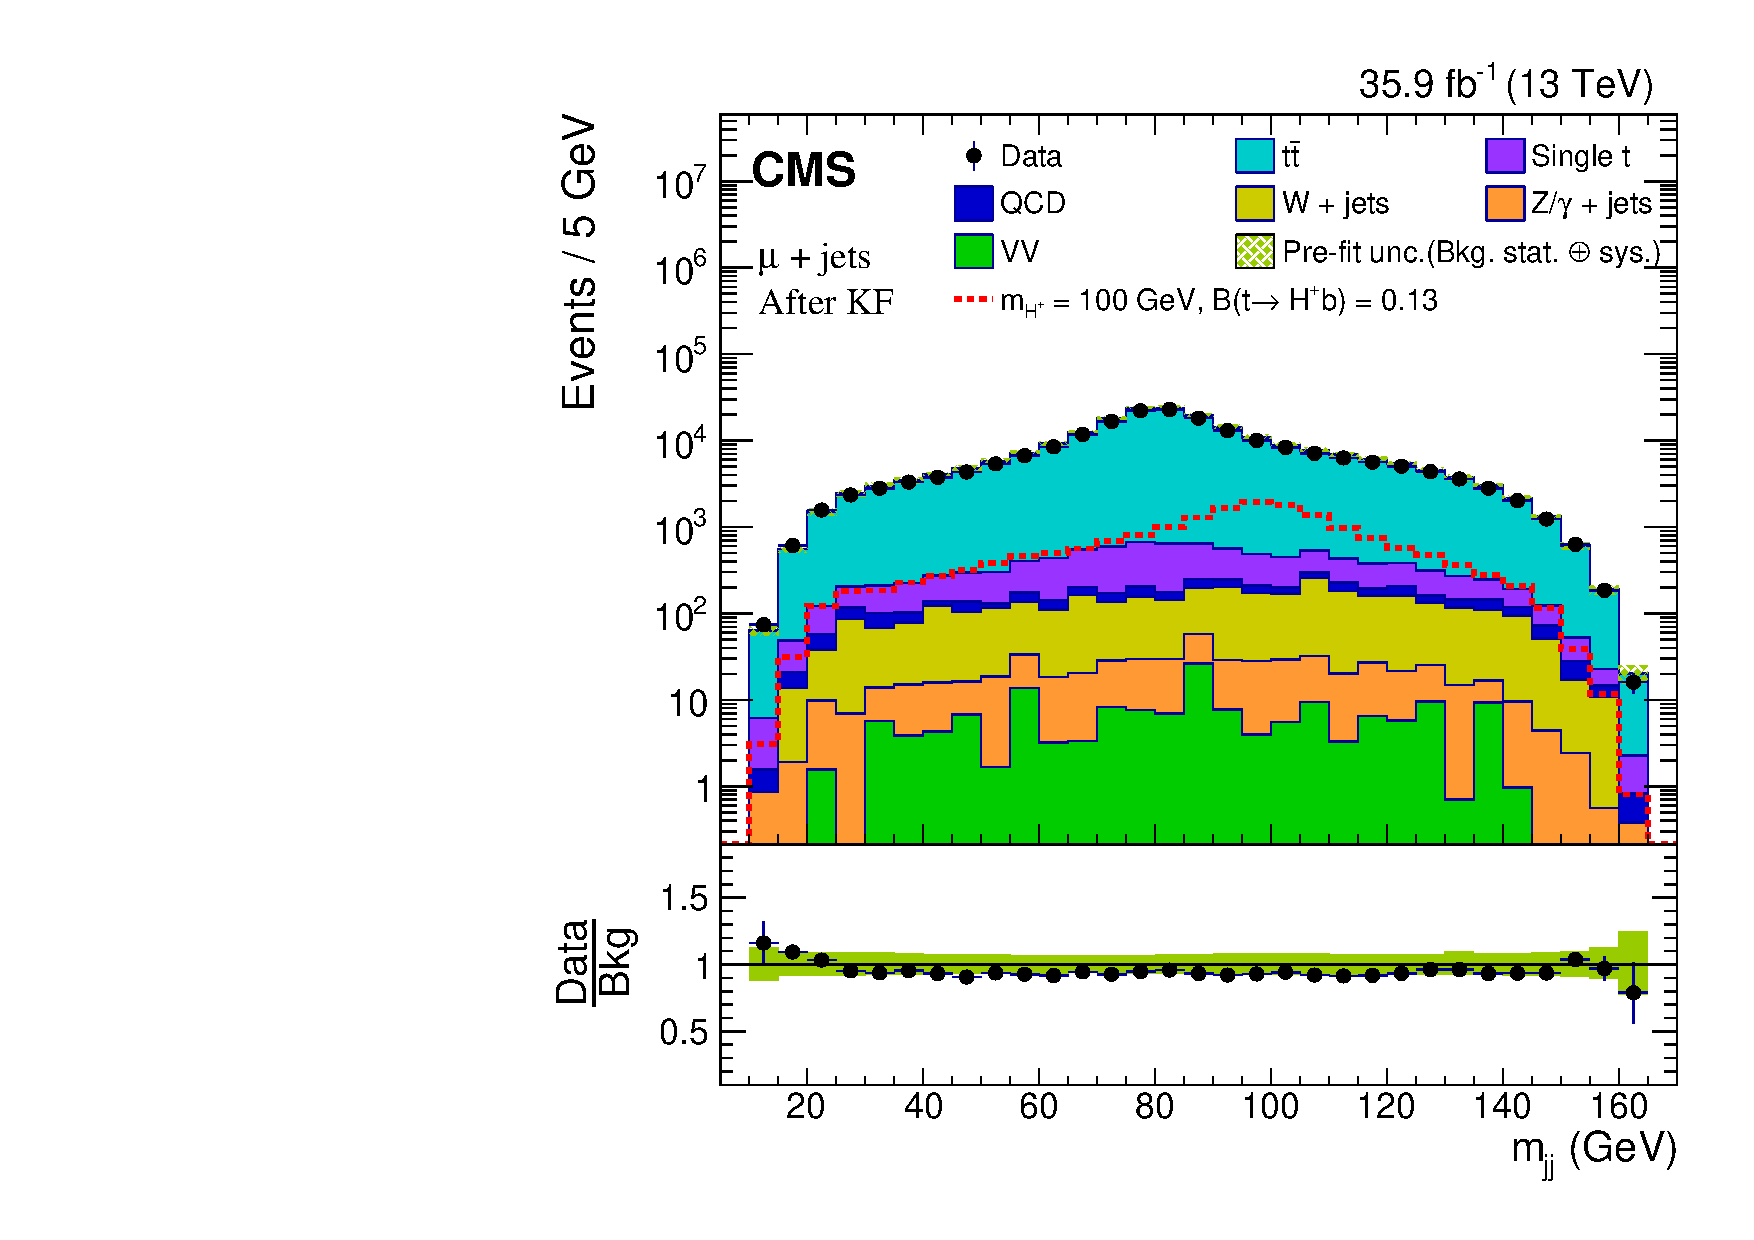
\includegraphics[width=0.45\linewidth]{Image/Muon/KinFit/mjj_kfit_CTagIncL_muKinFit.pdf}}
    \subfigure[\mjj for loose WP.\label{subfig:mjj_kfit_CTagIncL_eleKinFit}]
    {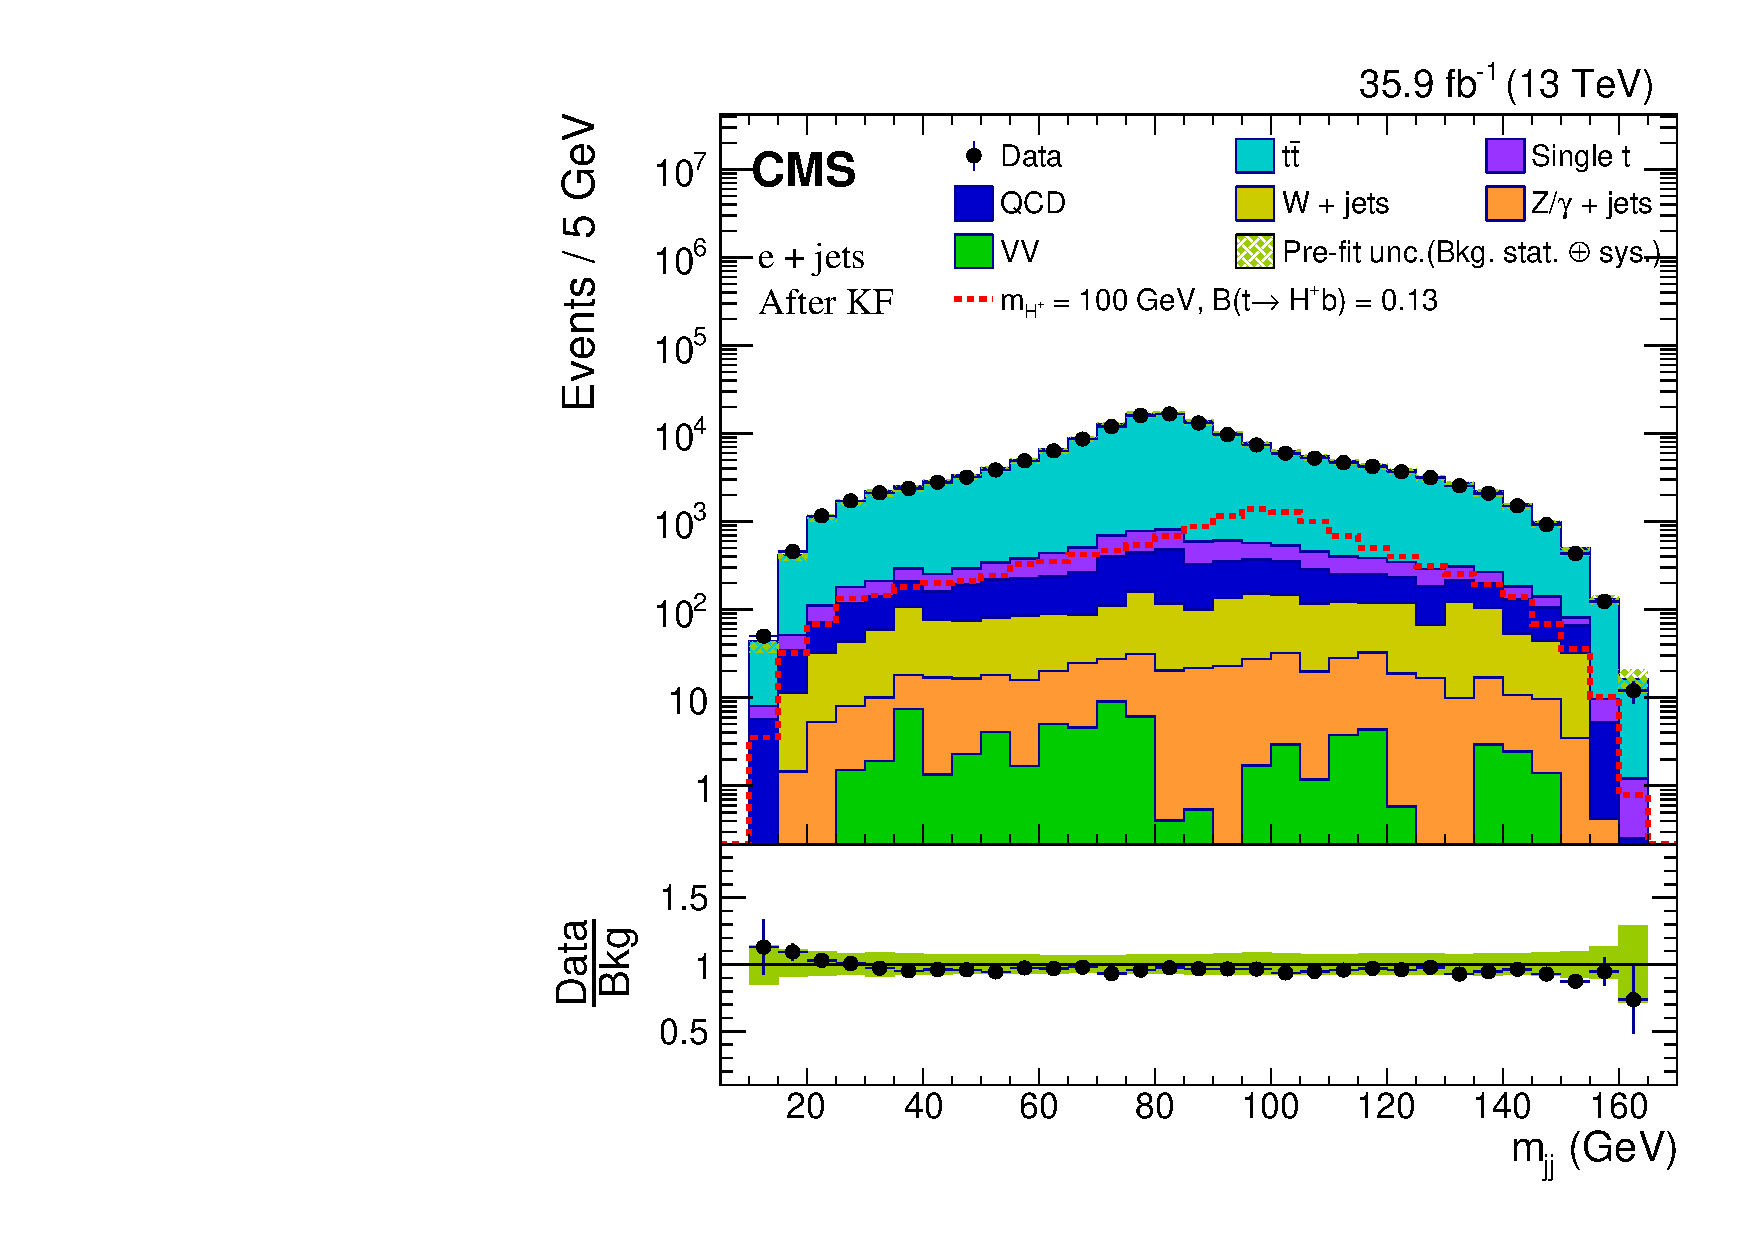
\includegraphics[width=0.45\linewidth]{Image/Electron/KinFit/mjj_kfit_CTagIncL_eleKinFit.pdf}}
    \caption{Distribution of \mjj for inclusive loose charm working point as
    described in Sec.~\ref{ss:mjj_cTagL} for \mujets and \ejets channel.}
    \label{fig:mjj_cTagL}
    \end{figure}
\begin{table}
\caption{Event yield for inclusive loose charm category.}
\label{tab:eventYieldCTagInc}
\begin{center}
\begin{tabular}{cccc}
\hline 
\hline 
\bf{Process}& $N_{events} \pm stat \pm sys$ & $N_{events} \pm stat \pm sys$\\
 & $\mu$ + jets &  e + jets\\
\hline 
\hline 
$m_{\PSHp}=80$ \GeV & 16742 $\pm$ 114 $\pm$ 1191 & 11851 $\pm$ 95 $\pm$ 830\\
$m_{\PSHp}=90$ \GeV & 16906 $\pm$ 114 $\pm$ 1202 & 12193 $\pm$ 96 $\pm$ 886\\
$m_{\PSHp}=100$ \GeV & 17593 $\pm$ 116 $\pm$ 1285 & 12362 $\pm$ 96 $\pm$ 868\\
$m_{\PSHp}=120$ \GeV & 16995 $\pm$ 114 $\pm$ 1247 & 11989 $\pm$ 95 $\pm$ 873\\
$m_{\PSHp}=140$ \GeV & 13466 $\pm$ 102 $\pm$ 1062 & 9618 $\pm$ 85 $\pm$ 767\\
$m_{\PSHp}=150$ \GeV & 9628 $\pm$ 86 $\pm$ 828 & 6980 $\pm$ 72 $\pm$ 618\\
$m_{\PSHp}=155$ \GeV & 7609 $\pm$ 78 $\pm$ 697 & 5498 $\pm$ 65 $\pm$ 521\\
$m_{\PSHp}=160$ \GeV & 5790 $\pm$ 67 $\pm$ 556 & 4245 $\pm$ 57 $\pm$ 416\\
SM $t\bar{t}$ + jets & 204576 $\pm$ 278 $\pm$ 14666 & 142431 $\pm$ 229 $\pm$ 10408\\
Single ~t & 5693 $\pm$ 30 $\pm$ 472 & 3995 $\pm$ 25 $\pm$ 338\\
QCD multijet & 887 $\pm$ 110 $\pm$ 0 & 3993 $\pm$ 185 $\pm$ 0\\
W + jets & 2932 $\pm$ 86 $\pm$ 522 & 2074 $\pm$ 72 $\pm$ 251\\
$Z/\gamma$ + jets & 423 $\pm$ 16 $\pm$ 55 & 439 $\pm$ 15 $\pm$ 57\\
VV & 156 $\pm$ 21 $\pm$ 19 & 67 $\pm$ 13 $\pm$ 13\\
All background & 214667 $\pm$ 314 $\pm$ 15619 & 153000 $\pm$ 305 $\pm$ 11022\\
Data & 201331 $\pm$ 449 & 147210 $\pm$ 384 \\
\hline 
\end{tabular}
\end{center}
\end{table}

\begin{table}
\caption{Systematic and statistical uncertainties in \%, from inclusive loose 
charm-category for muon (electron) channel. The "---" indicates that the 
corresponding uncertainties are not considered for the given process.}
\label{tab:sysCTagInc}
\centering
\begin{adjustbox}{max width=\textwidth}
\begin{tabular}{  c c c c c c c c c c c c c cc}
\hline 
\hline 
Process &{\rotatebox{90}{Luminosity}} & {\rotatebox{90}{Pileup} } & {\rotatebox{90}{Lepton }} & {\rotatebox{90}{JES + JER + \MET}} & { \rotatebox{90}{b \& c-jet tagging-1} }  & { \rotatebox{90}{b \& c-jet tagging-2} } & { \rotatebox{90}{b \& c-jet tagging-3}}& { \rotatebox{90}{Normalization}  }& {\rotatebox{90}{Statistical}  } & {\rotatebox{90}{top \pt } }  \\ 
\hline 
\hline 
$m_{H^+}=80$ GeV & 2.5 (2.5) &  0.8 (0.9) &  3.0 (3.0) & 3.3 (3.0) &  1.4 (1.4) &  4.0 (4.0) &  4.6 (4.6) &  6.1 (6.1) & 0.7 (0.8) & 1.6 (1.9) \\ 
$m_{H^+}=90$ GeV & 2.5 (2.5) &  0.6 (0.8) &  3.0 (3.0) & 3.3 (3.6) &  1.3 (1.3) &  4.0 (4.0) &  4.6 (4.6) &  6.1 (6.1) & 0.7 (0.8) & 1.5 (2.1) \\ 
$m_{H^+}=100$ GeV & 2.5 (2.5) &  0.7 (0.8) &  3.0 (3.0) & 3.5 (2.8) &  1.3 (1.3) &  4.0 (4.0) &  4.8 (4.8) &  6.1 (6.1) & 0.7 (0.8) & 1.5 (1.9) \\ 
$m_{H^+}=120$ GeV & 2.5 (2.5) &  0.6 (1.1) &  3.0 (3.0) & 3.2 (3.0) &  1.2 (1.3) &  4.0 (4.0) &  5.1 (5.0) &  6.1 (6.1) & 0.7 (0.8) & 1.5 (1.9) \\ 
$m_{H^+}=140$ GeV & 2.5 (2.5) &  0.8 (1.0) &  3.0 (3.0) & 3.5 (3.8) &  1.2 (1.2) &  4.1 (4.1) &  5.6 (5.5) &  6.1 (6.1) & 0.8 (0.9) & 2.1 (2.4) \\ 
$m_{H^+}=150$ GeV & 2.5 (2.5) &  0.6 (0.9) &  3.0 (3.0) & 4.3 (4.7) &  1.1 (1.2) &  4.4 (4.4) &  5.9 (5.9) &  6.1 (6.1) & 0.9 (1.0) & 2.6 (3.3) \\ 
$m_{H^+}=155$ GeV & 2.5 (2.5) &  0.5 (0.6) &  3.0 (3.0) & 4.7 (5.4) &  1.1 (1.1) &  4.7 (4.7) &  6.2 (6.1) &  6.1 (6.1) & 1.0 (1.2) & 3.2 (3.5) \\ 
$m_{H^+}=160$ GeV & 2.5 (2.5) &  0.2 (0.8) &  3.0 (3.0) & 5.2 (5.5) &  1.0 (1.1) &  4.9 (5.0) &  6.4 (6.3) &  6.1 (6.1) & 1.2 (1.3) & 3.4 (3.6) \\ 
\hline 
$t\bar{t} + jets$ & 2.5 (2.5) &  0.7 (0.9) &  3.0 (3.0) & 3.3 (3.3) &  0.7 (0.7) &  4.5 (4.5) &  4.1 (4.1) &  6.1 (6.1) & 0.1 (0.2) & 1.5 (2.0) \\ 
Single ~t & 2.5 (2.5) &  0.3 (0.5) &  3.0 (3.0) & 4.7 (4.8) &  0.6 (0.6) &  5.1 (5.2) &  4.5 (4.6) &  5.0 (5.0) & 0.5 (0.6) & --- \\ 
W+jets & 2.5 (2.5) &  2.3 (0.5) &  3.0 (3.0) & 14.2 (6.2) &  0.4 (0.3) &  9.1 (8.9) &  5.3 (5.4) &  5.0 (5.0) & 2.9 (3.4) & --- \\ 
$Z/\gamma$ + jets & 2.5 (2.5) &  1.6 (2.6) &  3.0 (3.0) & 8.7 (8.7) &  0.2 (0.2) &  8.3 (7.7) &  4.7 (5.3) &  4.5 (4.5) & 3.8 (3.5) & --- \\ 
VV & 2.5 (2.5) &  0.9 (5.0) &  3.0 (3.0) & 8.9 (17.7) &  0.5 (1.0) &  5.7 (5.8) &  5.9 (3.8) &  4.0 (4.0) & 13.1 (18.9) & --- \\ 
QCD multijet & --- &  --- &  --- & --- &  --- &  --- &  --- &  10(10) & 12.4 (4.6) & --- \\ 
\hline 
\end{tabular}
\end{adjustbox}
\end{table}

\subsection{Exclusive Event Categories Based on charm-jet Tagging}
\label{ss:mjj_cTagEx}
The signal significance is different in different charm working points as can 
be seen from Figure~\ref{fig:mjj_cTagL}. This property is exploited in improving 
the exclusion limits. Events are exclusively divided in to the loose, medium, 
and tight categories as shown in Figure~\ref{fig:cTagCat}, based on whether one 
of the jets forming \mjj pass loose but not medium, medium but not tight, 
and tight working points of the charm-tagging requirements, respectively. 
The resulting \mjj are combined to compute the limit. 
\begin{figure}
\begin{center}
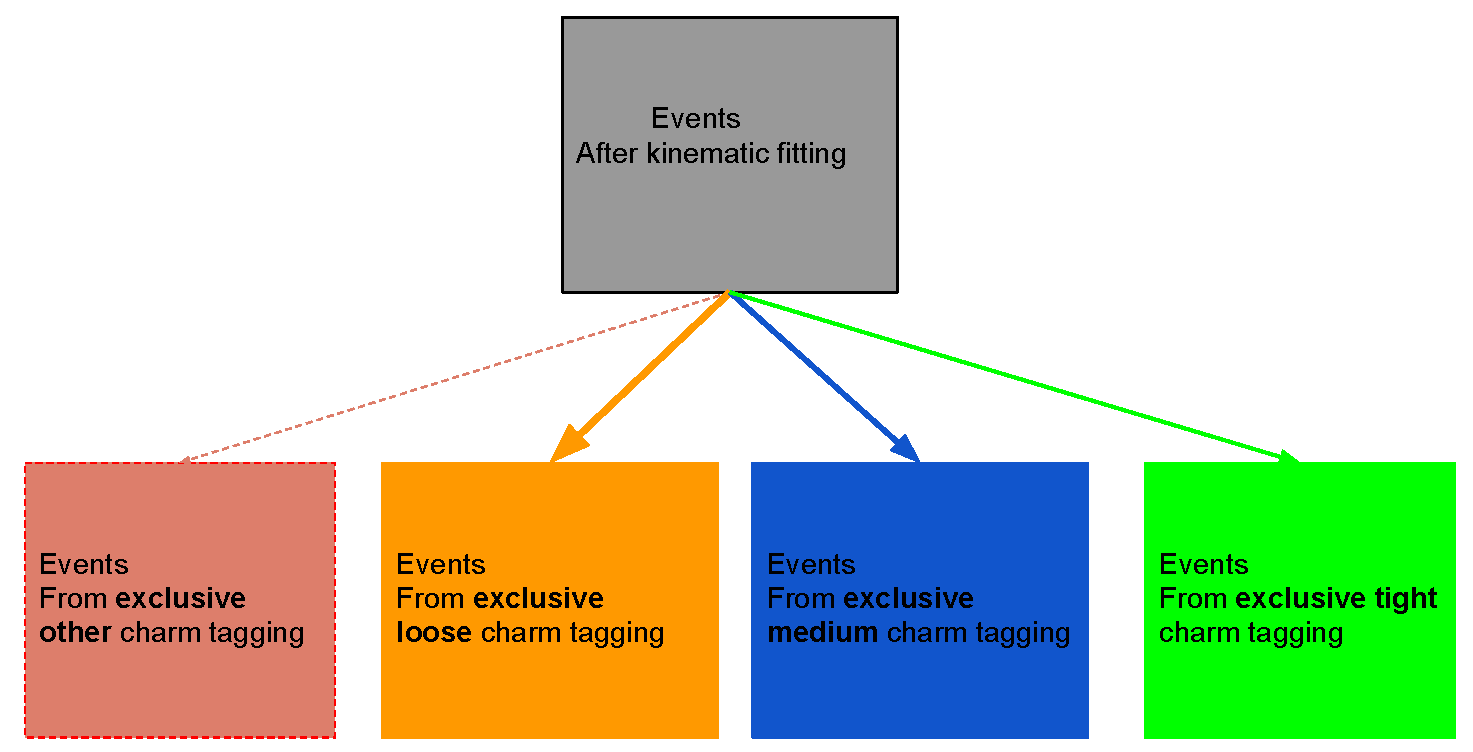
\includegraphics[width=1.00\textwidth]{Image/Limit/cTagCat.pdf}
\caption{Exclusive event categories based on charm-tagging.}
\label{fig:cTagCat}
\end{center}
\end{figure}
The \mjj distribution from exclusive charm categories is shown in 
Figure~\ref{fig:mjj_cTagEx}. The corresponding event yields are shown in 
Table~\ref{tab:eventYieldCTagEx}. The signal to background ratio (Sig/Bkg) is 
shown in Figures~\ref{fig:ratioSB_1},~\ref{fig:ratioSB_2} for different masses 
of charged Higgs for both channels. From these figures, one can see that the 
signal to background ratio is different in different categories. The 
corresponding systematics and statistical uncertainties from different sources 
are shown in Table~\ref{tab:sysCTagEx}. The data cards from these 3 categories 
are combined to compute limits as described in Sec.~\ref{ss:limit_cTagEx}. 

\begin{figure}
\centering  
\subfigure[]{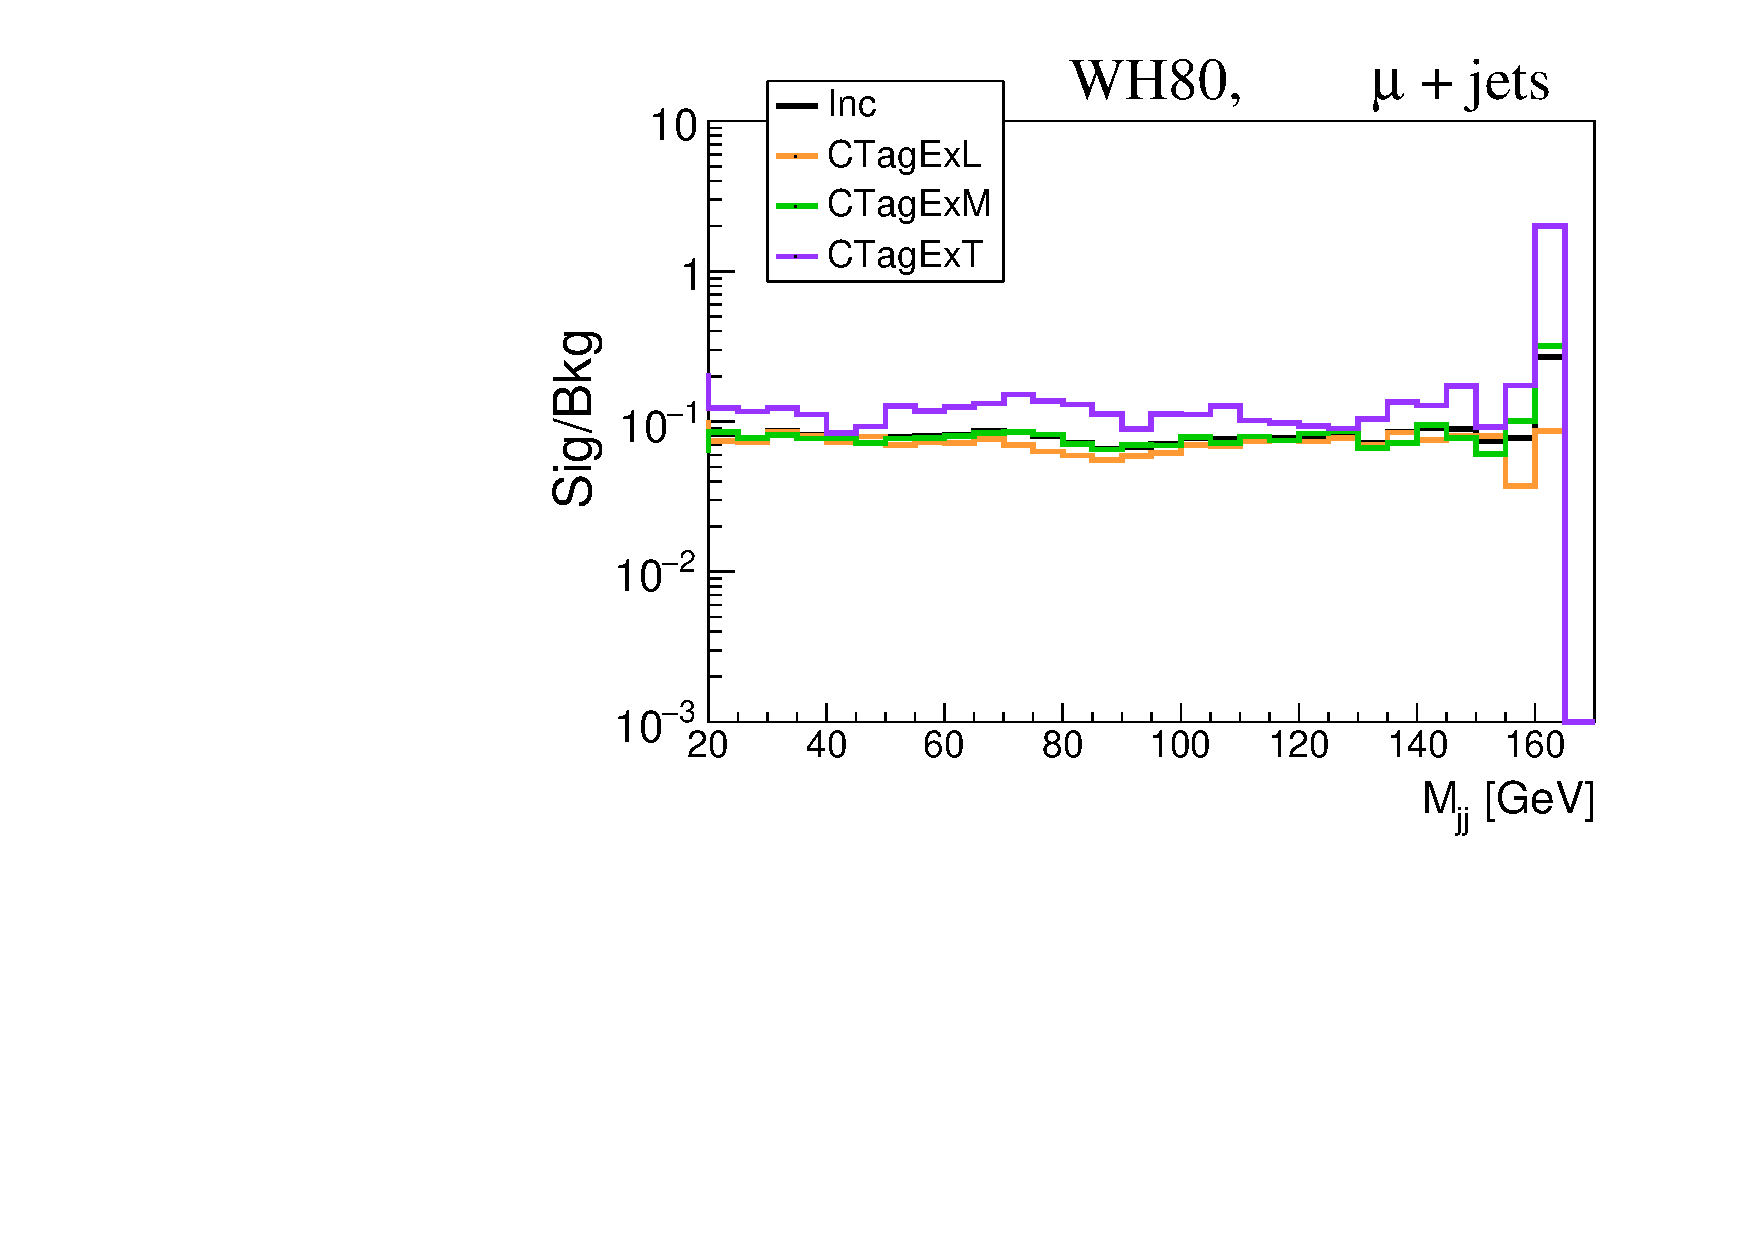
\includegraphics[width=0.45\linewidth]{Image/Muon/CTag/WH80_mu_ratioSB.pdf}}
\subfigure[]{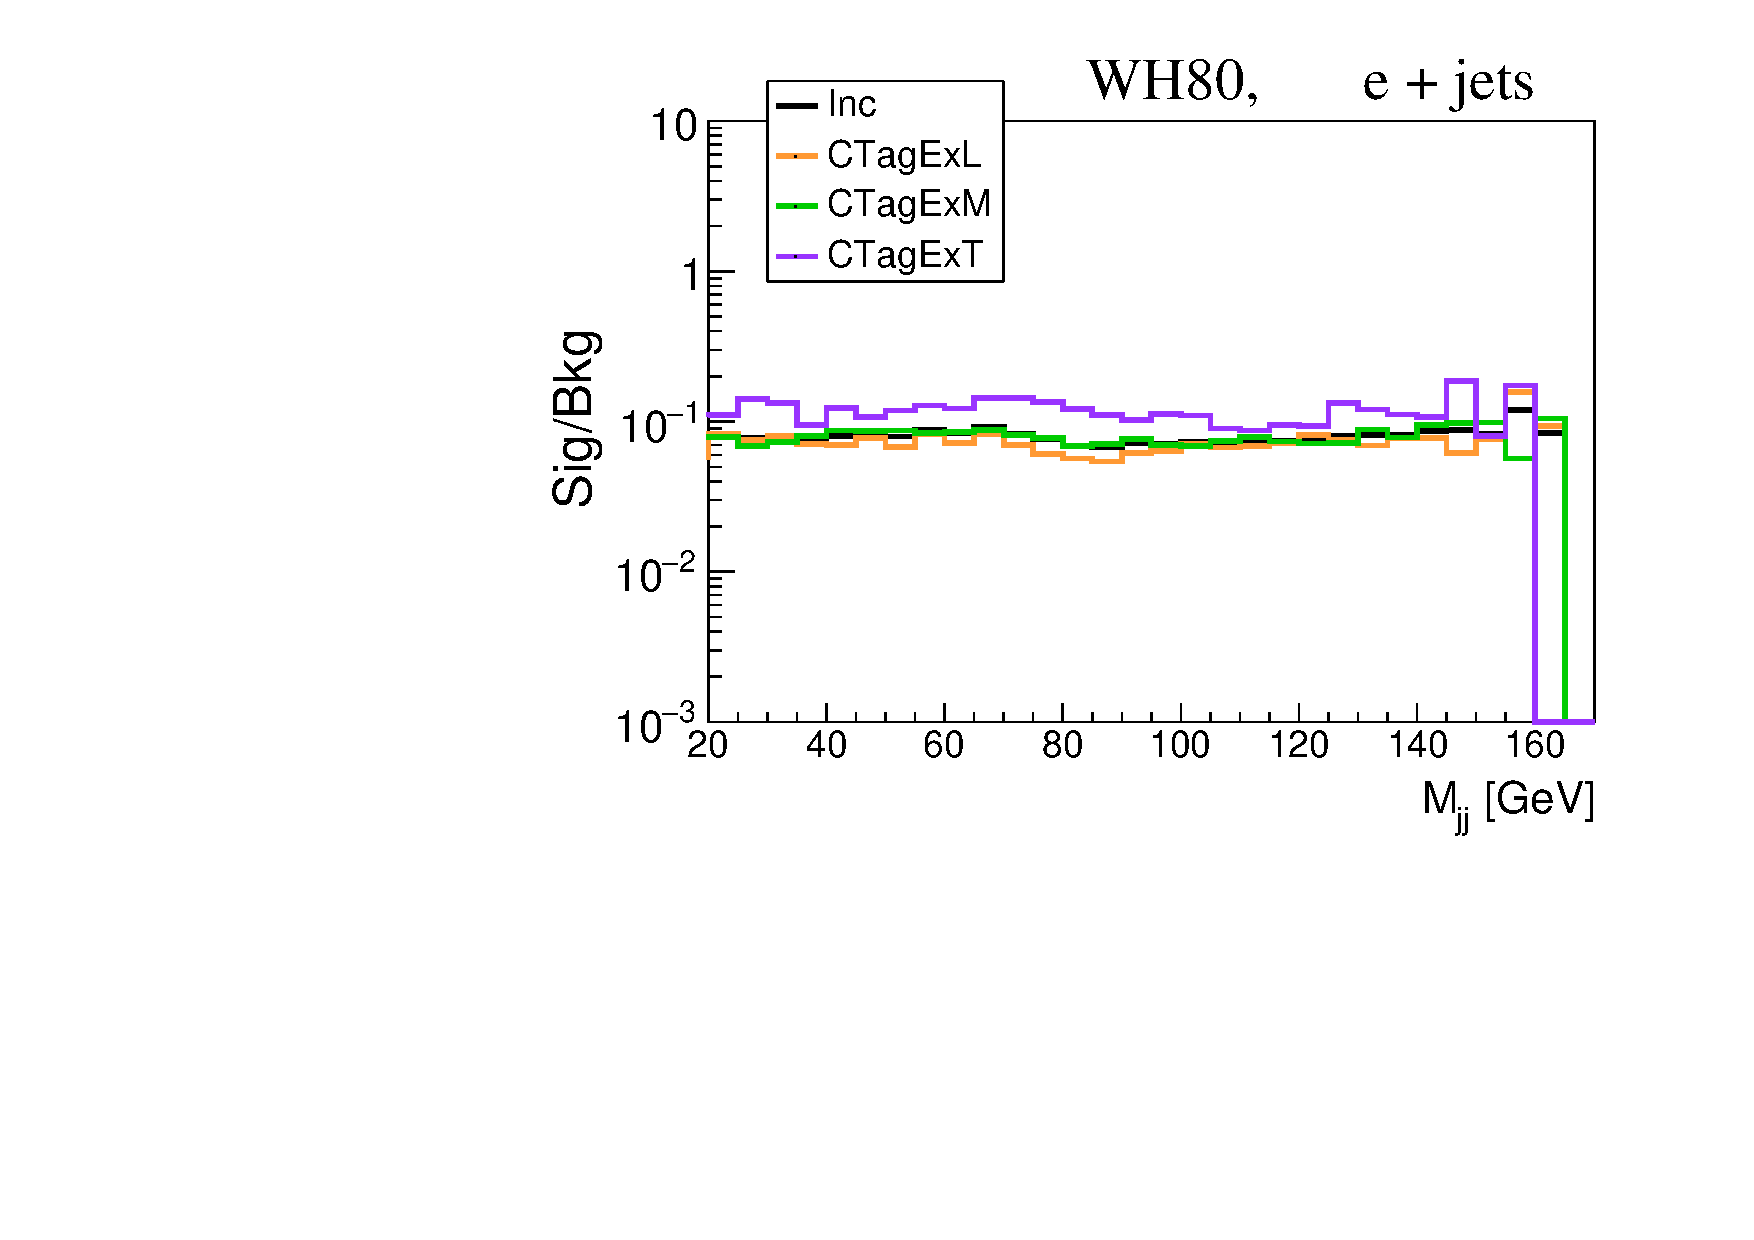
\includegraphics[width=0.45\linewidth]{Image/Electron/CTag/WH80_ele_ratioSB.pdf}}
\vfil
\subfigure[]{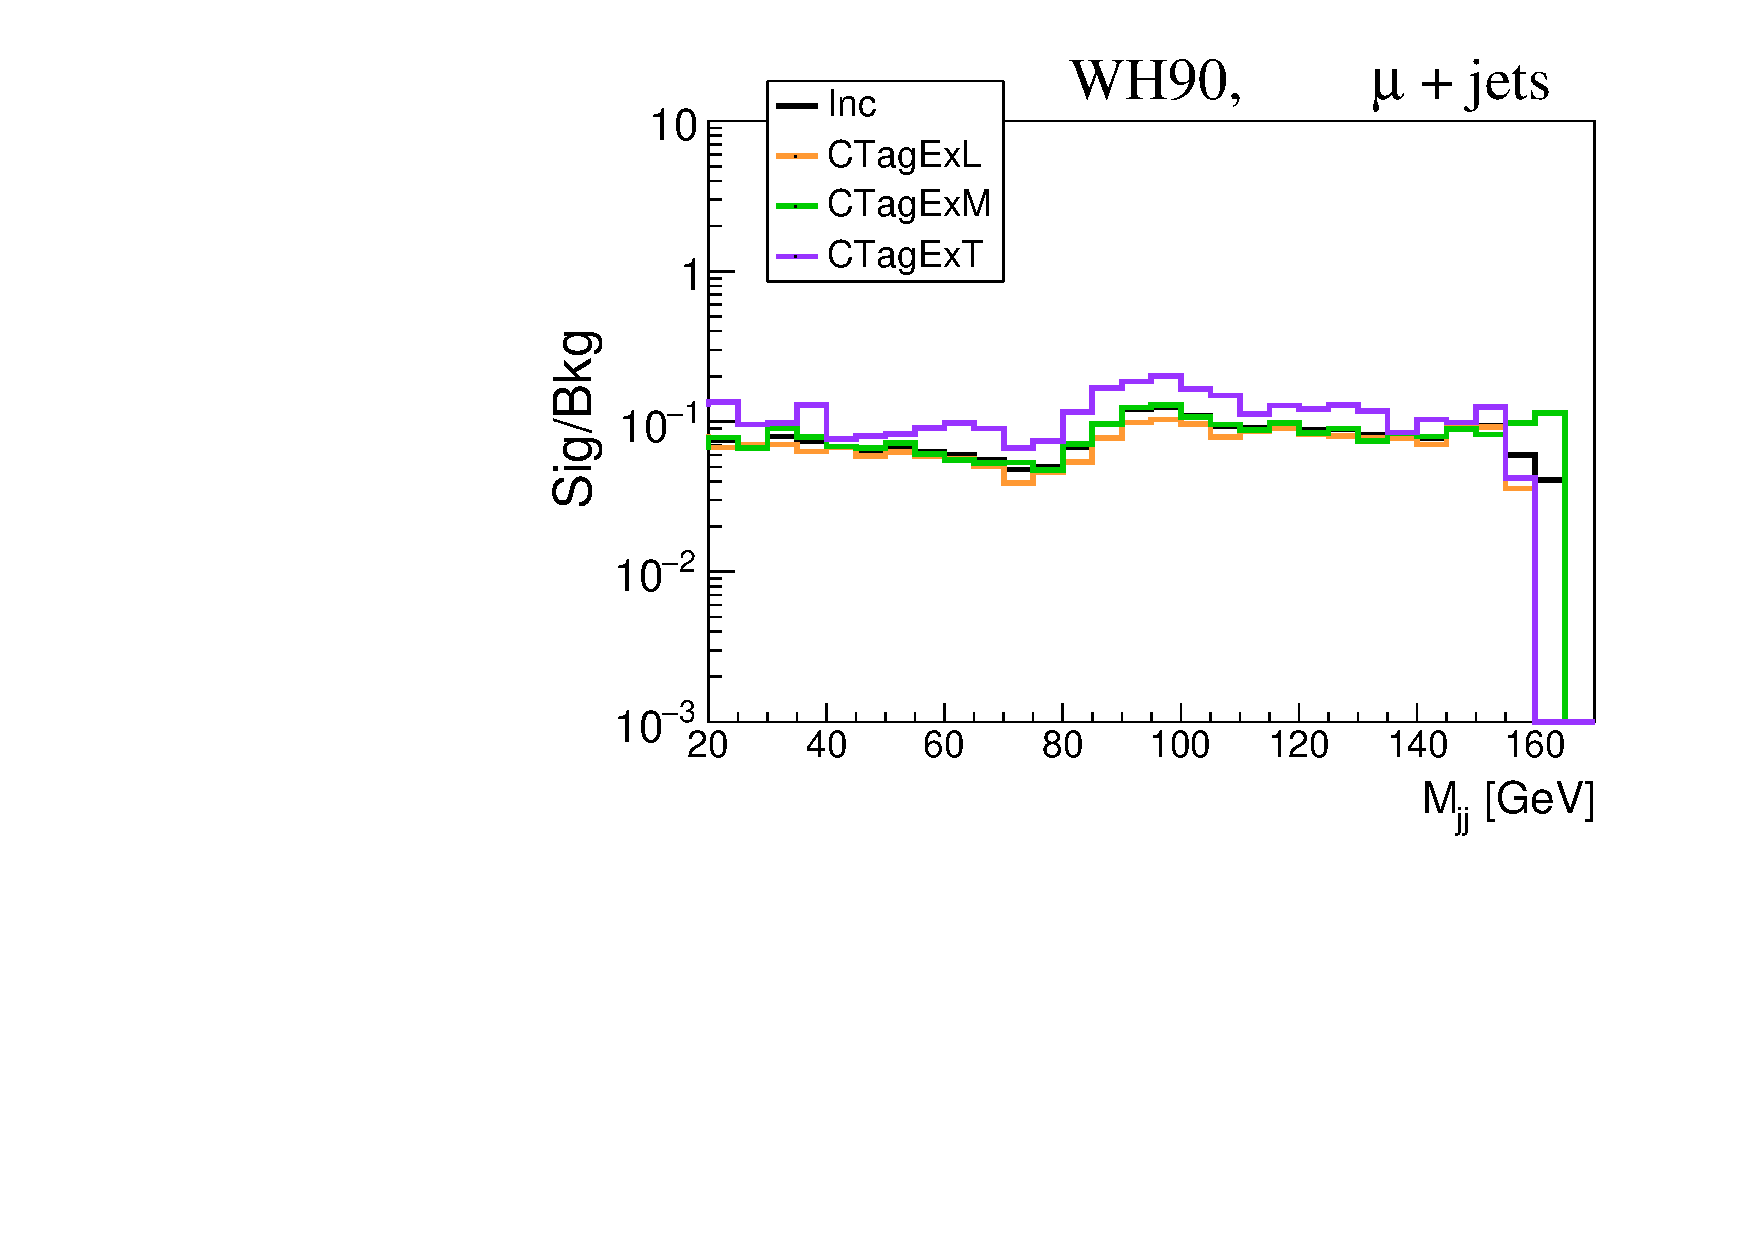
\includegraphics[width=0.45\linewidth]{Image/Muon/CTag/WH90_mu_ratioSB.pdf}}
\subfigure[]{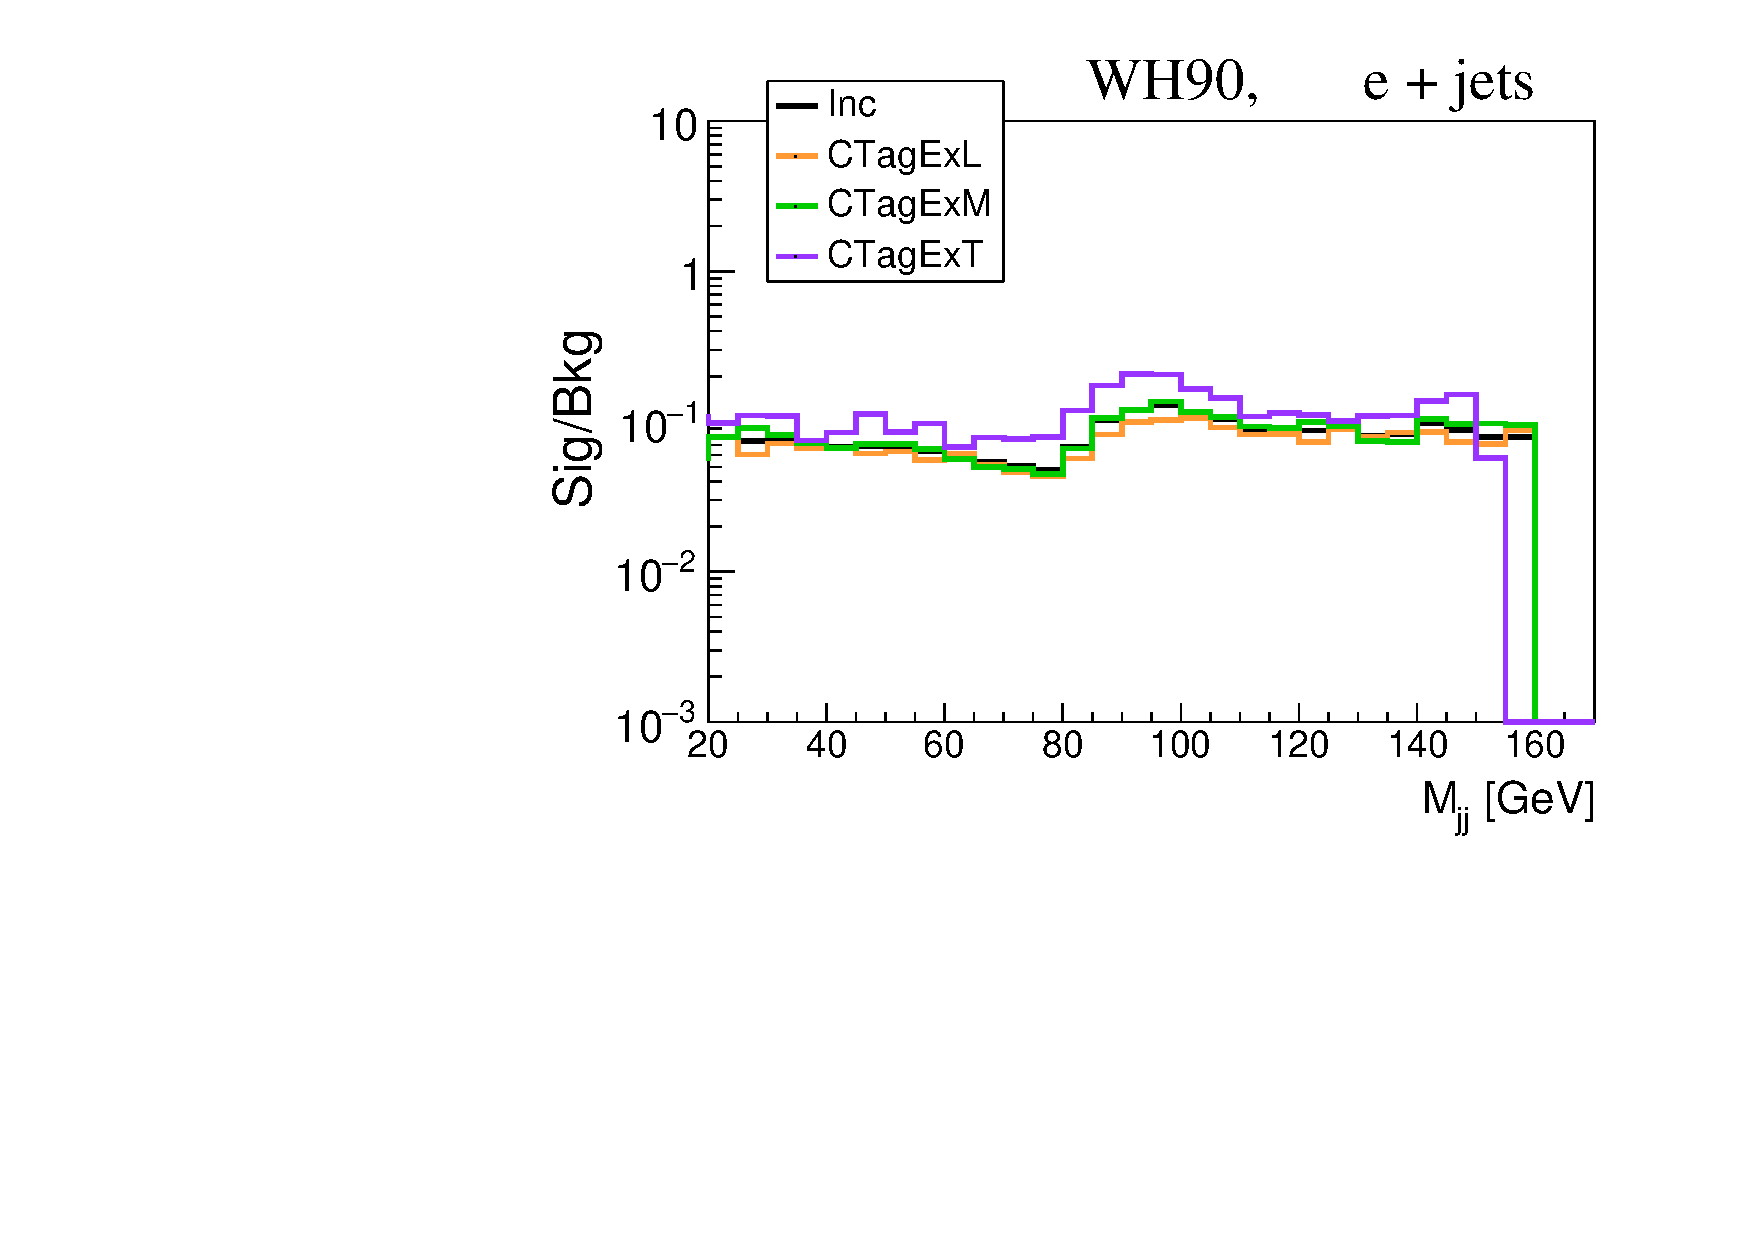
\includegraphics[width=0.45\linewidth]{Image/Electron/CTag/WH90_ele_ratioSB.pdf}}
\vfil
\subfigure[]{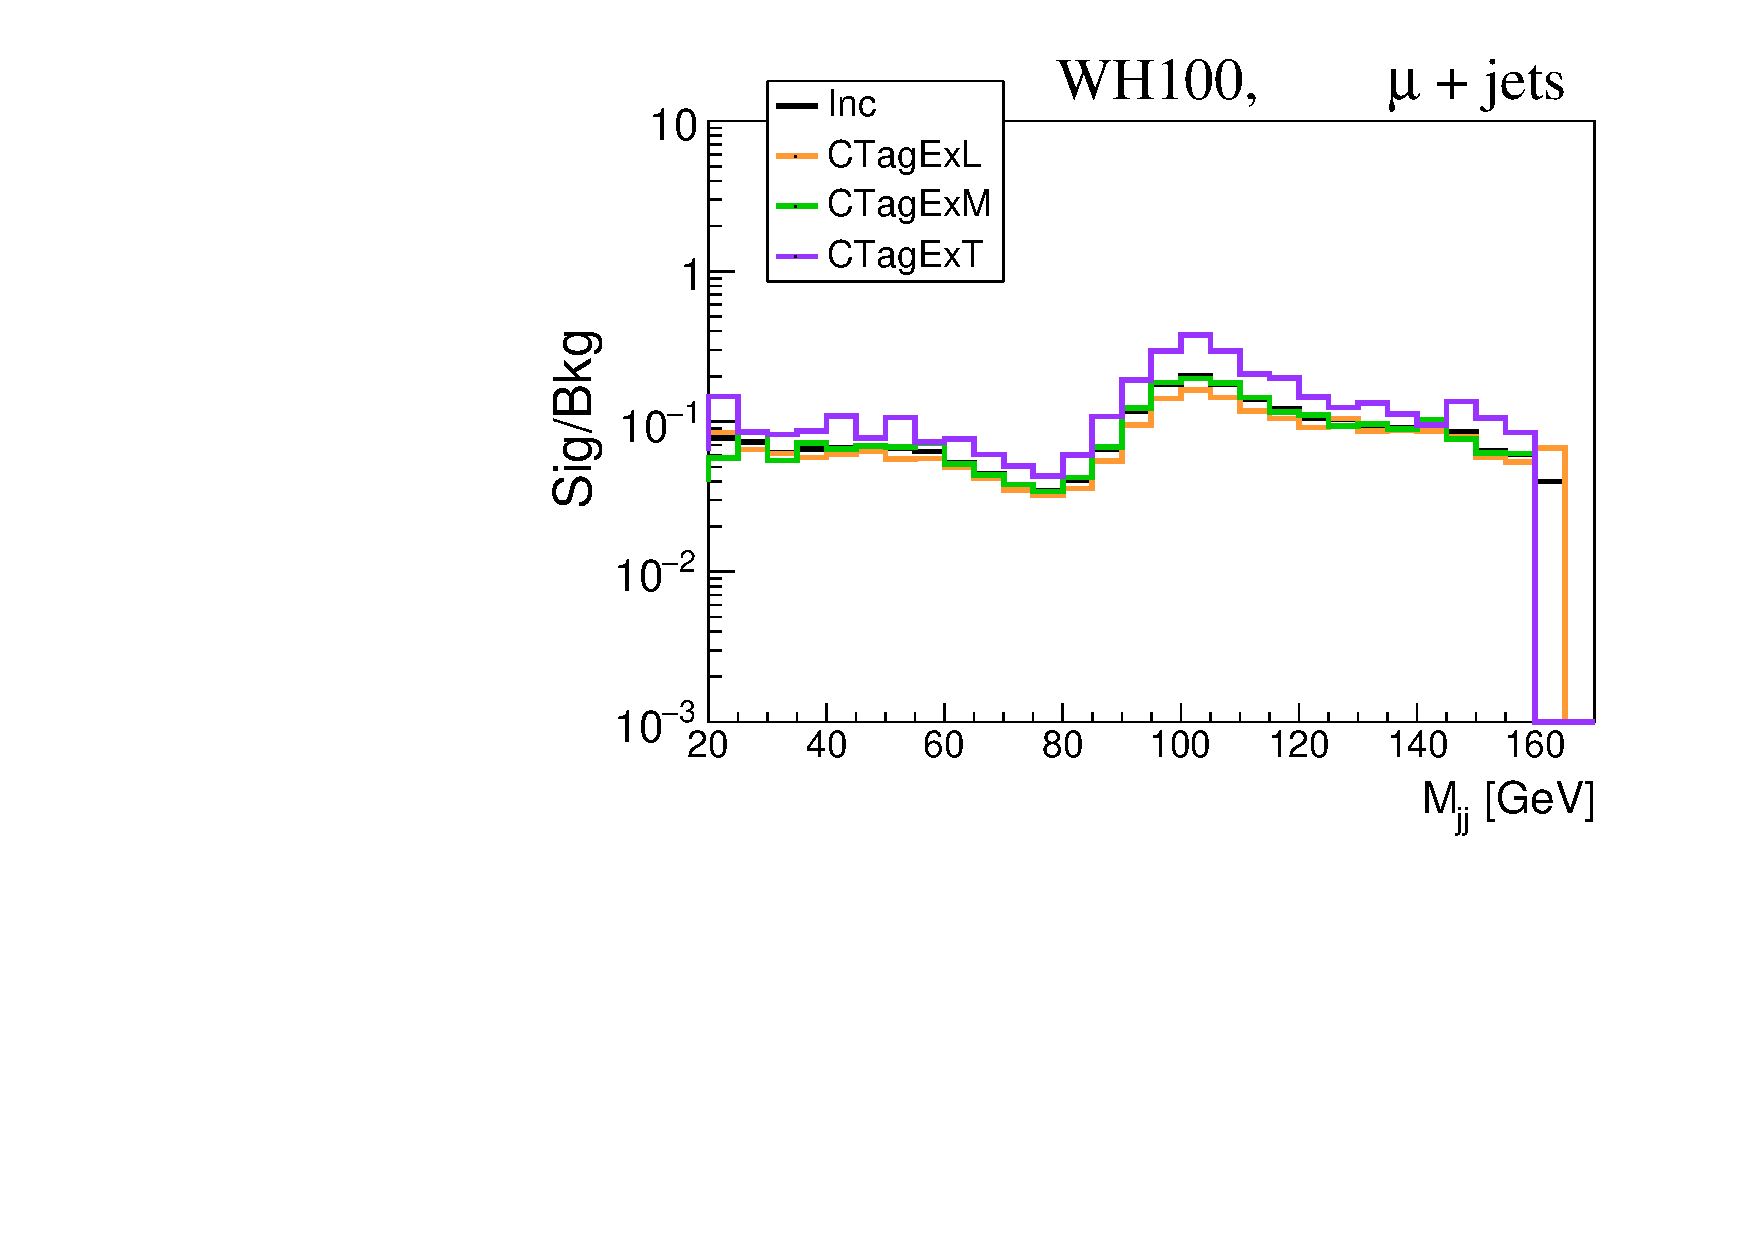
\includegraphics[width=0.45\linewidth]{Image/Muon/CTag/WH100_mu_ratioSB.pdf}}
\subfigure[]{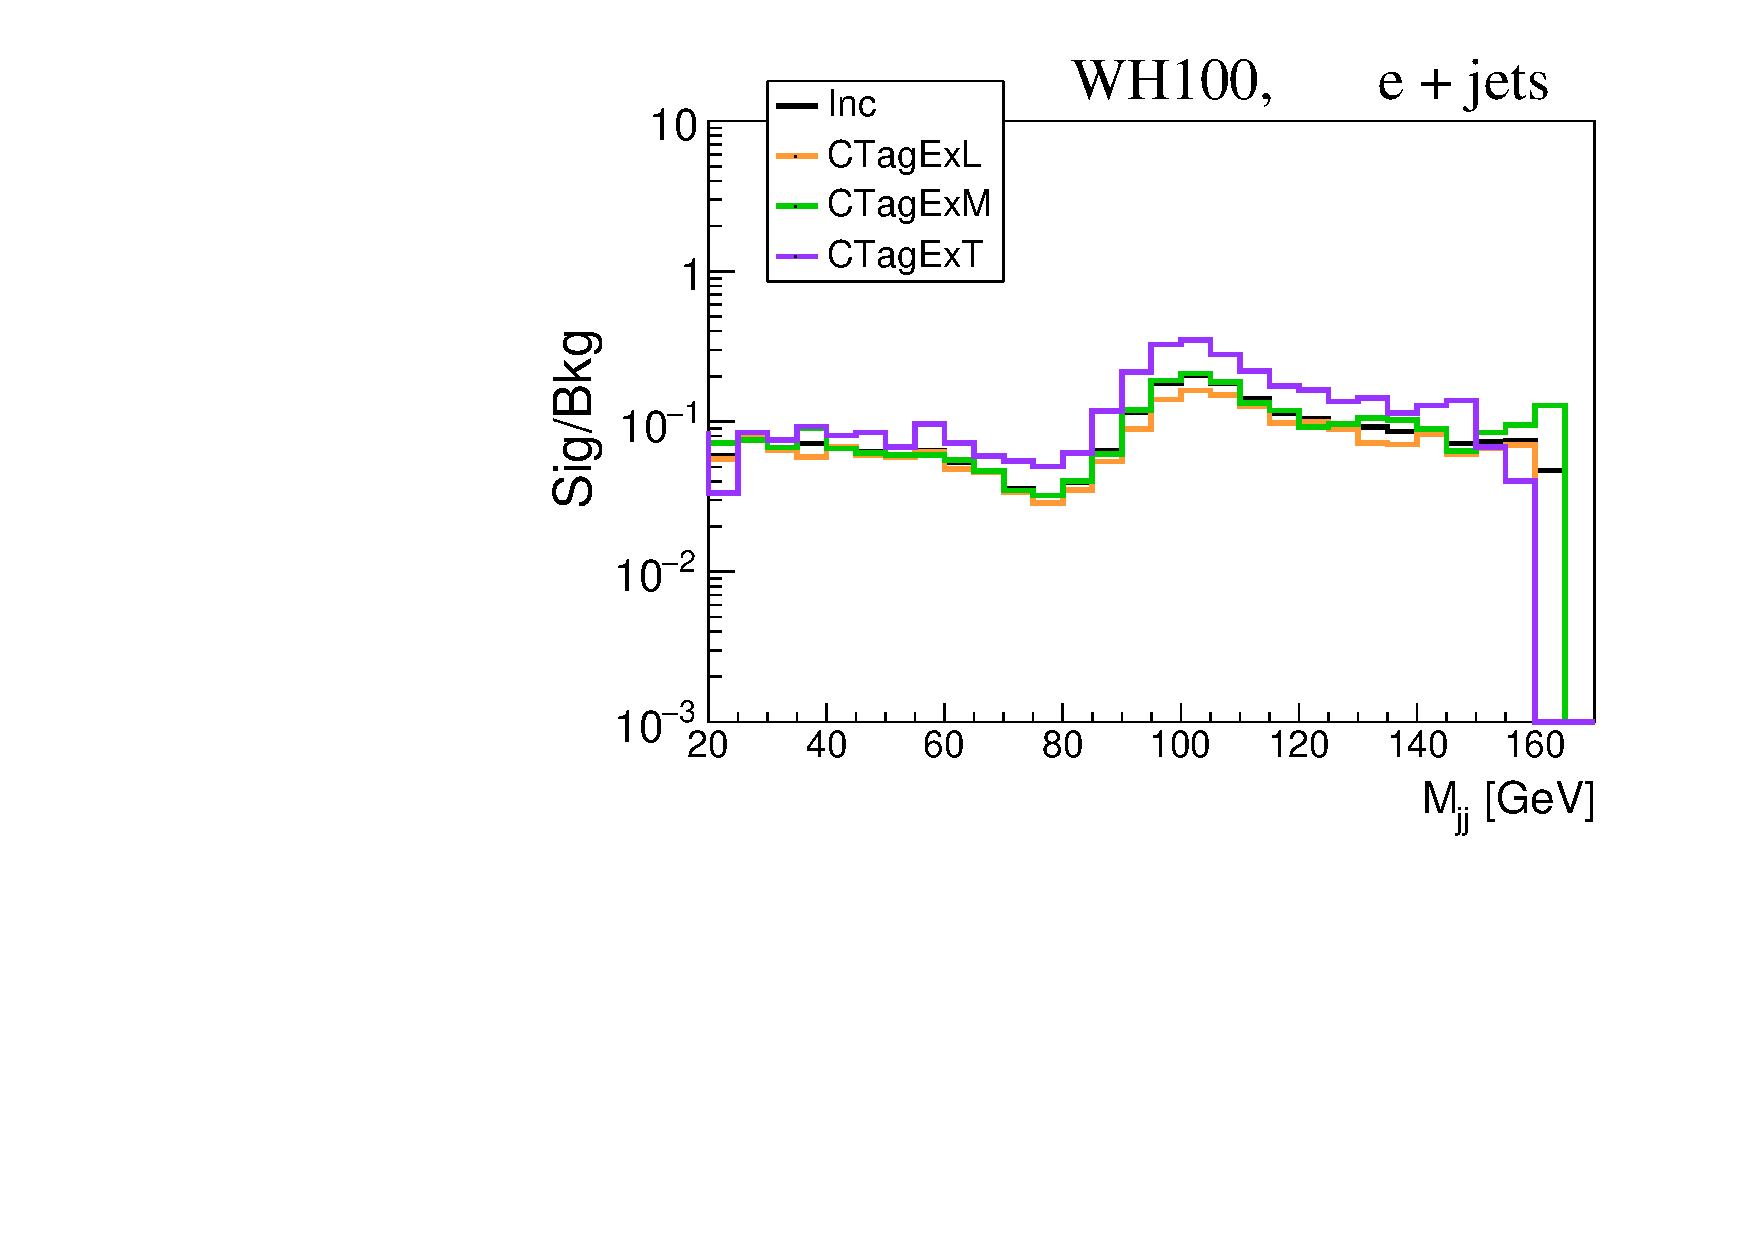
\includegraphics[width=0.45\linewidth]{Image/Electron/CTag/WH100_ele_ratioSB.pdf}}
\vfil
\subfigure[]{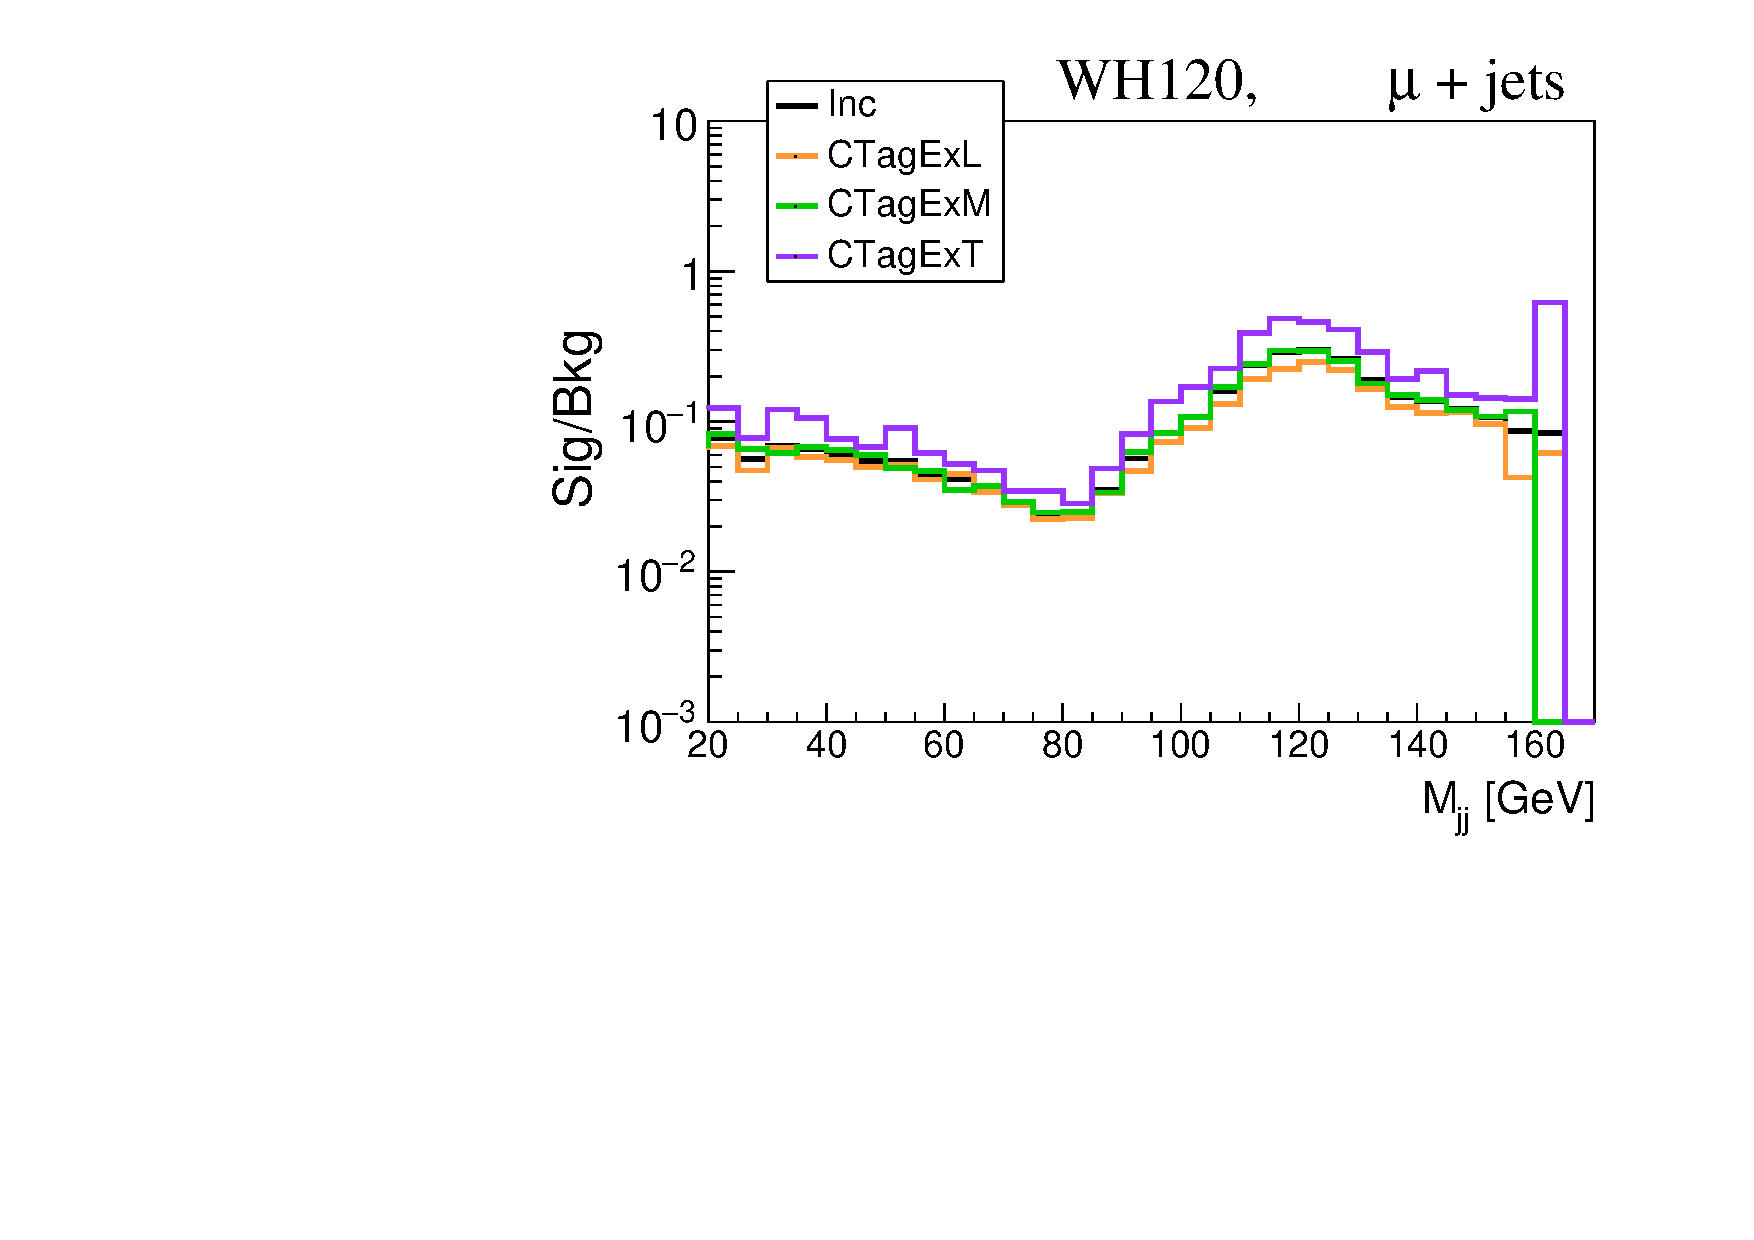
\includegraphics[width=0.45\linewidth]{Image/Muon/CTag/WH120_mu_ratioSB.pdf}}
\subfigure[]{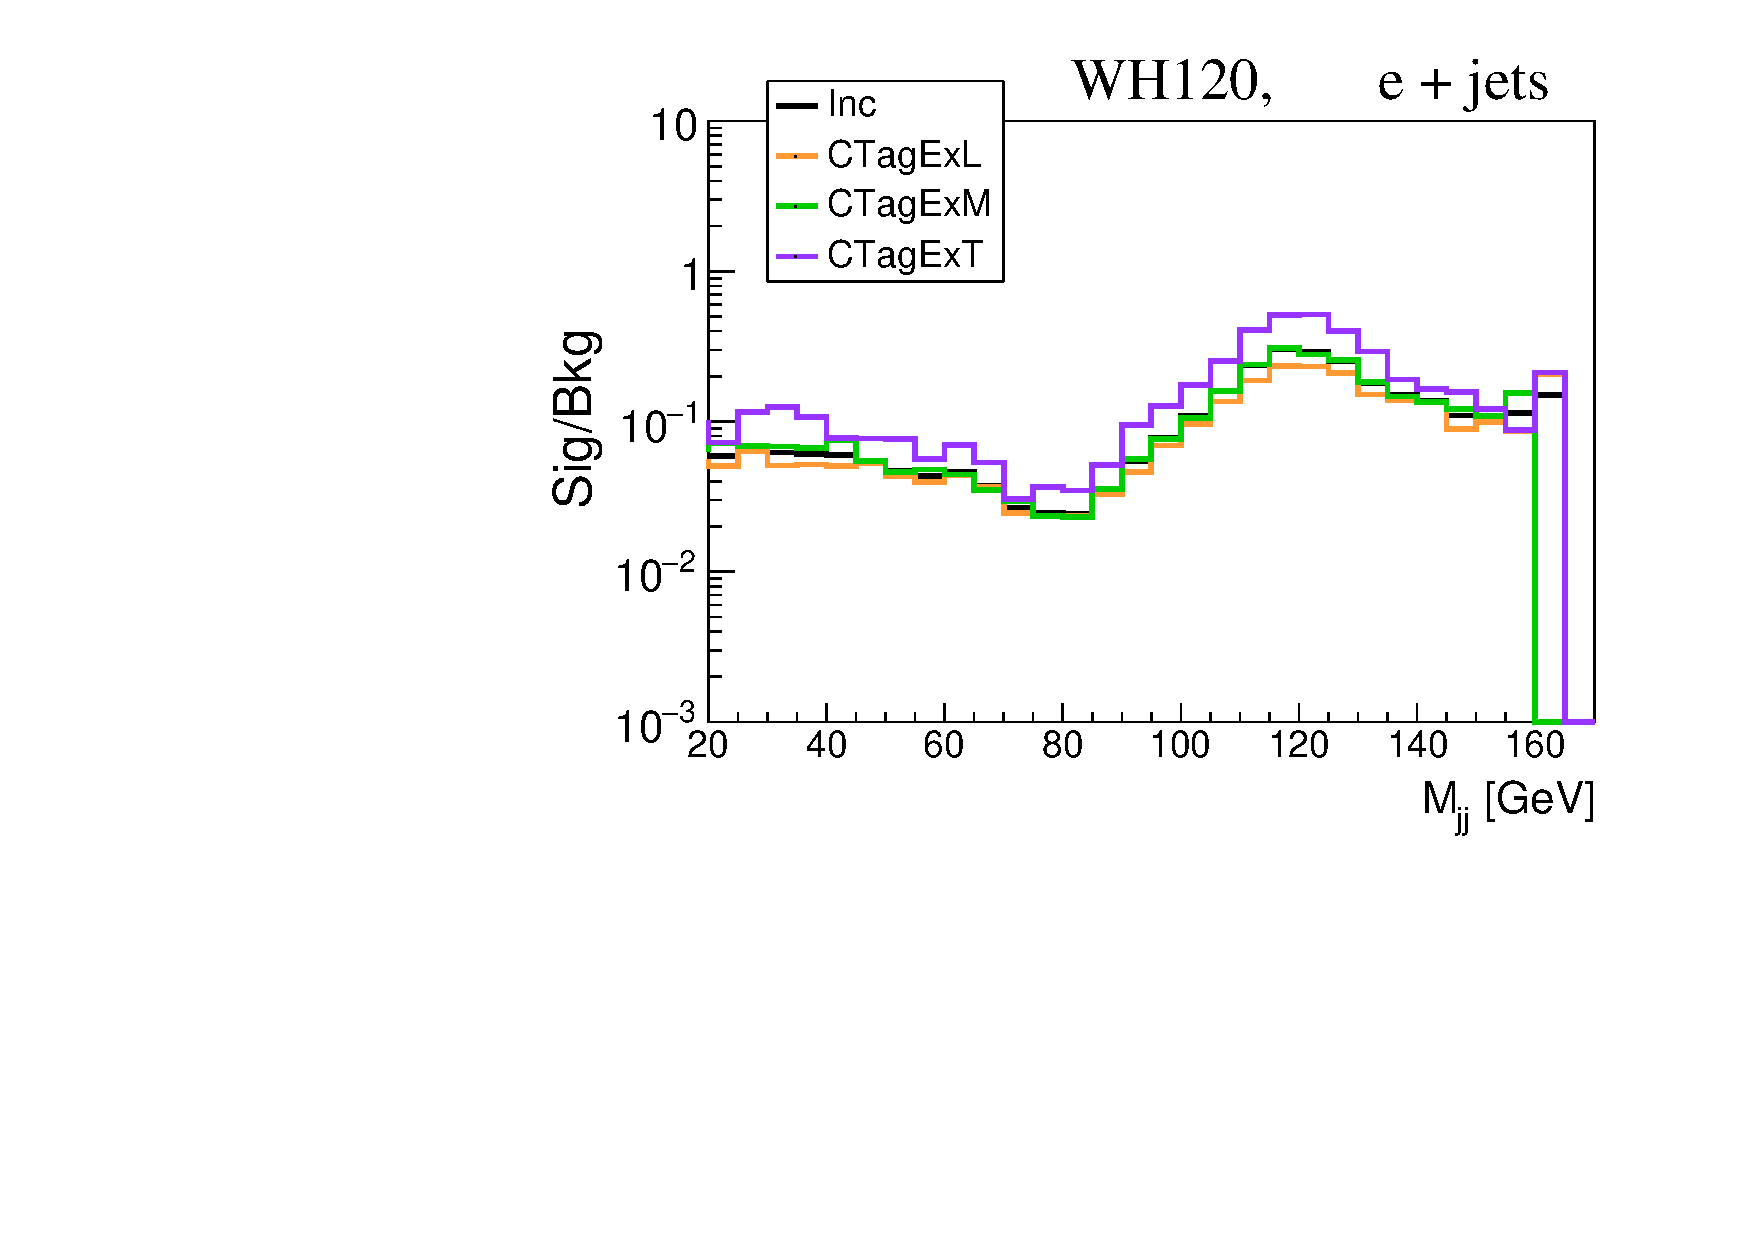
\includegraphics[width=0.45\linewidth]{Image/Electron/CTag/WH120_ele_ratioSB.pdf}}
\caption{Signal to background ratio for $m_{H^+}$ = 80, 90, 100, 120 GeV.}
\label{fig:ratioSB_1}
\end{figure}
\begin{figure}
\centering  
\subfigure[]{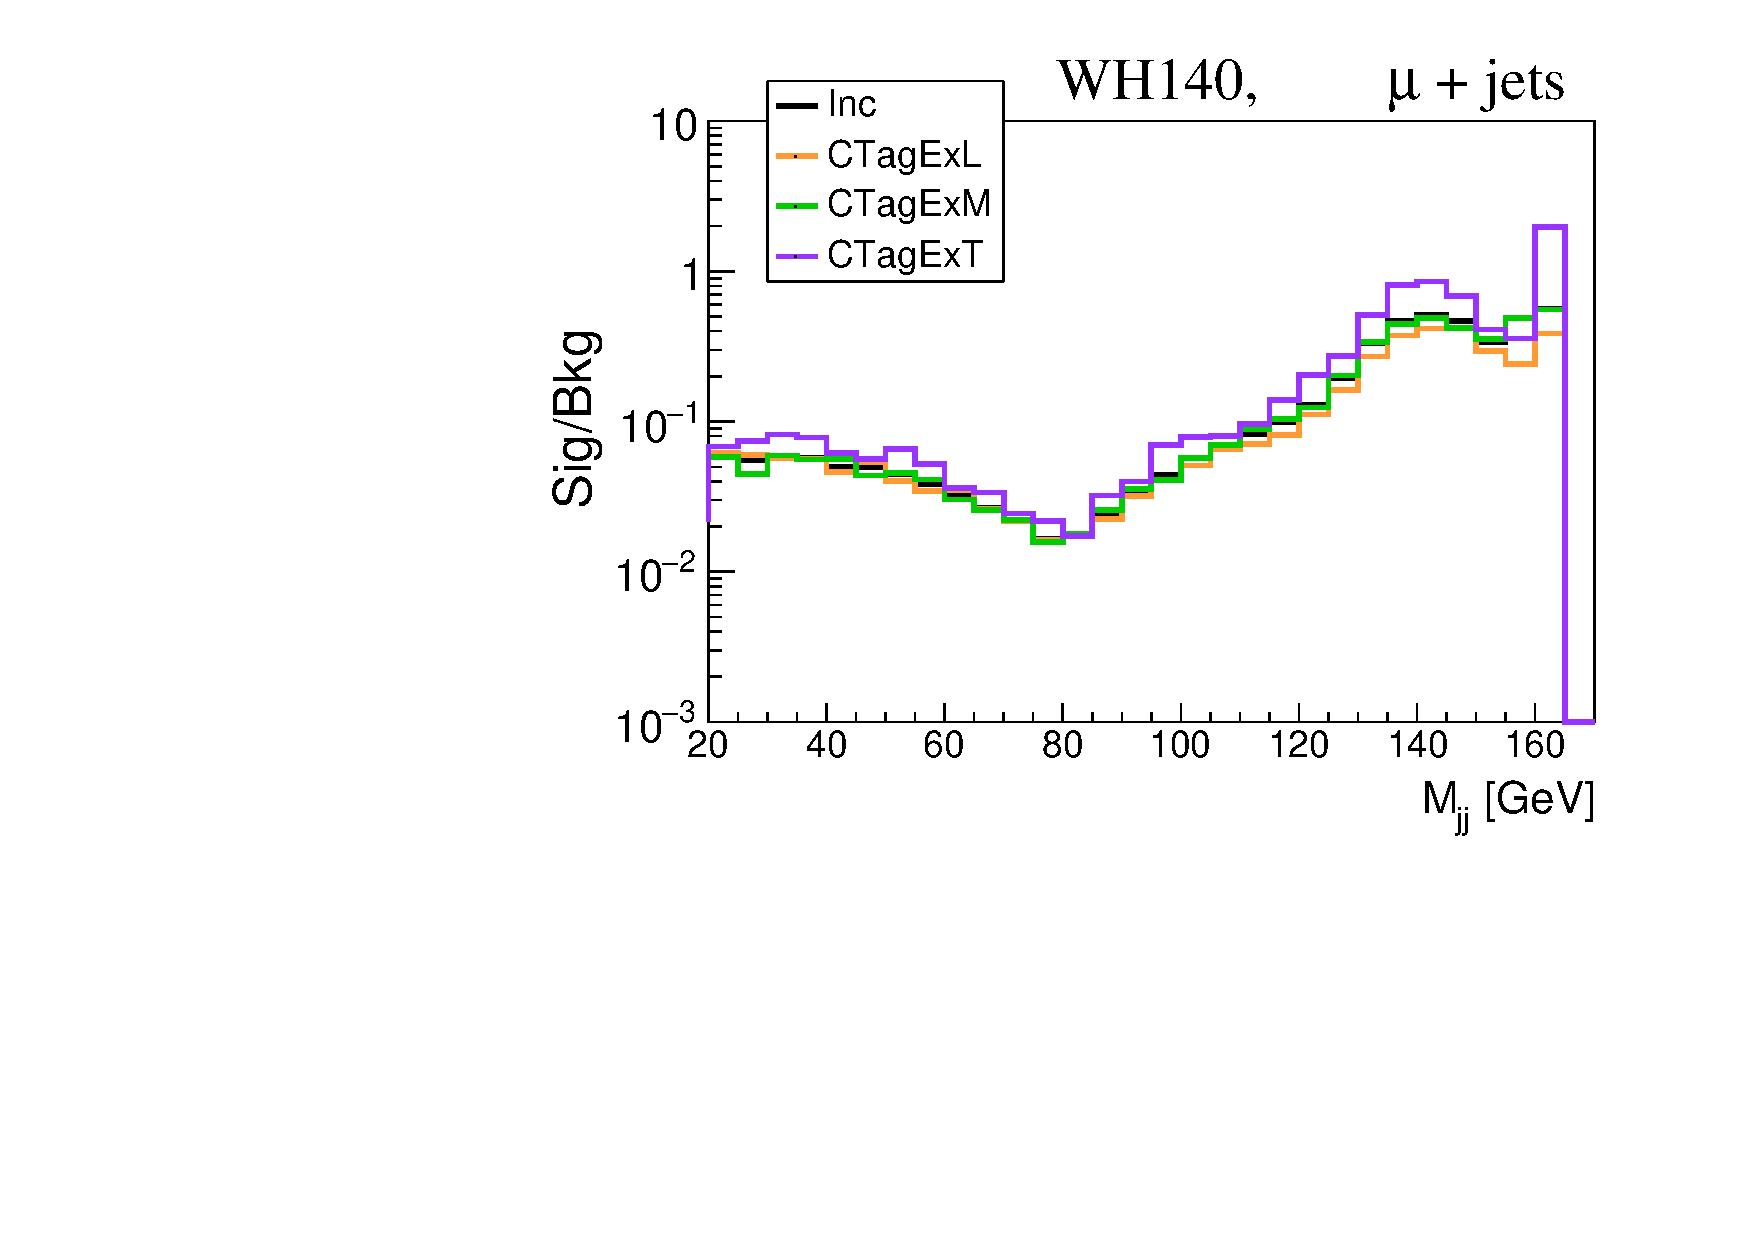
\includegraphics[width=0.45\linewidth]{Image/Muon/CTag/WH140_mu_ratioSB.pdf}}
\subfigure[]{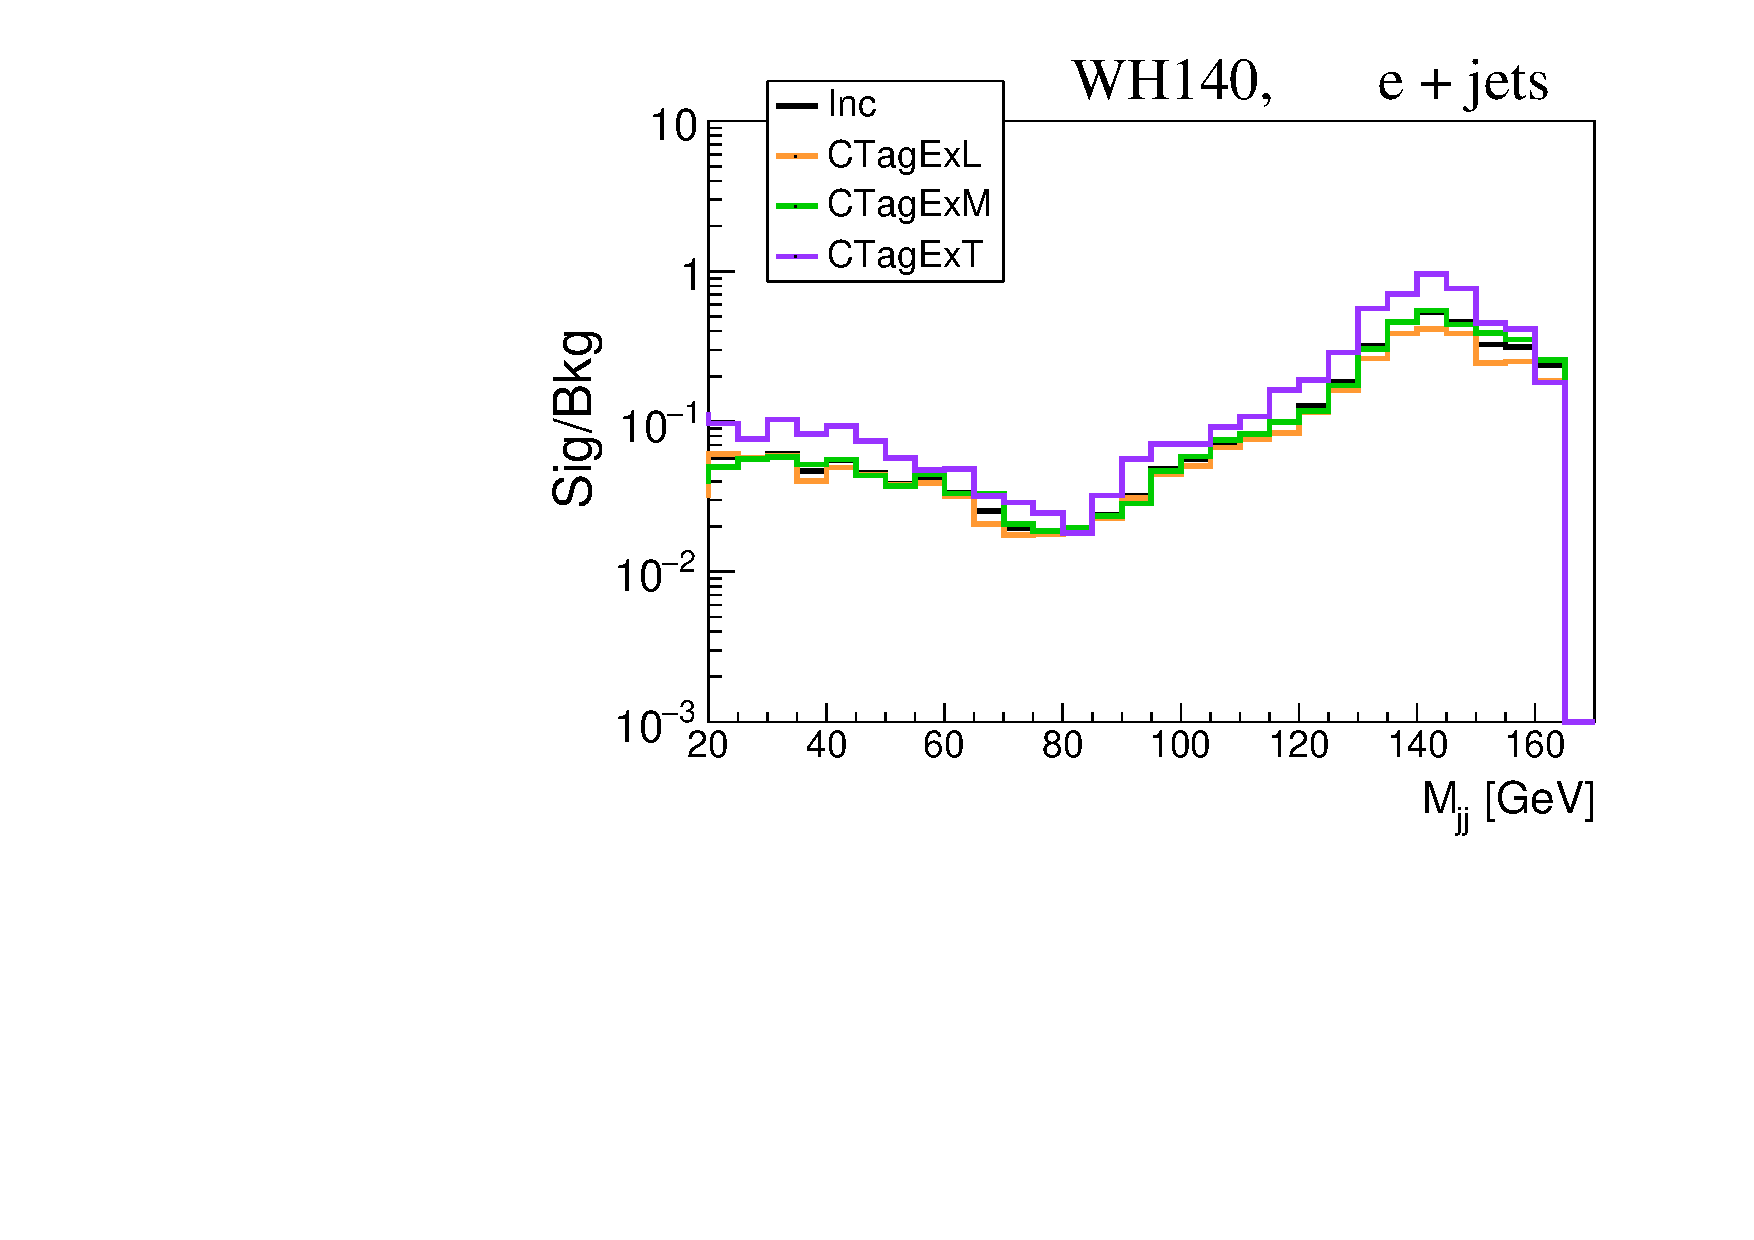
\includegraphics[width=0.45\linewidth]{Image/Electron/CTag/WH140_ele_ratioSB.pdf}}
\vfil
\subfigure[]{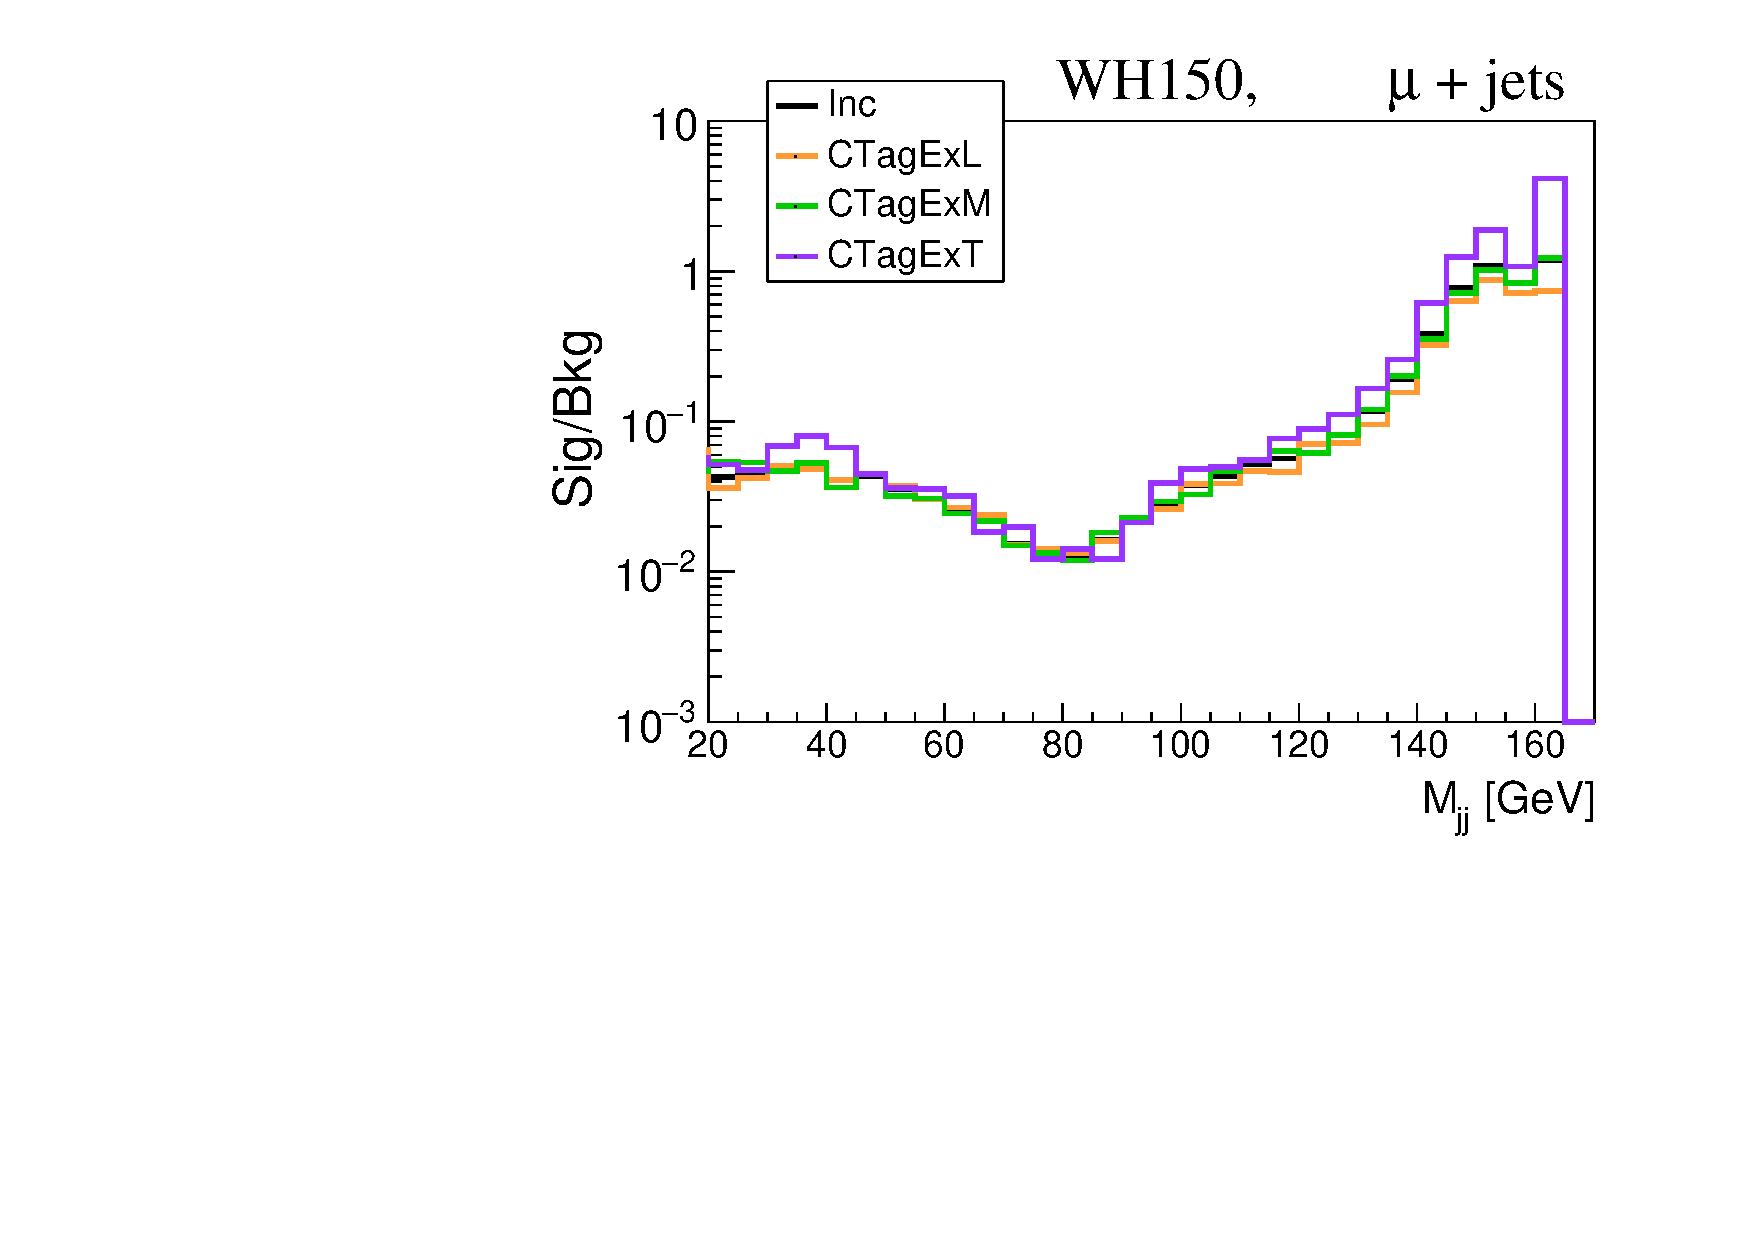
\includegraphics[width=0.45\linewidth]{Image/Muon/CTag/WH150_mu_ratioSB.pdf}}
\subfigure[]{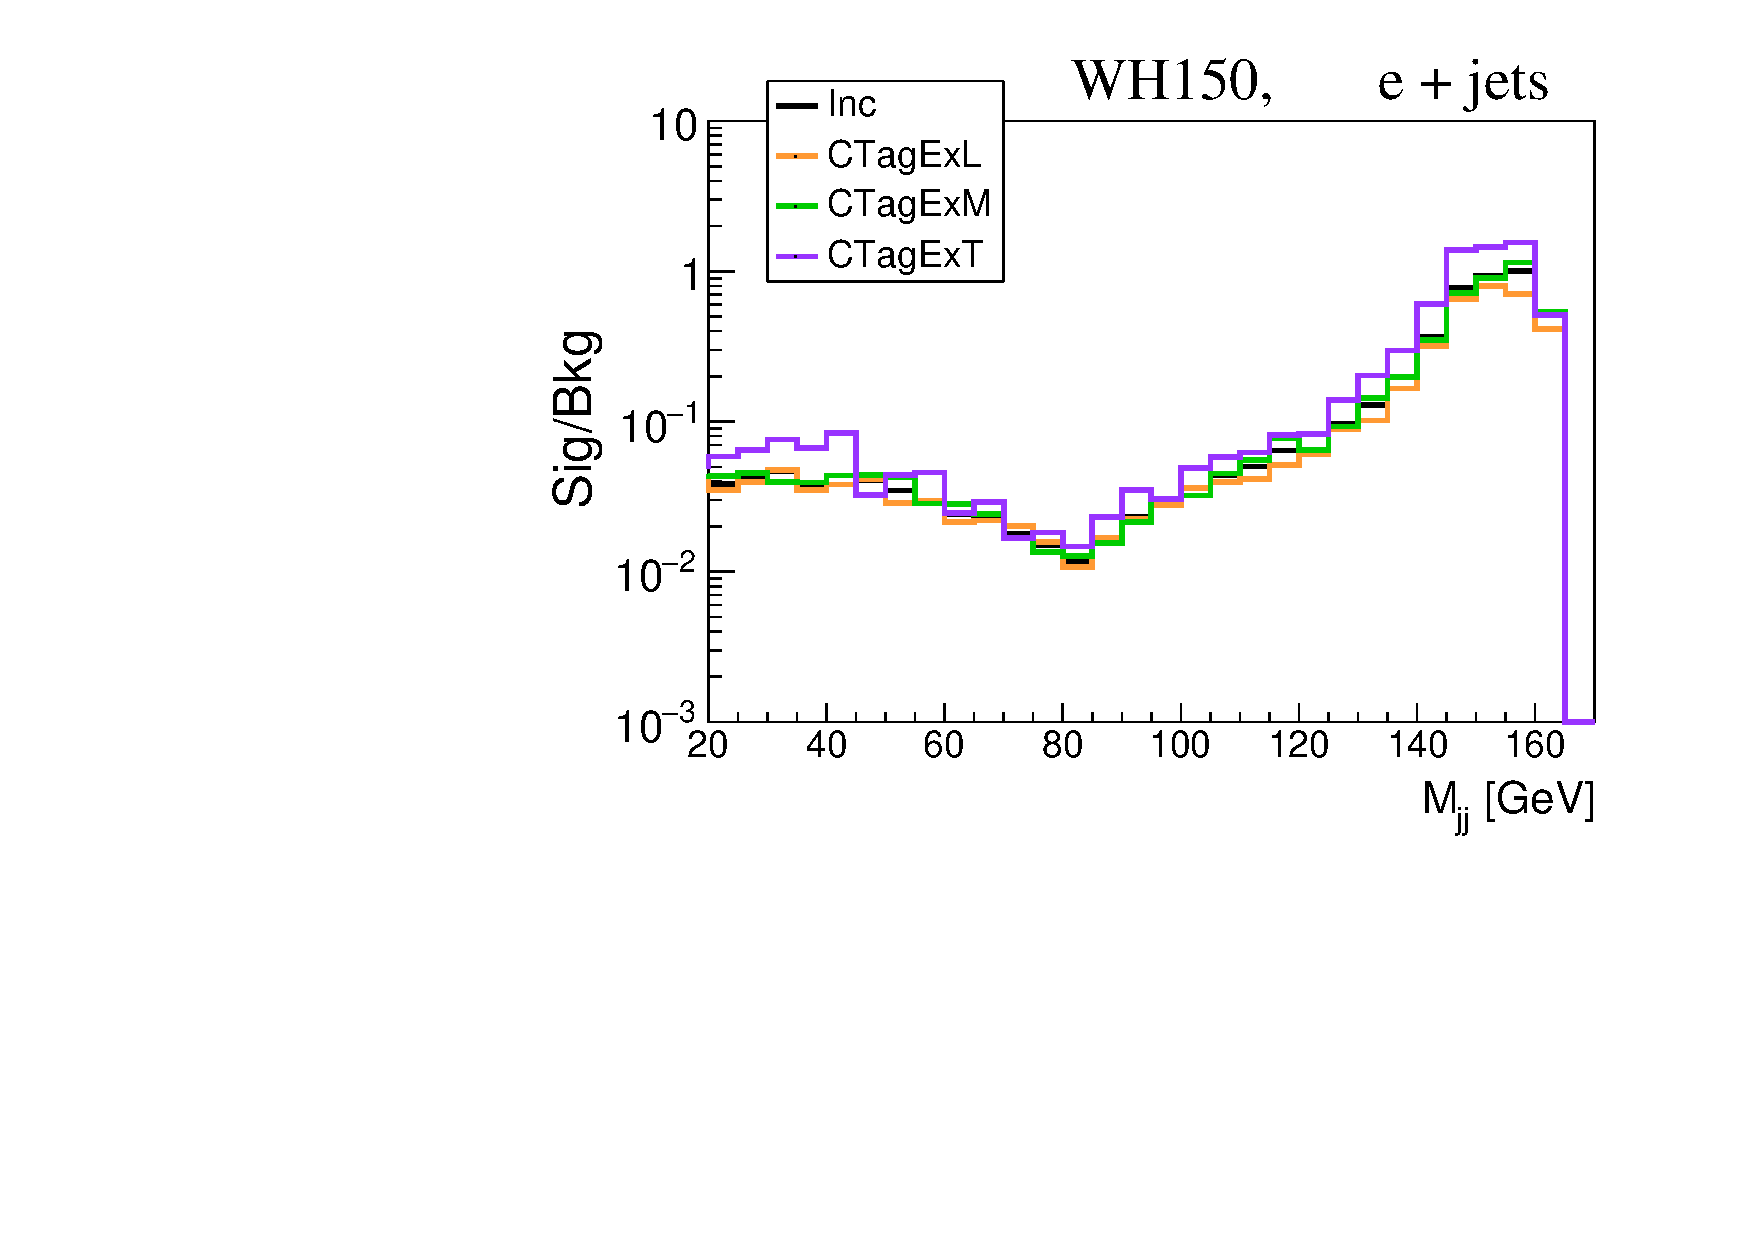
\includegraphics[width=0.45\linewidth]{Image/Electron/CTag/WH150_ele_ratioSB.pdf}}
\vfil
\subfigure[]{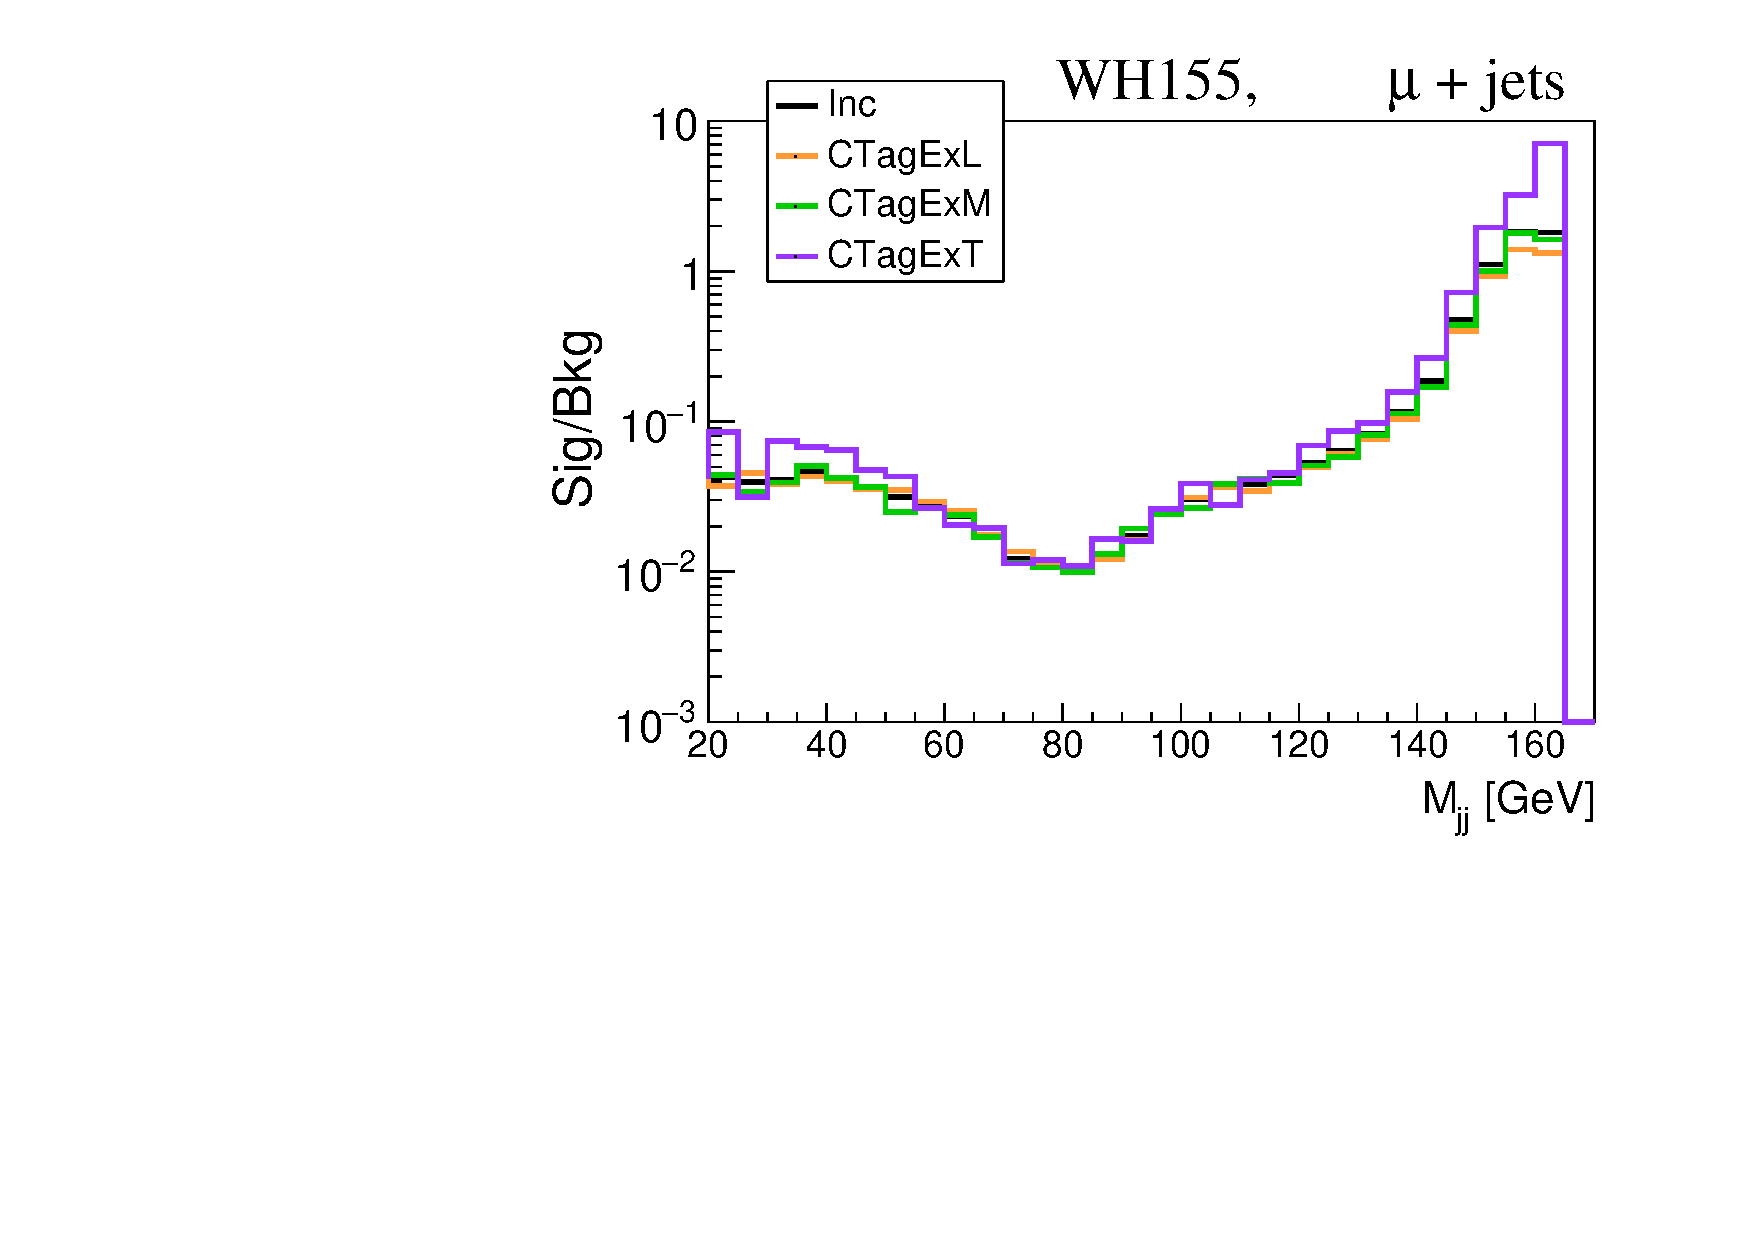
\includegraphics[width=0.45\linewidth]{Image/Muon/CTag/WH155_mu_ratioSB.pdf}}
\subfigure[]{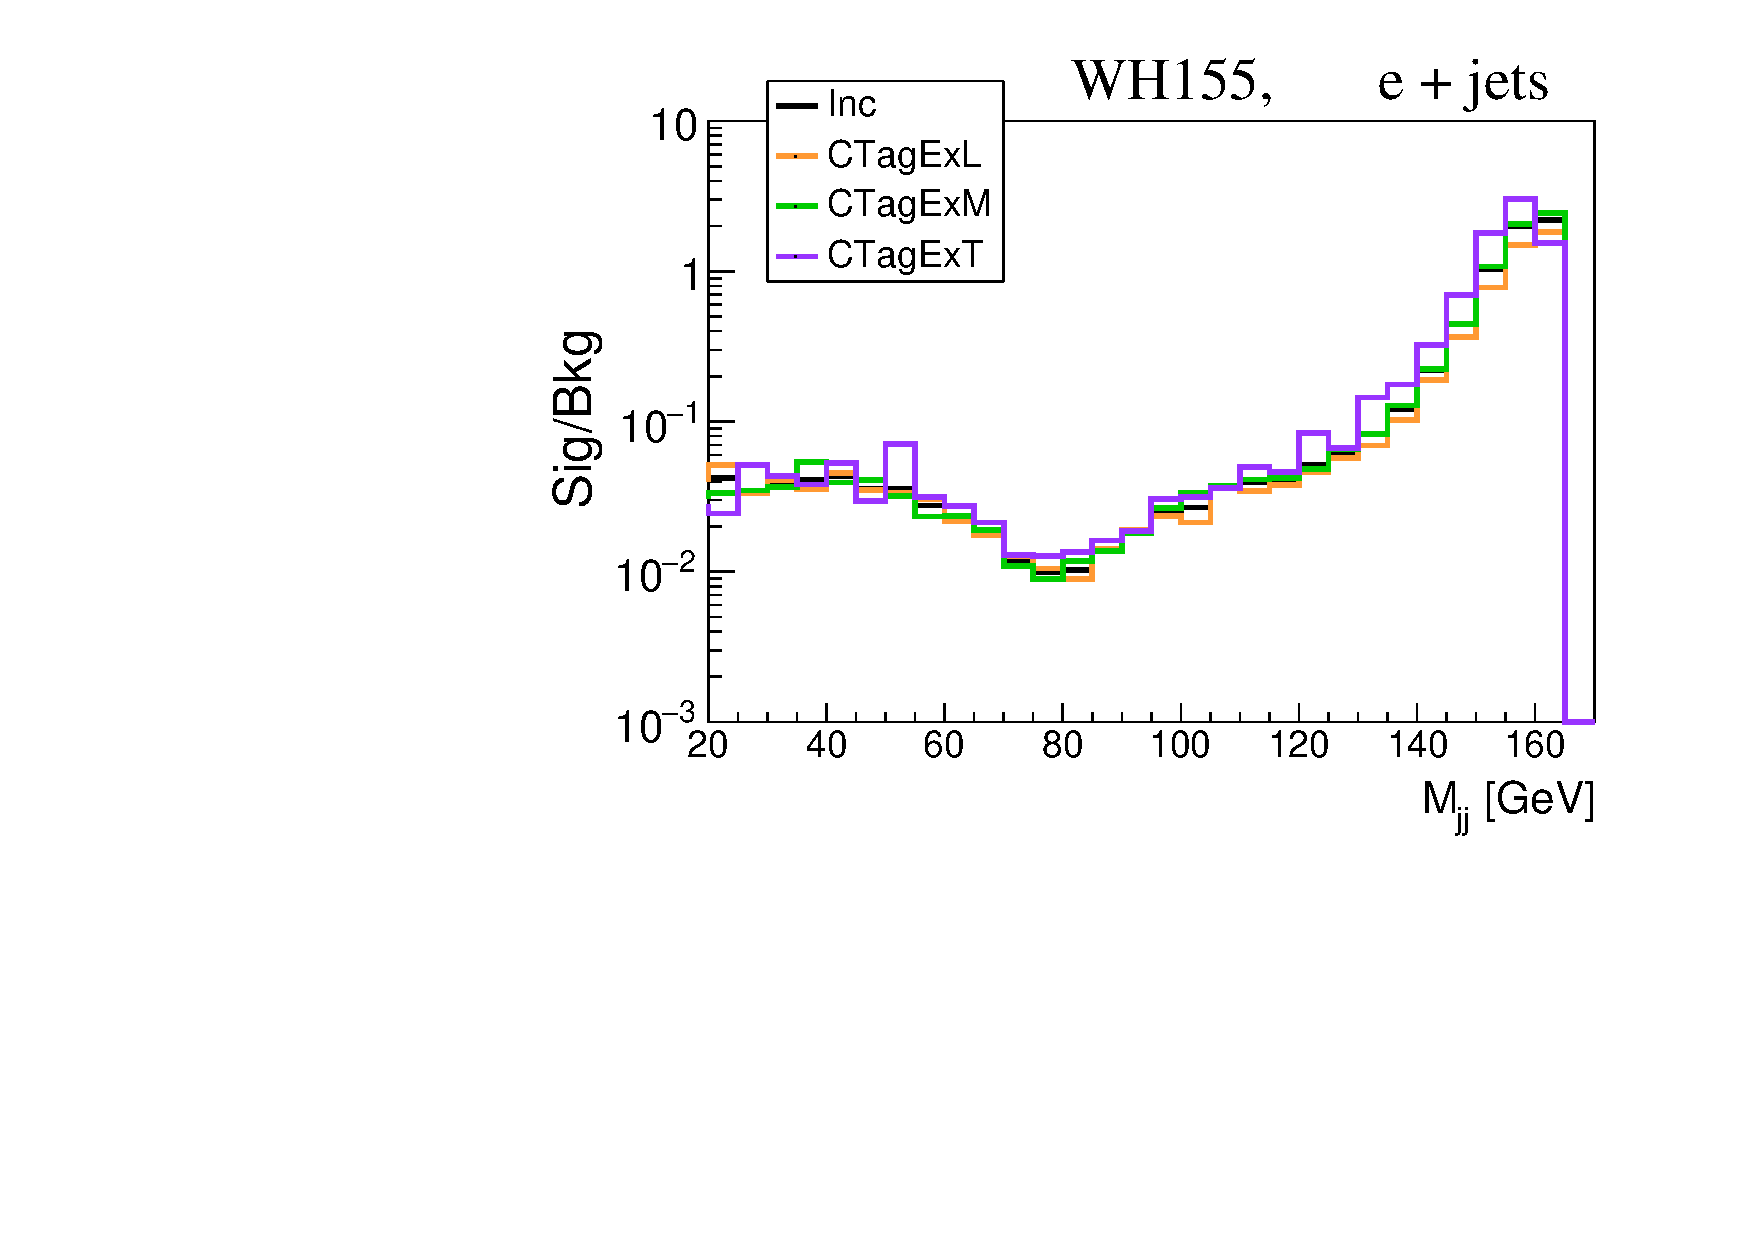
\includegraphics[width=0.45\linewidth]{Image/Electron/CTag/WH155_ele_ratioSB.pdf}}
\vfil
\subfigure[]{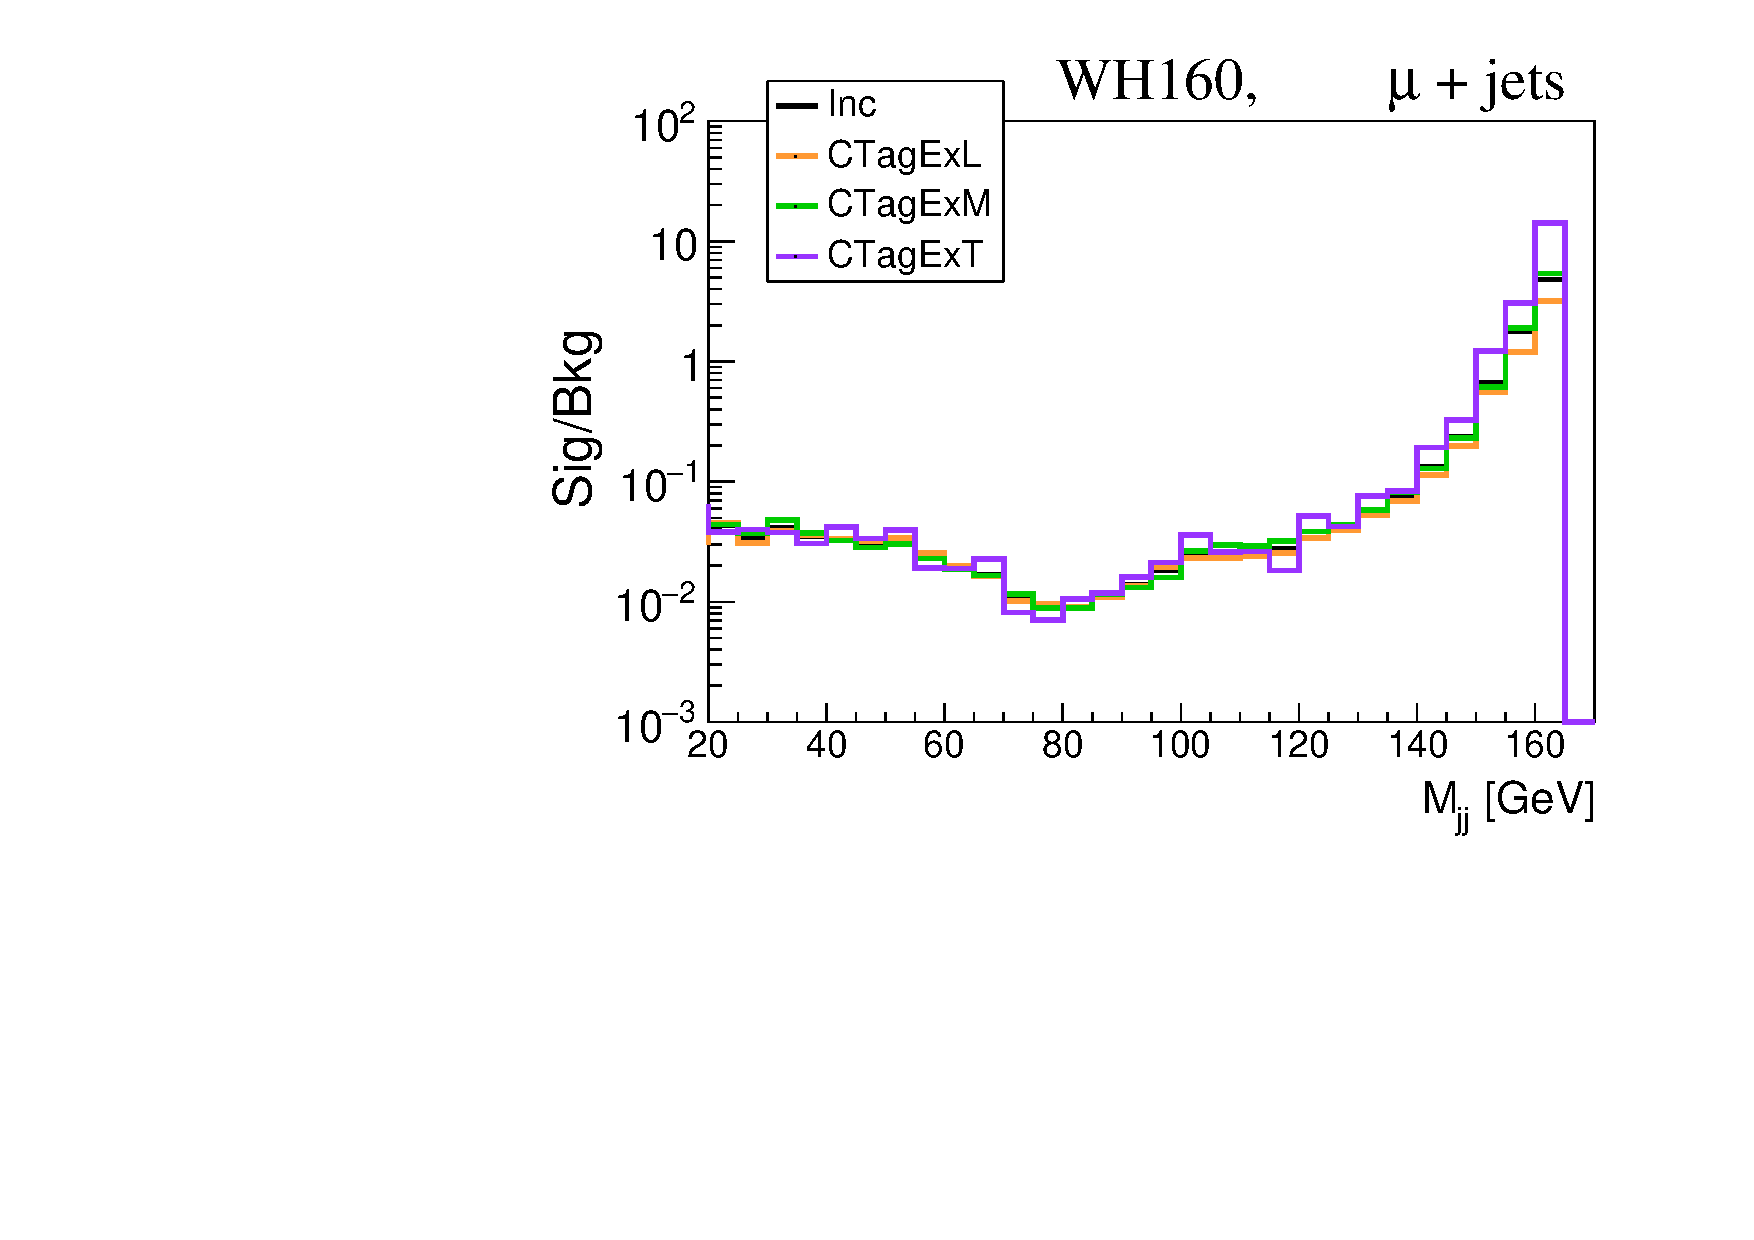
\includegraphics[width=0.45\linewidth]{Image/Muon/CTag/WH160_mu_ratioSB.pdf}}
\subfigure[]{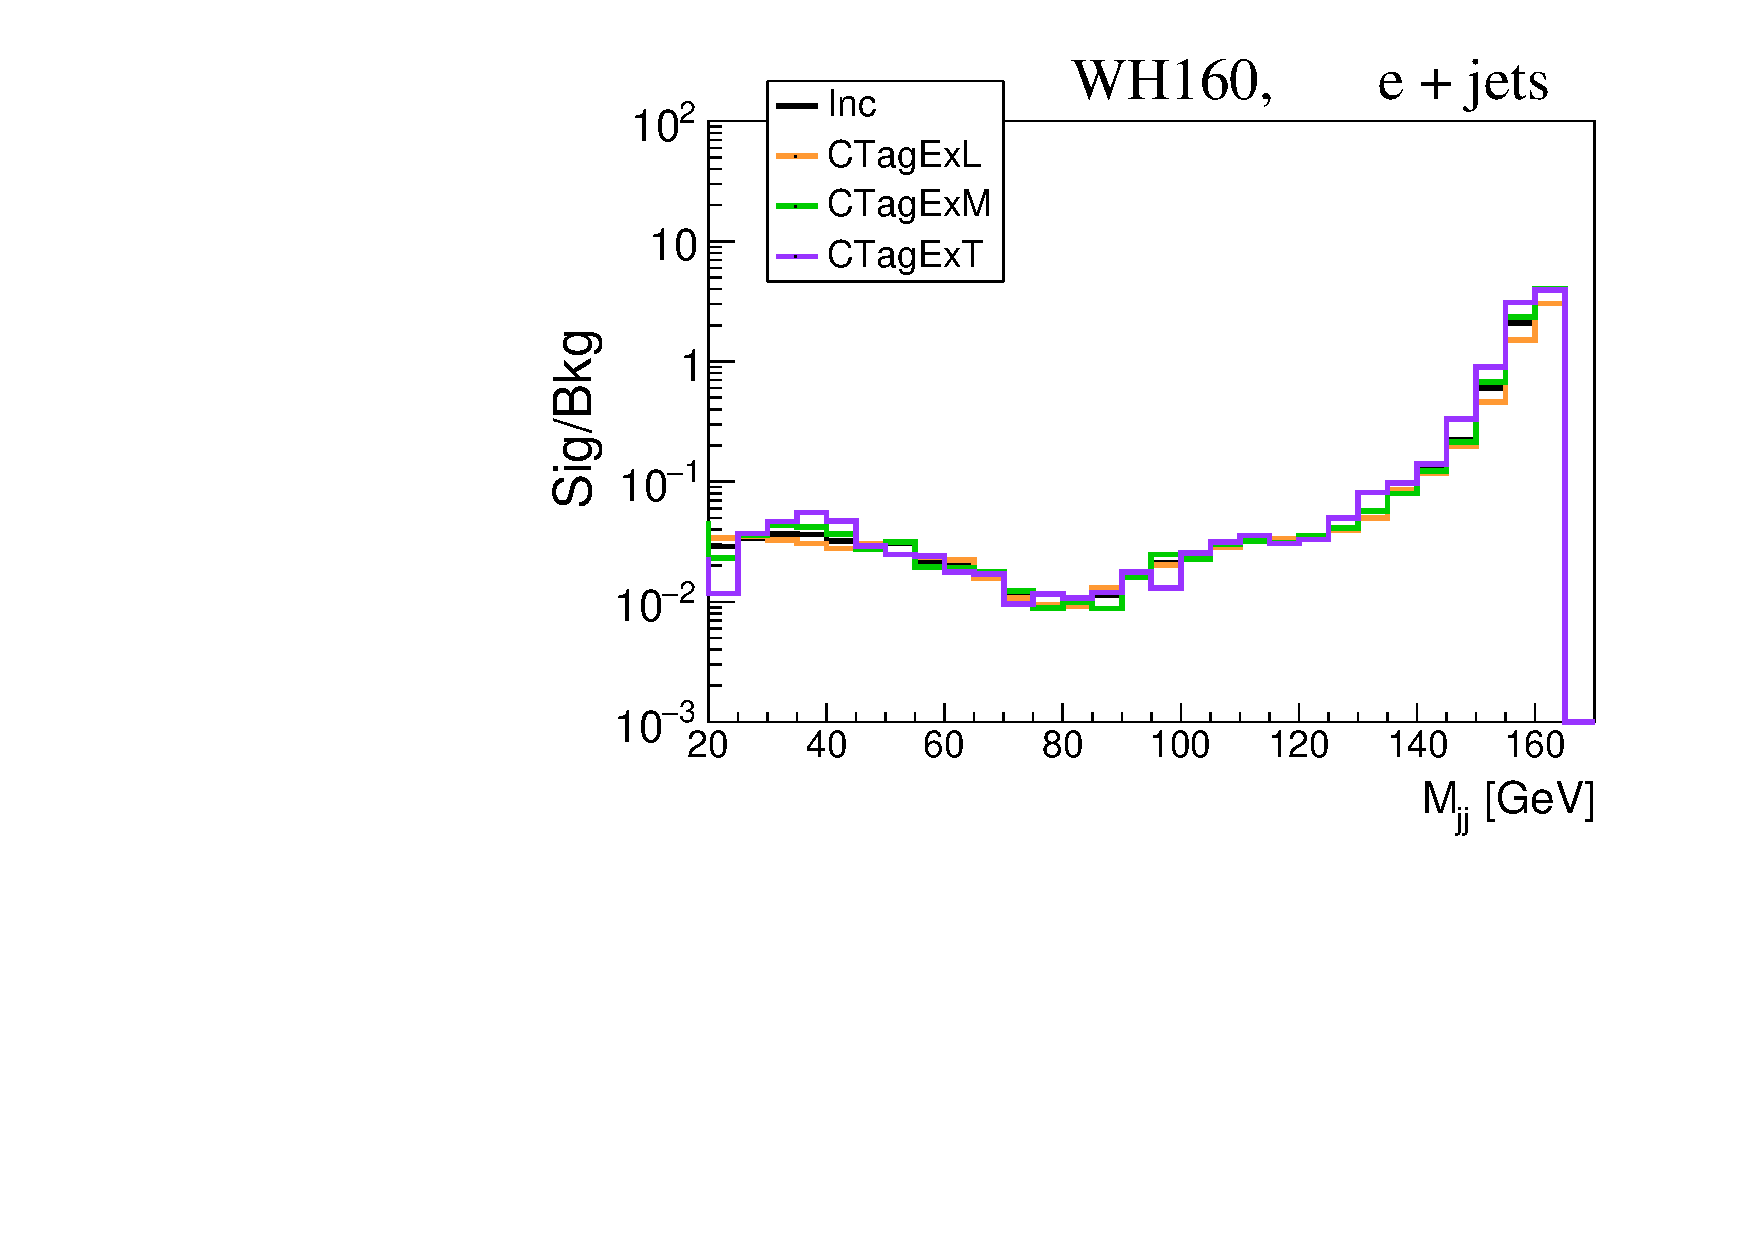
\includegraphics[width=0.45\linewidth]{Image/Electron/CTag/WH160_ele_ratioSB.pdf}}
\caption{Signal to background ratio for $m_{H^+}$ = 140, 150, 155, 160 GeV.}
\label{fig:ratioSB_2}
\end{figure}


\begin{figure}
\centering  
\subfigure[\mjj in loose category for muon channel]
{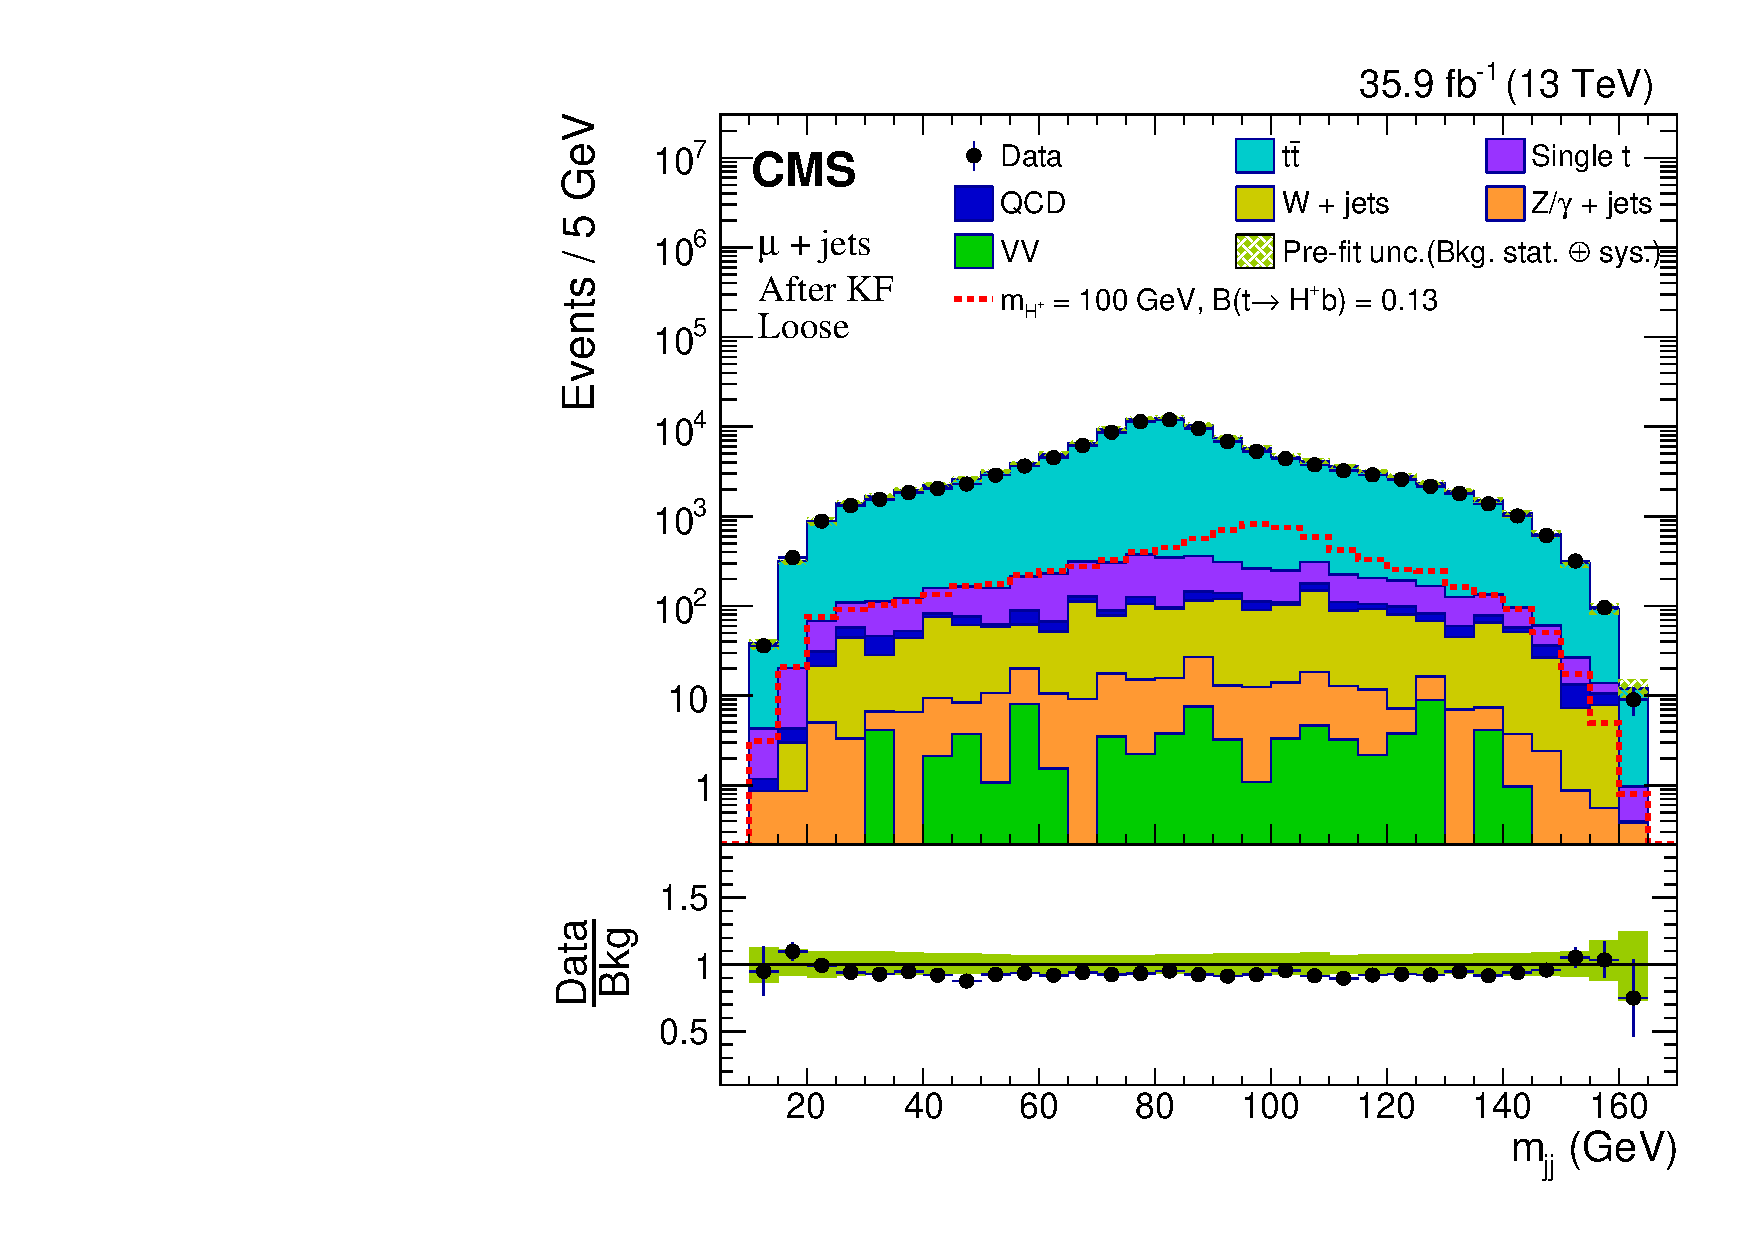
\includegraphics[width=0.40\linewidth]{Image/Muon/KinFit/mjj_kfit_CTagExL_muKinFit.pdf}}
\subfigure[\mjj in loose category for electron channel]
{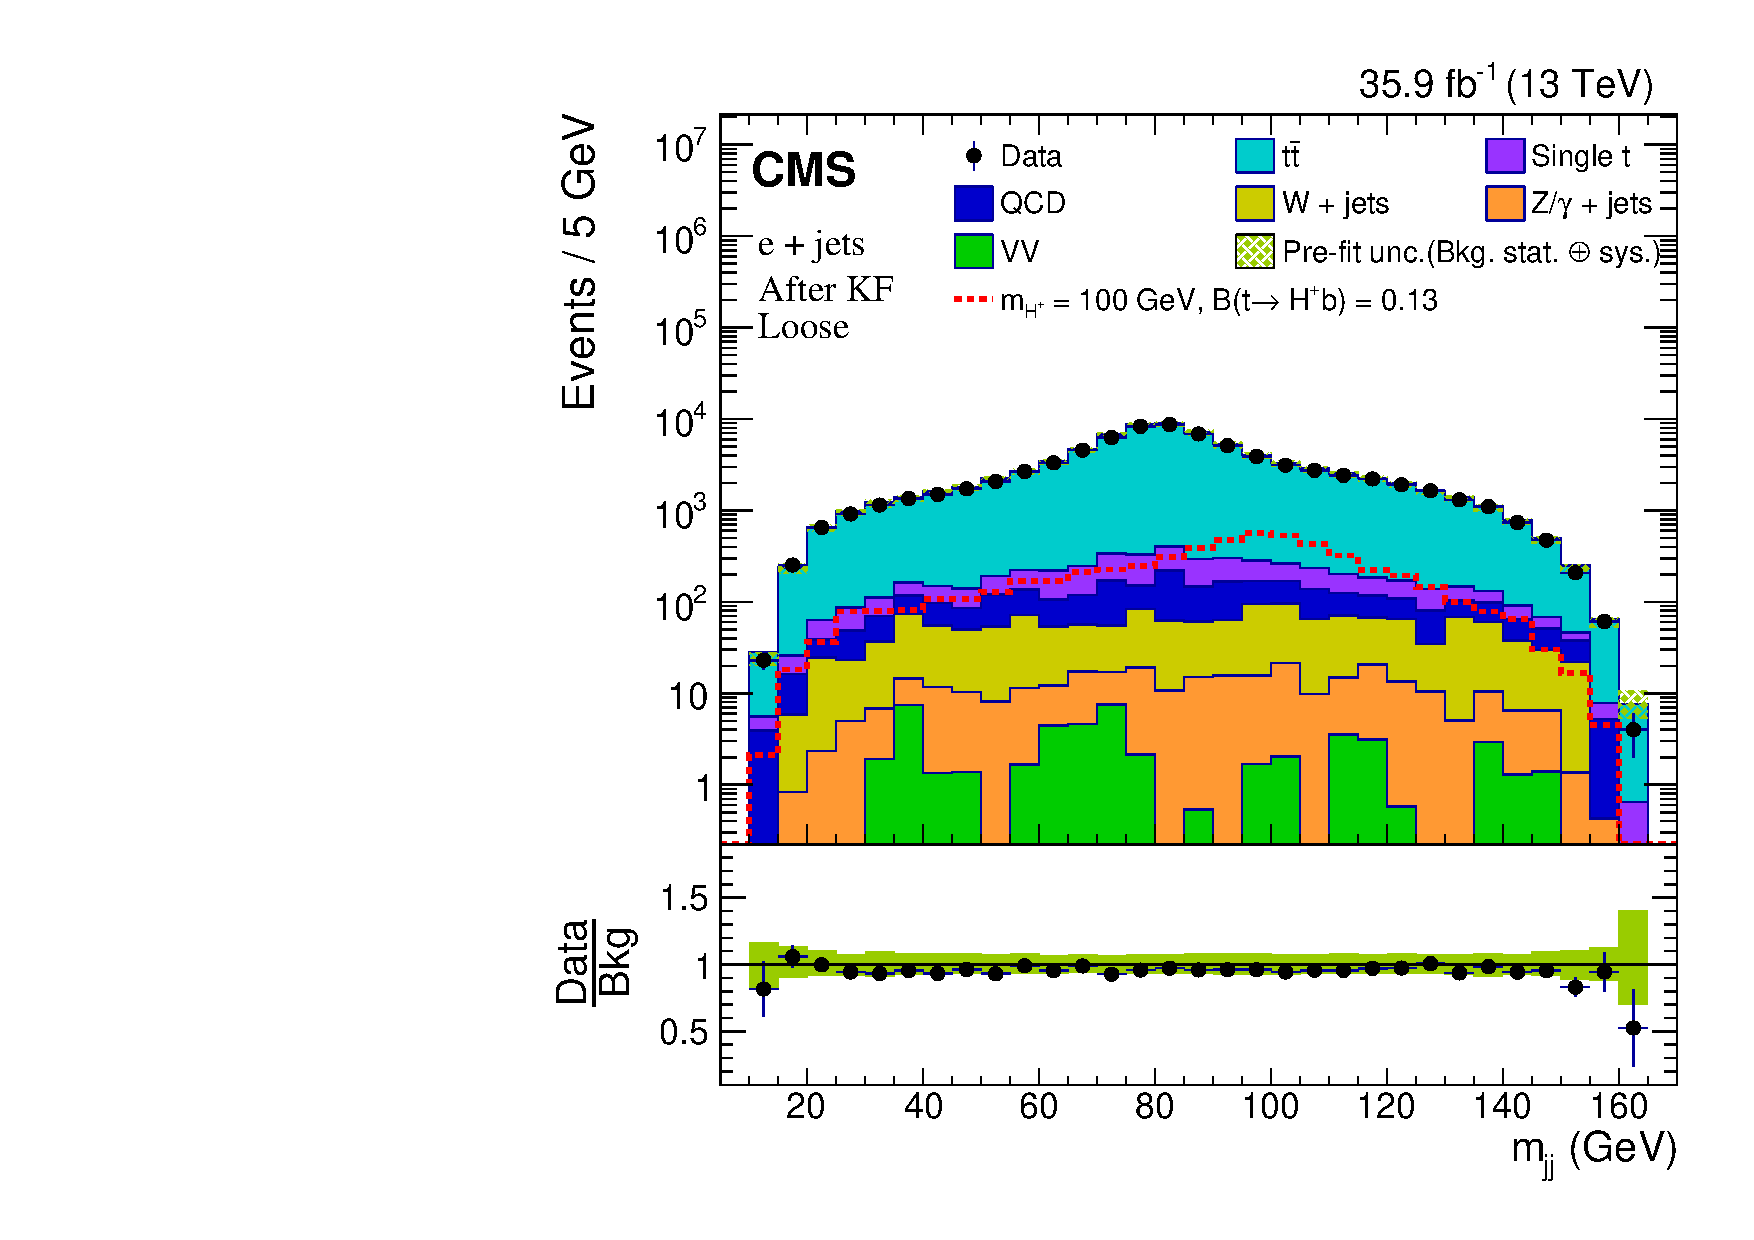
\includegraphics[width=0.40\linewidth]{Image/Electron/KinFit/mjj_kfit_CTagExL_eleKinFit.pdf}}
\vfil
\subfigure[\mjj in medium category for muon channel]
{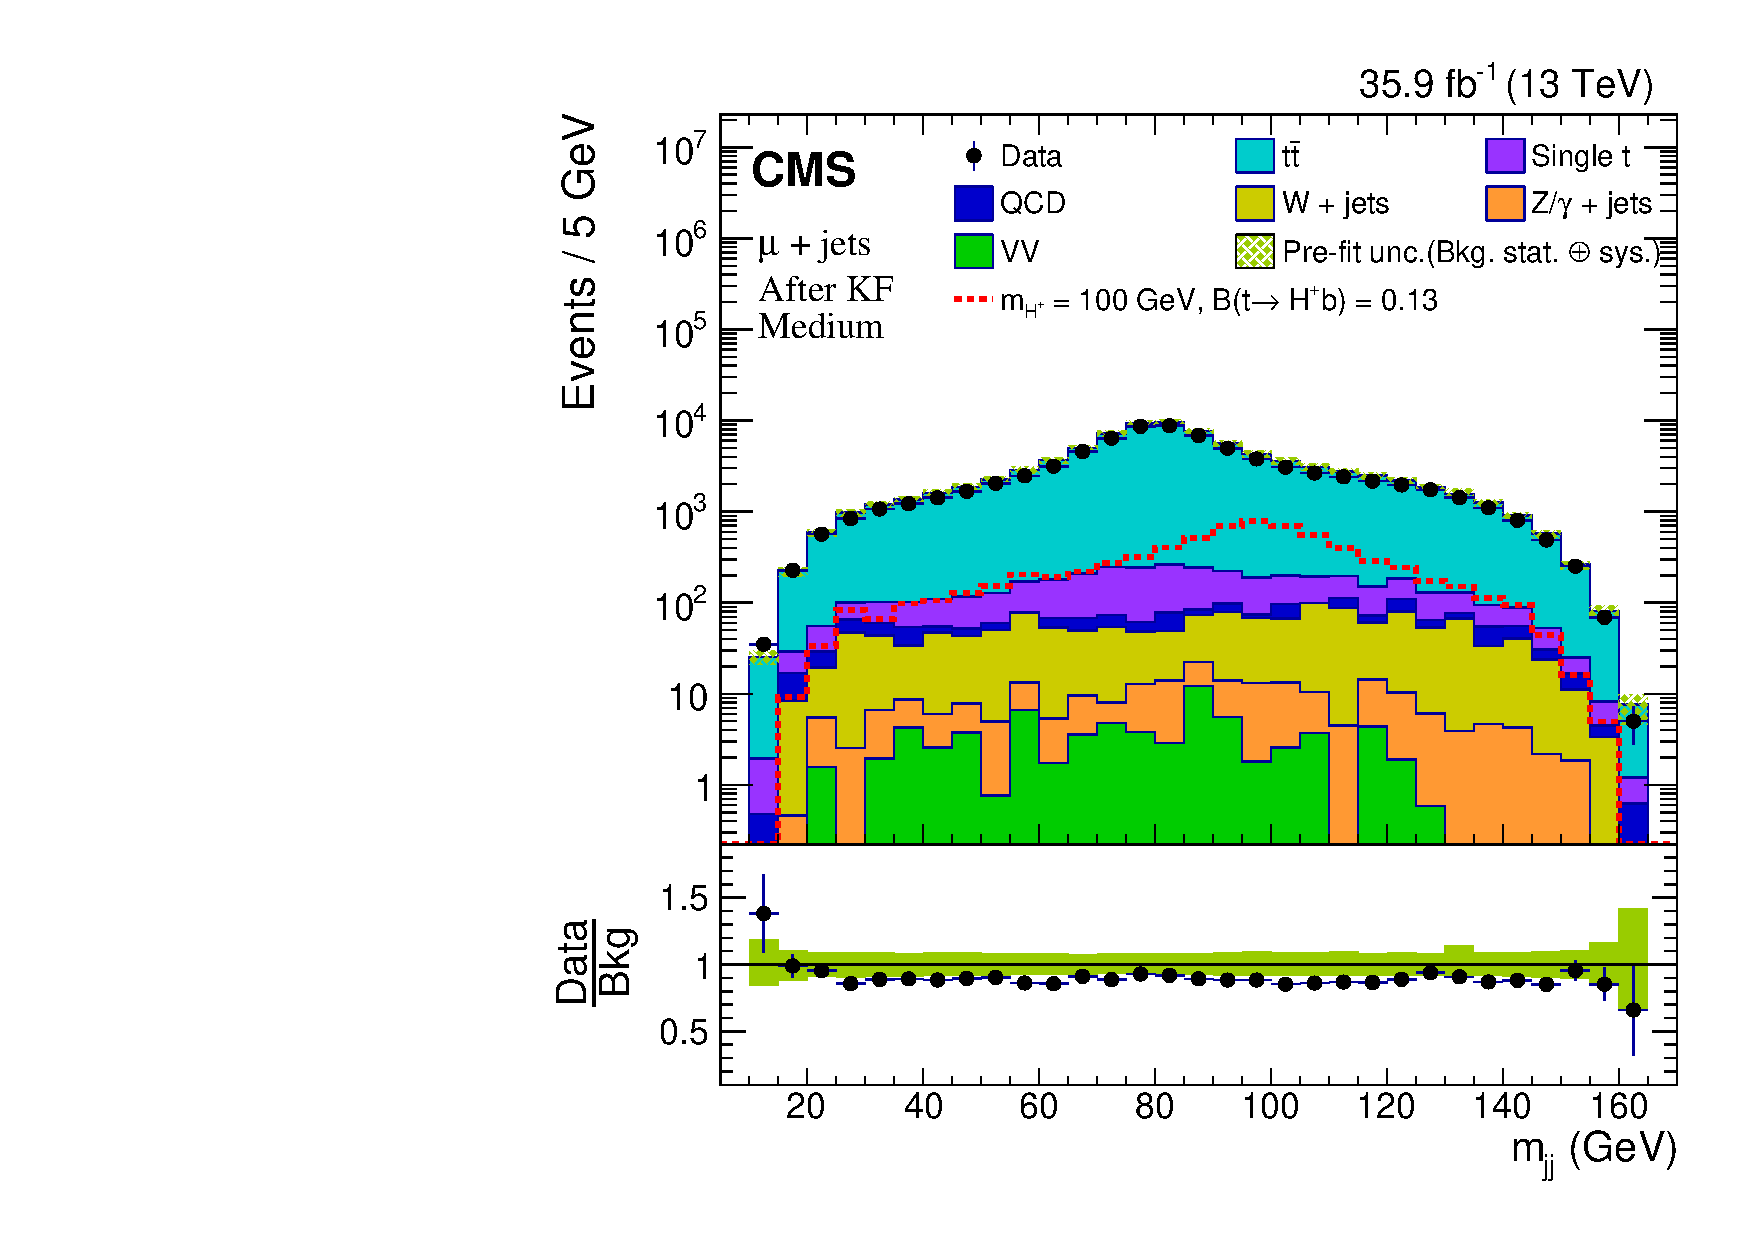
\includegraphics[width=0.40\linewidth]{Image/Muon/KinFit/mjj_kfit_CTagExM_muKinFit.pdf}}
\subfigure[\mjj in medium category for electron channel]
{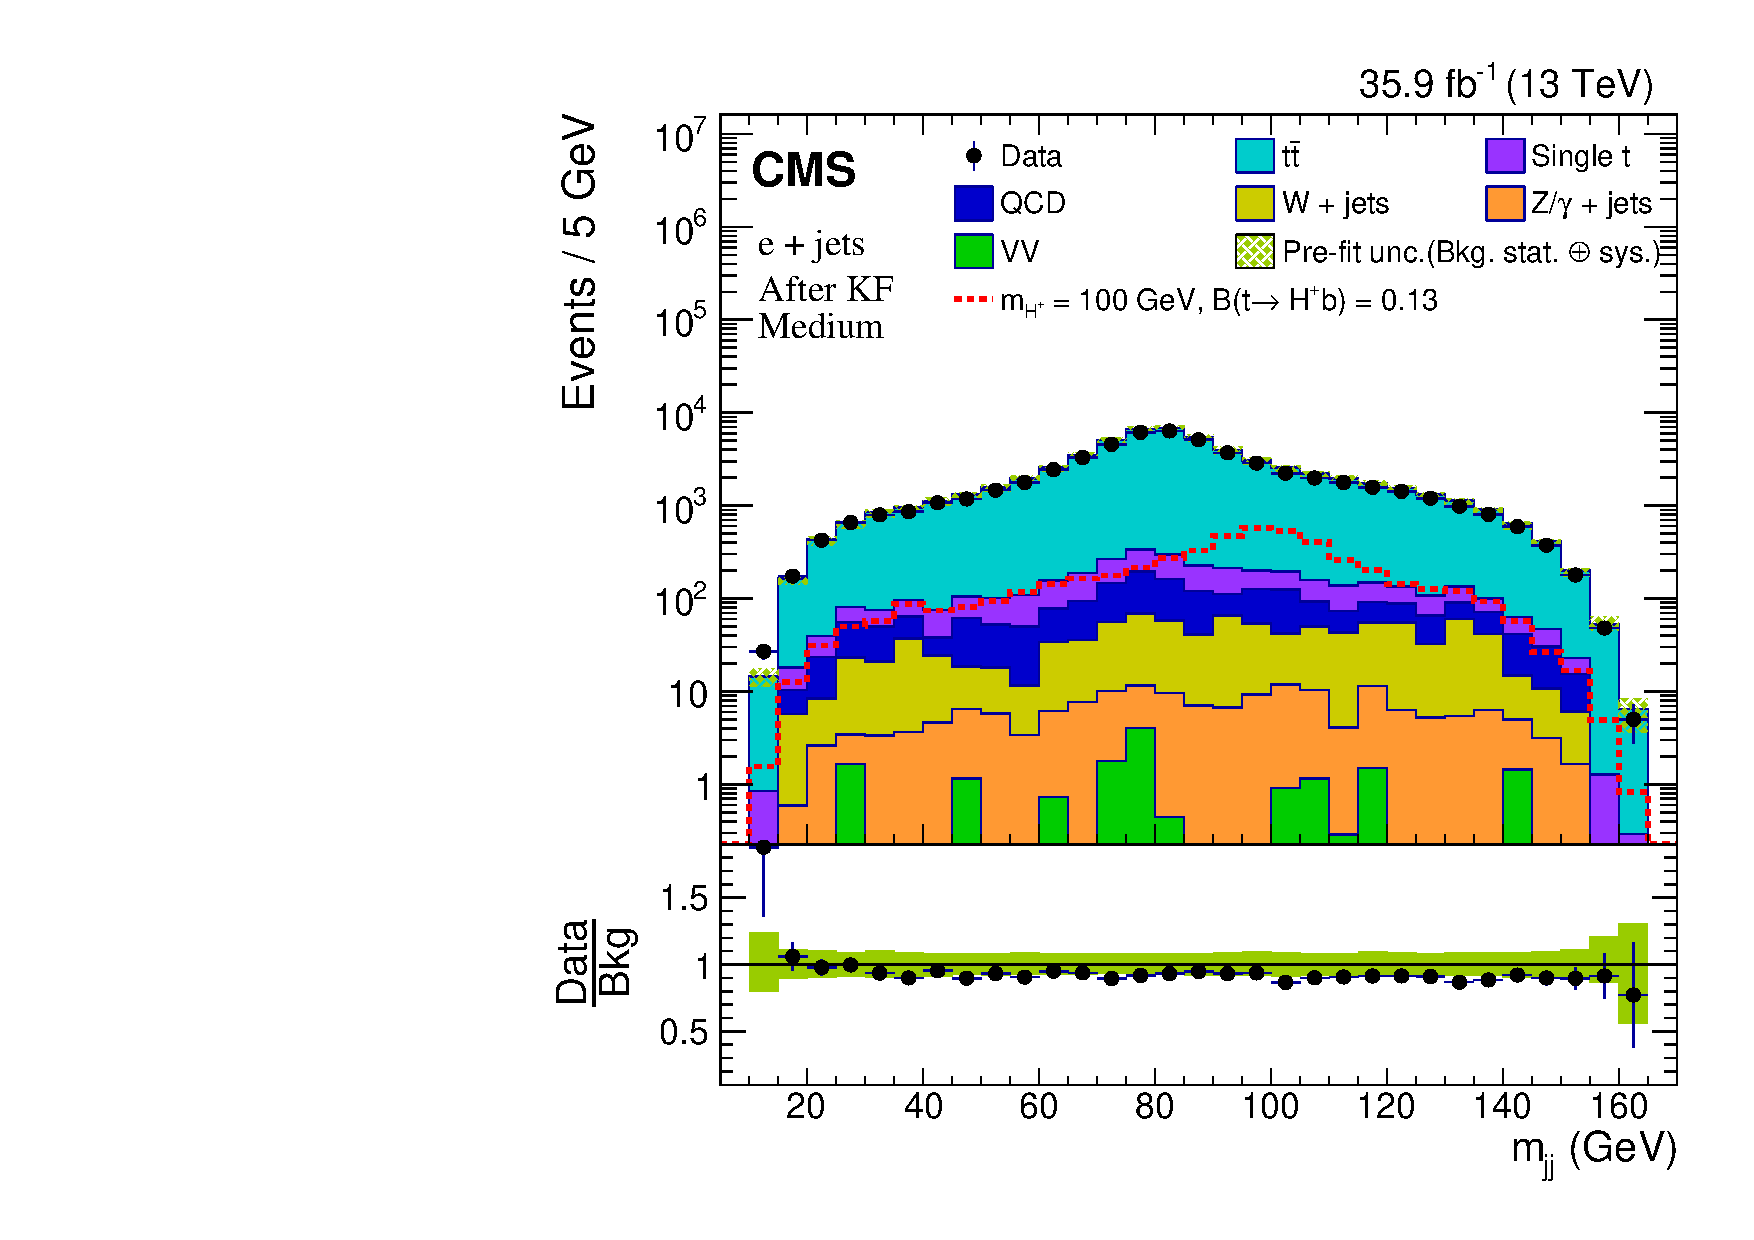
\includegraphics[width=0.40\linewidth]{Image/Electron/KinFit/mjj_kfit_CTagExM_eleKinFit.pdf}}
\vfil
\subfigure[\mjj in tight category for muon channel]
{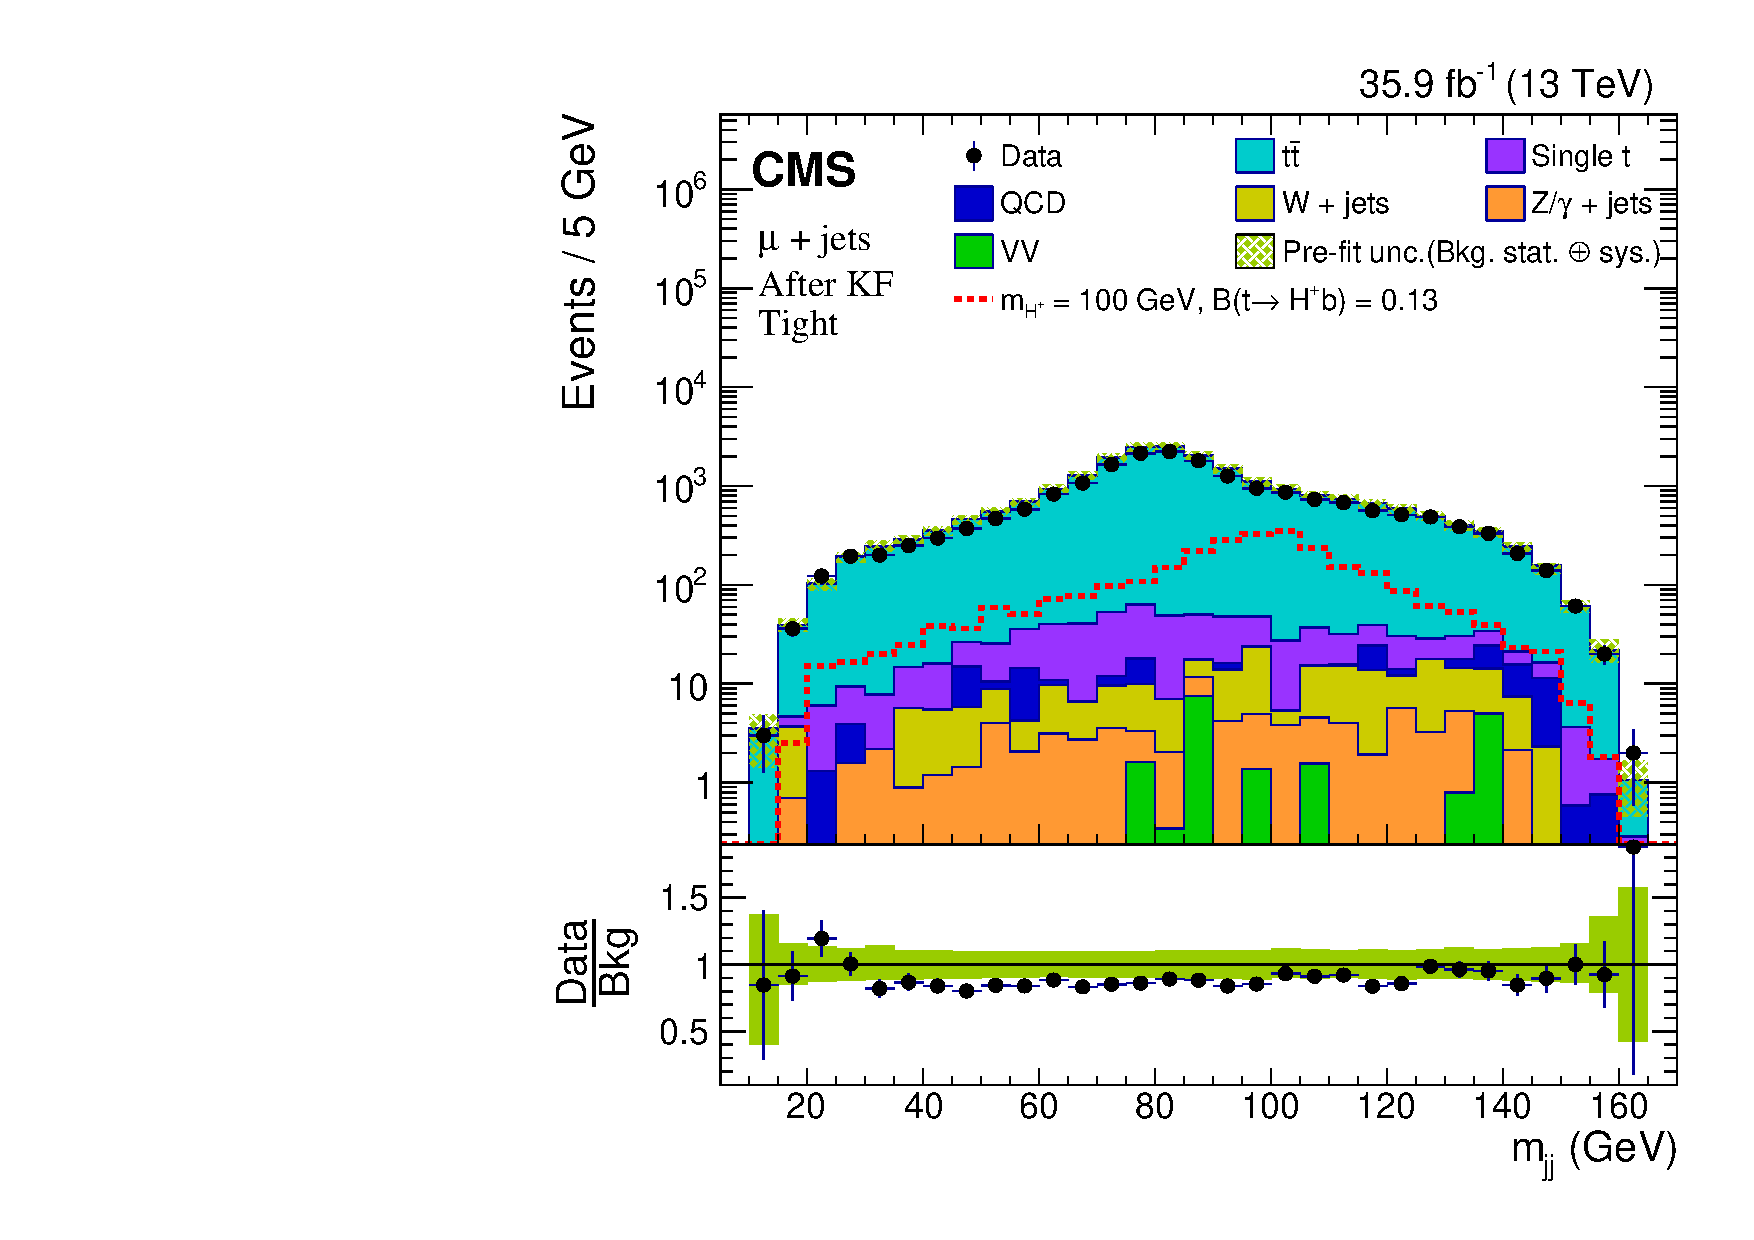
\includegraphics[width=0.40\linewidth]{Image/Muon/KinFit/mjj_kfit_CTagExT_muKinFit.pdf}}
\subfigure[\mjj in tight category for electron channel]
{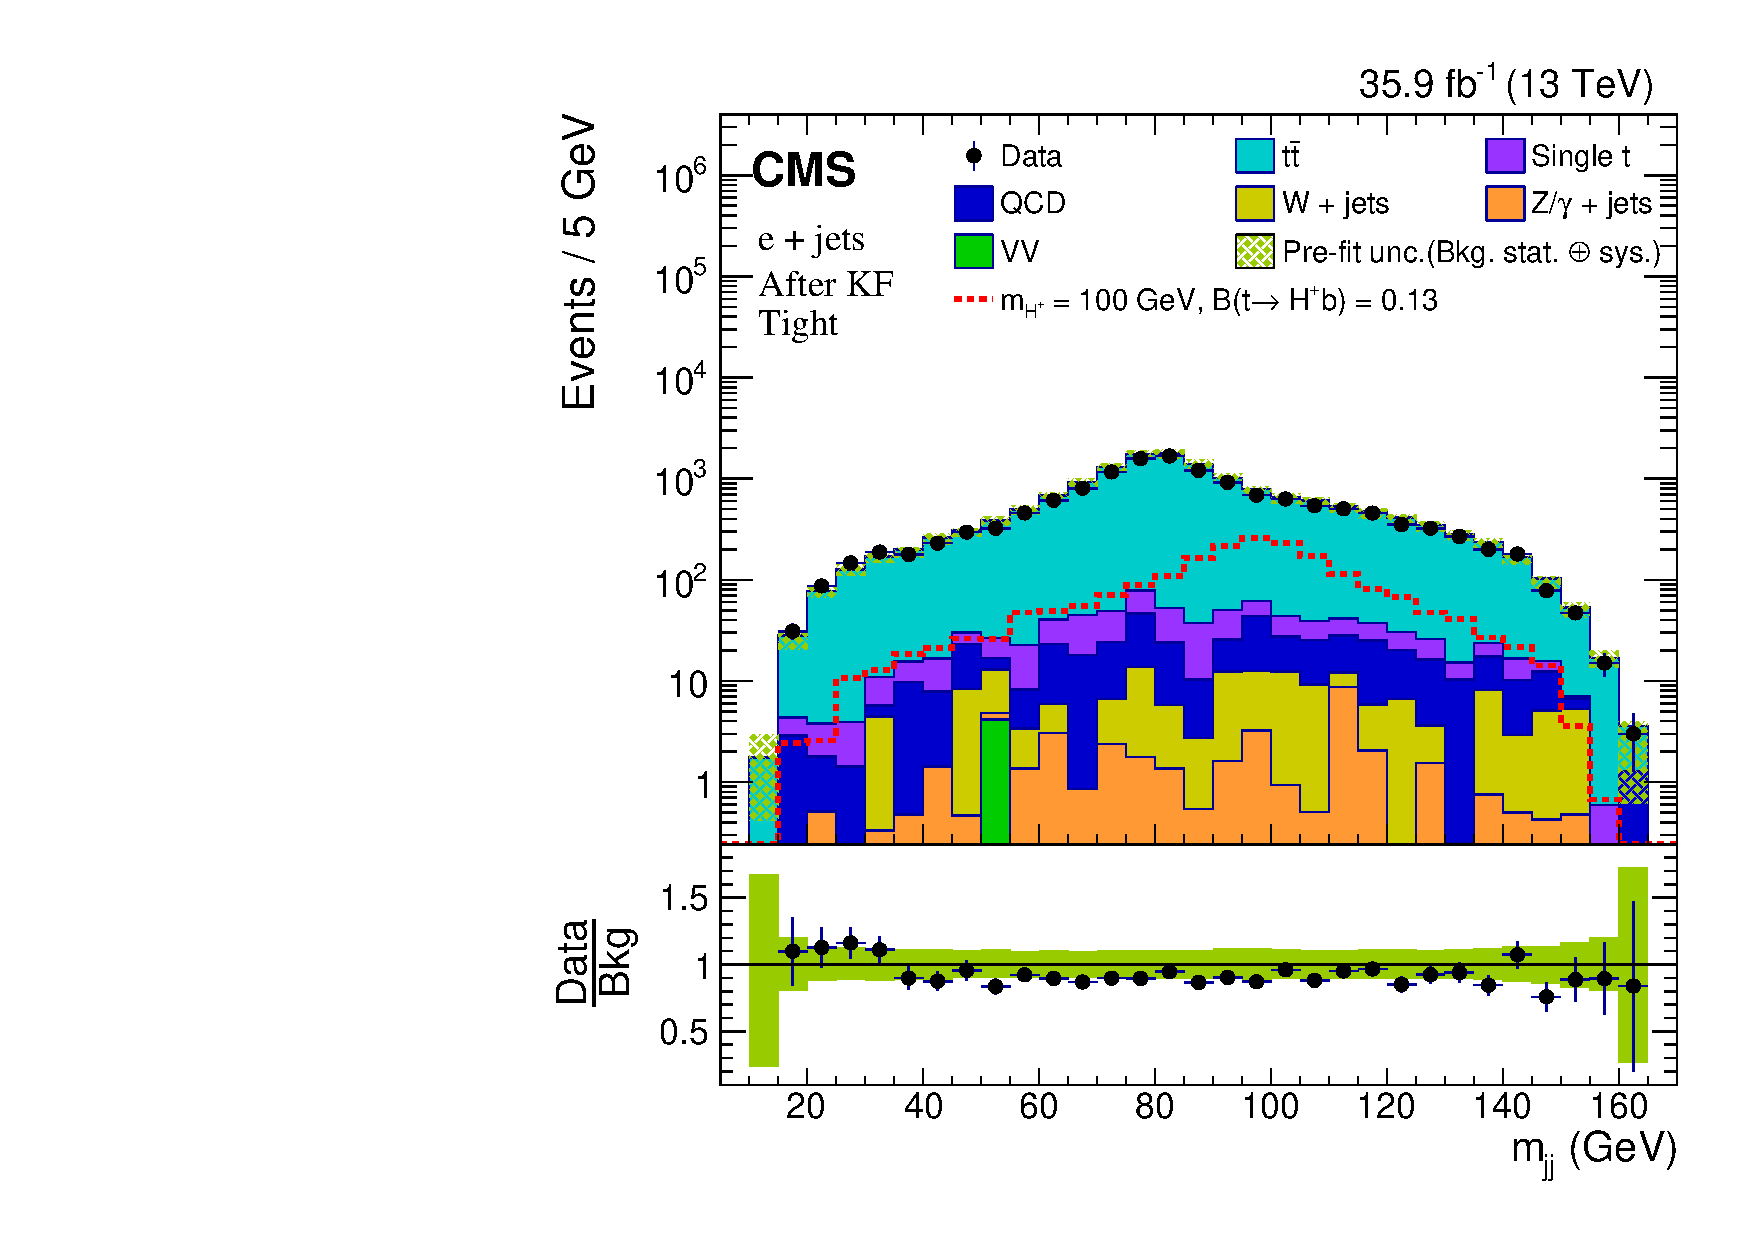
\includegraphics[width=0.40\linewidth]{Image/Electron/KinFit/mjj_kfit_CTagExT_eleKinFit.pdf}}
\caption{Distribution of \mjj from exclusive charm categories as described in
Sec.~\ref{ss:mjj_cTagEx} for \mujets and \ejets channel. The signal significance is different across different
exclusive categories.}
\label{fig:mjj_cTagEx}
\end{figure}
%\begin{landscape}
\begin{table}
\caption{Event yields with statistical and systematic uncertainties for signal 
    ($m_{H^+}$ = 80, 90, 100, 120, 140, 150, 155, 160 GeV) and background 
    processes in the \mujets and \ejets channel. Only statistical
    uncertainty in the QCD event is considered, as it is estimated from data.}  
\label{tab:eventYieldCTagEx}
\centering
\begin{adjustbox}{max width=\textwidth}
\begin{tabular}{cccccccc}
\hline 
\hline 
\multicolumn{1}{c}{{\bf{Process}}} & \multicolumn{2}{c}{{Exclusive loose category}} & \multicolumn{2}{c}{{Exclusive medium category}} & \multicolumn{2}{c}{{Exclusive tight category}} \\
& $N_{events} \pm stat \pm sys$ & $N_{events} \pm stat \pm sys$ & $N_{events} \pm stat \pm sys$ & $N_{events} \pm stat \pm sys$ & $N_{events} \pm stat \pm sys$ & $N_{events} \pm stat \pm sys$\\
 & $\mu$ + jets &  e + jets & $\mu$ + jets &  e + jets & $\mu$ + jets &  e + jets \\
\hline 
\hline 
$m_{\PSHp}=80$ \GeV & 7691 $\pm$ 77 $\pm$ 541 & 5427 $\pm$ 64 $\pm$ 371 & 6564 $\pm$ 74 $\pm$ 484 & 4695 $\pm$ 61 $\pm$ 363 & 2668 $\pm$ 45 $\pm$ 263 & 1855 $\pm$ 37 $\pm$ 172\\
$m_{\PSHp}=90$ \GeV & 7705 $\pm$ 77 $\pm$ 541 & 5616 $\pm$ 65 $\pm$ 397 & 6774 $\pm$ 74 $\pm$ 506 & 4856 $\pm$ 62 $\pm$ 377 & 2626 $\pm$ 44 $\pm$ 255 & 1865 $\pm$ 37 $\pm$ 184\\
$m_{\PSHp}=100$ \GeV & 7949 $\pm$ 78 $\pm$ 588 & 5548 $\pm$ 64 $\pm$ 398 & 7065 $\pm$ 76 $\pm$ 538 & 4945 $\pm$ 62 $\pm$ 349 & 2765 $\pm$ 45 $\pm$ 264 & 1997 $\pm$ 38 $\pm$ 195\\
$m_{\PSHp}=120$ \GeV & 7617 $\pm$ 76 $\pm$ 567 & 5360 $\pm$ 63 $\pm$ 390 & 6870 $\pm$ 75 $\pm$ 504 & 4780 $\pm$ 61 $\pm$ 355 & 2651 $\pm$ 44 $\pm$ 256 & 1962 $\pm$ 37 $\pm$ 188\\
$m_{\PSHp}=140$ \GeV & 6155 $\pm$ 69 $\pm$ 498 & 4365 $\pm$ 57 $\pm$ 359 & 5420 $\pm$ 66 $\pm$ 414 & 3838 $\pm$ 55 $\pm$ 301 & 2010 $\pm$ 38 $\pm$ 201 & 1497 $\pm$ 33 $\pm$ 150\\
$m_{\PSHp}=150$ \GeV & 4527 $\pm$ 59 $\pm$ 389 & 3227 $\pm$ 49 $\pm$ 278 & 3849 $\pm$ 56 $\pm$ 329 & 2795 $\pm$ 47 $\pm$ 242 & 1336 $\pm$ 31 $\pm$ 140 & 1027 $\pm$ 27 $\pm$ 117\\
$m_{\PSHp}=155$ \GeV & 3700 $\pm$ 54 $\pm$ 337 & 2559 $\pm$ 45 $\pm$ 242 & 2976 $\pm$ 50 $\pm$ 260 & 2231 $\pm$ 43 $\pm$ 215 & 1024 $\pm$ 28 $\pm$ 116 & 766 $\pm$ 24 $\pm$ 83\\
$m_{\PSHp}=160$ \GeV & 2777 $\pm$ 46 $\pm$ 267 & 2079 $\pm$ 39 $\pm$ 193 & 2371 $\pm$ 44 $\pm$ 228 & 1709 $\pm$ 37 $\pm$ 179 & 728 $\pm$ 23 $\pm$ 80 & 510 $\pm$ 19 $\pm$ 55\\
SM $t\bar{t}$ + jets & 107914 $\pm$ 201 $\pm$ 7633 & 75218 $\pm$ 166 $\pm$ 5400 & 81804 $\pm$ 184 $\pm$ 6571 & 56975 $\pm$ 152 $\pm$ 4638 & 21353 $\pm$ 90 $\pm$ 2112 & 14739 $\pm$ 73 $\pm$ 1486\\
Single ~t & 3105 $\pm$ 22 $\pm$ 254 & 2180 $\pm$ 18 $\pm$ 187 & 2294 $\pm$ 20 $\pm$ 212 & 1609 $\pm$ 17 $\pm$ 146 & 504 $\pm$ 9 $\pm$ 54 & 353 $\pm$ 8 $\pm$ 38\\
QCD multijet & 394 $\pm$ 78 $\pm$ 0 & 1539 $\pm$ 112 $\pm$ 0 & 399 $\pm$ 78 $\pm$ 0 & 1237 $\pm$ 116 $\pm$ 0 & 84 $\pm$ 40 $\pm$ 0 & 331 $\pm$ 57 $\pm$ 0\\
W + jets & 1661 $\pm$ 65 $\pm$ 277 & 1228 $\pm$ 55 $\pm$ 151 & 1240 $\pm$ 59 $\pm$ 238 & 819 $\pm$ 47 $\pm$ 110 & 168 $\pm$ 20 $\pm$ 45 & 123 $\pm$ 18 $\pm$ 17\\
$Z/\gamma$ + jets & 222 $\pm$ 13 $\pm$ 31 & 266 $\pm$ 11 $\pm$ 33 & 160 $\pm$ 9 $\pm$ 24 & 158 $\pm$ 9 $\pm$ 25 & 67 $\pm$ 6 $\pm$ 11 & 36 $\pm$ 5 $\pm$ 6\\
VV & 73 $\pm$ 14 $\pm$ 15 & 50 $\pm$ 11 $\pm$ 8 & 71 $\pm$ 14 $\pm$ 13 & 15 $\pm$ 5 $\pm$ 8 & 18 $\pm$ 7 $\pm$ 7 & 4 $\pm$ 4 $\pm$ 1\\
All background & 113370 $\pm$ 227 $\pm$ 8155 & 80480 $\pm$ 209 $\pm$ 5757 & 85968 $\pm$ 210 $\pm$ 7000 & 60811 $\pm$ 198 $\pm$ 4899 & 22195 $\pm$ 101 $\pm$ 2204 & 15586 $\pm$ 95 $\pm$ 1542\\
Data & 105474 $\pm$ 325 & 77244 $\pm$ 278 & 76807 $\pm$ 277 & 56051 $\pm$ 237 & 19437 $\pm$ 139 & 14179 $\pm$ 119 \\
\hline 
\end{tabular}
\end{adjustbox}
\end{table}
%\end{landscape}

\begin{table}
\caption{Systematic and statistical uncertainties in \%, from exclusive charm 
categories for muon (electron) channel. The "---" indicates that the 
corresponding uncertainties are not considered for the given process.}
\label{tab:sysCTagEx}
\centering
\begin{adjustbox}{max width=\textwidth}
\begin{tabular}{c  c c c c c c c c c c c c c cc}
\hline 
\hline 
Category & Process &{\rotatebox{90}{Luminosity}} & {\rotatebox{90}{Pileup} } & {\rotatebox{90}{Lepton }} & {\rotatebox{90}{JES + JER + \MET}} & { \rotatebox{90}{b \& c-jet tagging-1} }  & { \rotatebox{90}{b \& c-jet tagging-2} } & { \rotatebox{90}{b \& c-jet tagging-3}}& { \rotatebox{90}{Normalization}  }& {\rotatebox{90}{Statistical}  } & {\rotatebox{90}{top \pt } }  \\ 
\hline 
\hline 
$m_{\PSHp=80}$  \GeV & 2.5 (2.5) &  0.8 (1.0) &  3.0 (3.0) & 3.7 (3.1) &  1.1 (1.0) &  4.2 (4.2) &  4.0 (4.2) &  6.1 (6.1) & 1.0 (1.2) & 1.5 (1.9) \\ 
$m_{\PSHp=90}$  \GeV & 2.5 (2.5) &  0.5 (0.7) &  3.0 (3.0) & 3.7 (3.7) &  0.9 (0.9) &  4.2 (4.2) &  4.1 (4.2) &  6.1 (6.1) & 1.0 (1.1) & 1.4 (2.0) \\ 
$m_{\PSHp=100}$ \GeV & 2.5 (2.5) &  0.6 (1.1) &  3.0 (3.0) & 4.2 (3.5) &  0.9 (0.9) &  4.2 (4.3) &  4.3 (4.3) &  6.1 (6.1) & 1.0 (1.2) & 1.4 (1.8) \\ 
$m_{\PSHp=120}$ \GeV & 2.5 (2.5) &  0.6 (1.3) &  3.0 (3.0) & 4.0 (3.5) &  0.8 (1.0) &  4.2 (4.2) &  4.6 (4.6) &  6.1 (6.1) & 1.0 (1.2) & 1.4 (1.9) \\ 
$m_{\PSHp=140}$ \GeV & 2.5 (2.5) &  0.9 (1.3) &  3.0 (3.0) & 4.3 (4.6) &  0.8 (0.7) &  4.3 (4.3) &  5.2 (5.1) &  6.1 (6.1) & 1.1 (1.3) & 2.1 (2.4) \\ 
$m_{\PSHp=150}$ \GeV & 2.5 (2.5) &  0.7 (0.9) &  3.0 (3.0) & 4.6 (4.6) &  0.5 (0.8) &  4.6 (4.4) &  5.5 (5.6) &  6.1 (6.1) & 1.3 (1.5) & 2.6 (3.2) \\ 
$m_{\PSHp=155}$ \GeV & 2.5 (2.5) &  0.9 (0.8) &  3.0 (3.0) & 4.8 (5.6) &  0.7 (0.6) &  5.0 (4.9) &  5.8 (5.8) &  6.1 (6.1) & 1.5 (1.7) & 3.1 (3.5) \\ 
$m_{\PSHp=160}$ \GeV & 2.5 (2.5) &  0.5 (1.0) &  3.0 (3.0) & 5.7 (5.1) &  0.7 (0.5) &  5.0 (5.1) &  5.9 (5.7) &  6.1 (6.1) & 1.7 (1.9) & 3.2 (3.3) \\ 
\ttbar & 2.5 (2.5) &  0.9 (1.1) &  3.0 (3.0) & 3.6 (3.6) &  0.4 (0.4) &  4.5 (4.5) &  3.7 (3.7) &  6.1 (6.1) & 0.2 (0.2) & 1.5 (1.9) \\ 
Single \PQt  & 2.5 (2.5) &  0.6 (0.8) &  3.0 (3.0) & 4.9 (5.4) &  0.4 (0.4) &  5.0 (5.1) &  4.2 (4.2) &  5.0 (5.0) & 0.7 (0.8) & --- \\ 
\PW + jets & 2.5 (2.5) &  2.3 (0.4) &  3.0 (3.0) & 12.9 (6.9) &  0.1 (0.2) &  9.1 (8.9) &  5.0 (4.9) &  5.0 (5.0) & 3.9 (4.5) & --- \\ 
$\PZ/\PGg$ + jets & 2.5 (2.5) &  1.8 (2.4) &  3.0 (3.0) & 10.6 (8.4) &  0.0 (0.1) &  8.2 (7.7) &  4.2 (4.7) &  4.5 (4.5) & 5.7 (4.2) & --- \\ 
VV & 2.5 (2.5) &  1.5 (7.9) &  3.0 (3.0) & 18.6 (12.9) &  0.4 (0.7) &  4.8 (5.8) &  5.3 (3.9) &  4.0 (4.0) & 19.0 (22.0) & --- \\ 
QCD multijet & --- &  --- &  --- & --- &  --- &  --- &  --- &  10(10) & 19.9 (7.3) & --- \\ 
[\cmsTabSkip]
$m_{\PSHp=80}$  \GeV & 2.5 (2.5) &  0.6 (0.6) &  3.0 (3.0) & 2.8 (3.7) &  2.7 (2.8) &  5.1 (5.0) &  3.6 (3.5) &  6.1 (6.1) & 1.1 (1.3) & 1.6 (2.0) \\ 
$m_{\PSHp=90}$  \GeV & 2.5 (2.5) &  0.7 (0.6) &  3.0 (3.0) & 3.1 (3.8) &  2.7 (2.7) &  5.0 (5.0) &  3.6 (3.6) &  6.1 (6.1) & 1.1 (1.3) & 1.6 (2.2) \\ 
$m_{\PSHp=100}$ \GeV & 2.5 (2.5) &  0.4 (0.3) &  3.0 (3.0) & 3.5 (2.0) &  2.7 (2.7) &  5.0 (5.0) &  3.7 (3.7) &  6.1 (6.1) & 1.1 (1.3) & 1.6 (1.9) \\ 
$m_{\PSHp=120}$ \GeV & 2.5 (2.5) &  0.3 (0.7) &  3.0 (3.0) & 2.8 (3.0) &  2.7 (2.7) &  4.9 (4.9) &  3.9 (3.8) &  6.1 (6.1) & 1.1 (1.3) & 1.6 (2.0) \\ 
$m_{\PSHp=140}$ \GeV & 2.5 (2.5) &  0.4 (0.5) &  3.0 (3.0) & 2.9 (3.5) &  2.7 (2.6) &  5.0 (5.0) &  4.2 (4.1) &  6.1 (6.1) & 1.2 (1.4) & 2.2 (2.5) \\ 
$m_{\PSHp=150}$ \GeV & 2.5 (2.5) &  0.1 (0.6) &  3.0 (3.0) & 4.3 (4.3) &  2.5 (2.6) &  5.4 (5.5) &  4.4 (4.4) &  6.1 (6.1) & 1.5 (1.7) & 2.6 (3.4) \\ 
$m_{\PSHp=155}$ \GeV & 2.5 (2.5) &  0.1 (0.4) &  3.0 (3.0) & 4.4 (5.8) &  2.3 (2.4) &  5.5 (5.6) &  4.6 (4.6) &  6.1 (6.1) & 1.7 (1.9) & 3.2 (3.5) \\ 
$m_{\PSHp=160}$ \GeV & 2.5 (2.5) &  0.3 (0.4) &  3.0 (3.0) & 5.3 (6.8) &  2.2 (2.2) &  6.0 (6.0) &  4.9 (4.8) &  6.1 (6.1) & 1.9 (2.2) & 3.4 (3.7) \\ 
\ttbar & 2.5 (2.5) &  0.3 (0.4) &  3.0 (3.0) & 3.0 (3.0) &  1.5 (1.5) &  6.2 (6.2) &  3.4 (3.4) &  6.1 (6.1) & 0.2 (0.3) & 1.5 (2.0) \\ 
Single \PQt  & 2.5 (2.5) &  0.3 (0.1) &  3.0 (3.0) & 4.4 (4.1) &  1.2 (1.2) &  7.0 (7.0) &  3.8 (3.9) &  5.0 (5.0) & 0.9 (1.0) & --- \\ 
\PW + jets & 2.5 (2.5) &  2.9 (1.6) &  3.0 (3.0) & 14.4 (6.8) &  0.7 (0.7) &  11.5 (10.4) &  4.5 (4.8) &  5.0 (5.0) & 4.8 (5.7) & --- \\ 
$\PZ/\PGg$ + jets & 2.5 (2.5) &  0.7 (3.4) &  3.0 (3.0) & 9.0 (10.7) &  0.5 (0.4) &  11.0 (10.7) &  4.1 (4.1) &  4.5 (4.5) & 5.9 (5.9) & --- \\ 
VV & 2.5 (2.5) &  0.6 (4.4) &  3.0 (3.0) & 15.5 (49.2) &  1.5 (1.9) &  8.6 (8.6) &  5.3 (3.2) &  4.0 (4.0) & 20.4 (36.1) & --- \\ 
QCD multijet & --- &  --- &  --- & --- &  --- &  --- &  --- &  10(10) & 19.5 (9.4) & --- \\ 
[\cmsTabSkip]
$m_{\PSHp=80}$  \GeV & 2.5 (2.5) &  1.3 (1.3) &  3.0 (3.0) & 3.2 (1.5) &  5.7 (5.6) &  4.9 (4.8) &  5.3 (5.3) &  6.1 (6.1) & 1.7 (2.0) & 1.7 (1.8) \\ 
$m_{\PSHp=90}$  \GeV & 2.5 (2.5) &  0.8 (1.5) &  3.0 (3.0) & 3.0 (3.2) &  5.7 (5.6) &  5.0 (5.1) &  5.3 (5.2) &  6.1 (6.1) & 1.7 (2.0) & 1.4 (2.1) \\ 
$m_{\PSHp=100}$ \GeV & 2.5 (2.5) &  1.2 (1.3) &  3.0 (3.0) & 2.2 (3.0) &  5.6 (5.7) &  4.9 (5.0) &  5.4 (5.3) &  6.1 (6.1) & 1.6 (1.9) & 1.4 (1.8) \\ 
$m_{\PSHp=120}$ \GeV & 2.5 (2.5) &  1.0 (1.3) &  3.0 (3.0) & 2.6 (2.2) &  5.7 (5.7) &  4.9 (4.9) &  5.4 (5.3) &  6.1 (6.1) & 1.7 (1.9) & 1.4 (1.8) \\ 
$m_{\PSHp=140}$ \GeV & 2.5 (2.5) &  1.3 (1.3) &  3.0 (3.0) & 3.1 (3.1) &  6.0 (5.9) &  4.9 (5.0) &  5.4 (5.4) &  6.1 (6.1) & 1.9 (2.2) & 1.9 (2.3) \\ 
$m_{\PSHp=150}$ \GeV & 2.5 (2.5) &  1.4 (1.5) &  3.0 (3.0) & 3.6 (5.6) &  6.1 (6.0) &  5.0 (5.1) &  5.7 (5.8) &  6.1 (6.1) & 2.3 (2.6) & 2.8 (3.2) \\ 
$m_{\PSHp=155}$ \GeV & 2.5 (2.5) &  0.5 (0.6) &  3.0 (3.0) & 5.5 (4.6) &  5.7 (6.0) &  5.5 (5.2) &  5.9 (5.6) &  6.1 (6.1) & 2.7 (3.1) & 3.2 (3.6) \\ 
$m_{\PSHp=160}$ \GeV & 2.5 (2.5) &  0.1 (1.4) &  3.0 (3.0) & 4.4 (4.2) &  5.9 (5.7) &  5.7 (5.6) &  5.8 (5.9) &  6.1 (6.1) & 3.2 (3.7) & 4.2 (4.5) \\ 
\ttbar & 2.5 (2.5) &  0.9 (1.0) &  3.0 (3.0) & 2.7 (3.1) &  4.7 (4.8) &  6.3 (6.3) &  5.1 (5.1) &  6.1 (6.1) & 0.4 (0.5) & 1.4 (1.8) \\ 
Single \PQt  & 2.5 (2.5) &  0.4 (0.5) &  3.0 (3.0) & 4.3 (4.5) &  4.2 (4.4) &  6.9 (6.8) &  5.4 (5.5) &  5.0 (5.0) & 1.8 (2.1) & --- \\ 
\PW + jets & 2.5 (2.5) &  1.1 (2.8) &  3.0 (3.0) & 23.3 (3.4) &  4.4 (2.7) &  9.8 (11.3) &  6.8 (5.9) &  5.0 (5.0) & 12.2 (14.4) & --- \\ 
$\PZ/\PGg$ + jets & 2.5 (2.5) &  3.7 (2.7) &  3.0 (3.0) & 7.5 (10.3) &  0.9 (2.4) &  12.4 (9.2) &  4.6 (6.8) &  4.5 (4.5) & 9.1 (15.2) & --- \\ 
VV & 2.5 (2.5) &  2.3 (8.9) &  3.0 (3.0) & 36.1 (0.3) &  5.7 (7.4) &  5.4 (6.9) &  7.3 (2.3) &  4.0 (4.0) & 38.5 (100.0) & --- \\ 
QCD multijet & --- &  --- &  --- & --- &  --- &  --- &  --- &  10(10) & 47.3 (17.2) & --- \\ 

\hline 
\end{tabular}
\end{adjustbox}
\end{table}

The charm-tag scale factors are officially not available for exclusive event 
categories. Therefore, conservatively, the inclusive scale factors are used for 
exclusive event categories. However, one extra systematic uncertainty is 
considered for exclusive categories. The mean of inclusive c-tag weights 
(Eq.~\ref{eq:btagWt}) is calculated based on whether a jet is satisfying one of
the charm WP and not satisfying other charm WP (e.g. the jet satisfies loose 
and medium but not tight WP, as shown in Table~\ref{tab:extraNPL},~\ref{tab:extraNPM}). 
\begin{itemize}
\item {\bf{\verb|CMS_eff_ExL|}}: The ratio (max/min) of mean of inclusive c-tag weights from four
    combinations (yLyMyT, yLyMnT, yLnMyT, yLnMnT) is considered as one extra NP (profiled as
    lnN) for exclusive loose charm category.
\item {\bf{\verb|CMS_eff_ExM|}}: For exclusive medium charm category, the ratio (max/min) of
    event weights from two combinations (yMyT, yMnT) are considered as one extra NP
    (profiled as lnN).
\end{itemize}
The inclusive and exclusive event categories are same for tight charm working points, hence no
extra NP is considered.
\begin{table}
\begin{center}
\begin{tabular}{cccc}
\hline
\hline
{\bf{Loose WP}} & {\bf{Medium WP}} & {\bf{Tight WP}} & {\bf{Acronym}} \\
\hline
\hline
Y     & Y & Y & yLyMyT \\
Y     & Y & N & yLyMnT \\
Y     & N & Y & yLnMyT \\
Y     & N & N & yLnMnT  \\
\hline
\end{tabular}
\caption{Inclusive loose c-tag types. The acronym yLyMnT refers to the case where a jet
\label{tab:extraNPL}
satisfies loose and medium, but not tight WP.}
\end{center}
\end{table}
\begin{table}
\begin{center}
\begin{tabular}{ccc}
\hline
\hline
{\bf{Medium WP}} & {\bf{Tight WP}} & {\bf{Acronym}} \\
\hline
\hline
 Y & Y & yMyT \\
 Y & N & yMnT \\
\hline
\end{tabular}
\caption{Inclusive medium c-tag types.}
\label{tab:extraNPM}
\end{center}
\end{table}
The loose and medium c-tag event weight corresponding to Table~\ref{tab:extraNPL},
~\ref{tab:extraNPM} are shown in Figure~\ref{fig:extraNP} for both channels, for SM \ttbar +
jets sample. Similar event weights are found for signal MC samples.
\begin{figure}
\centering  
\subfigure[c-tag weight from SM \ttbar sample for $\mu$ + jets channel 
\label{subfig:extraNPmu}]
{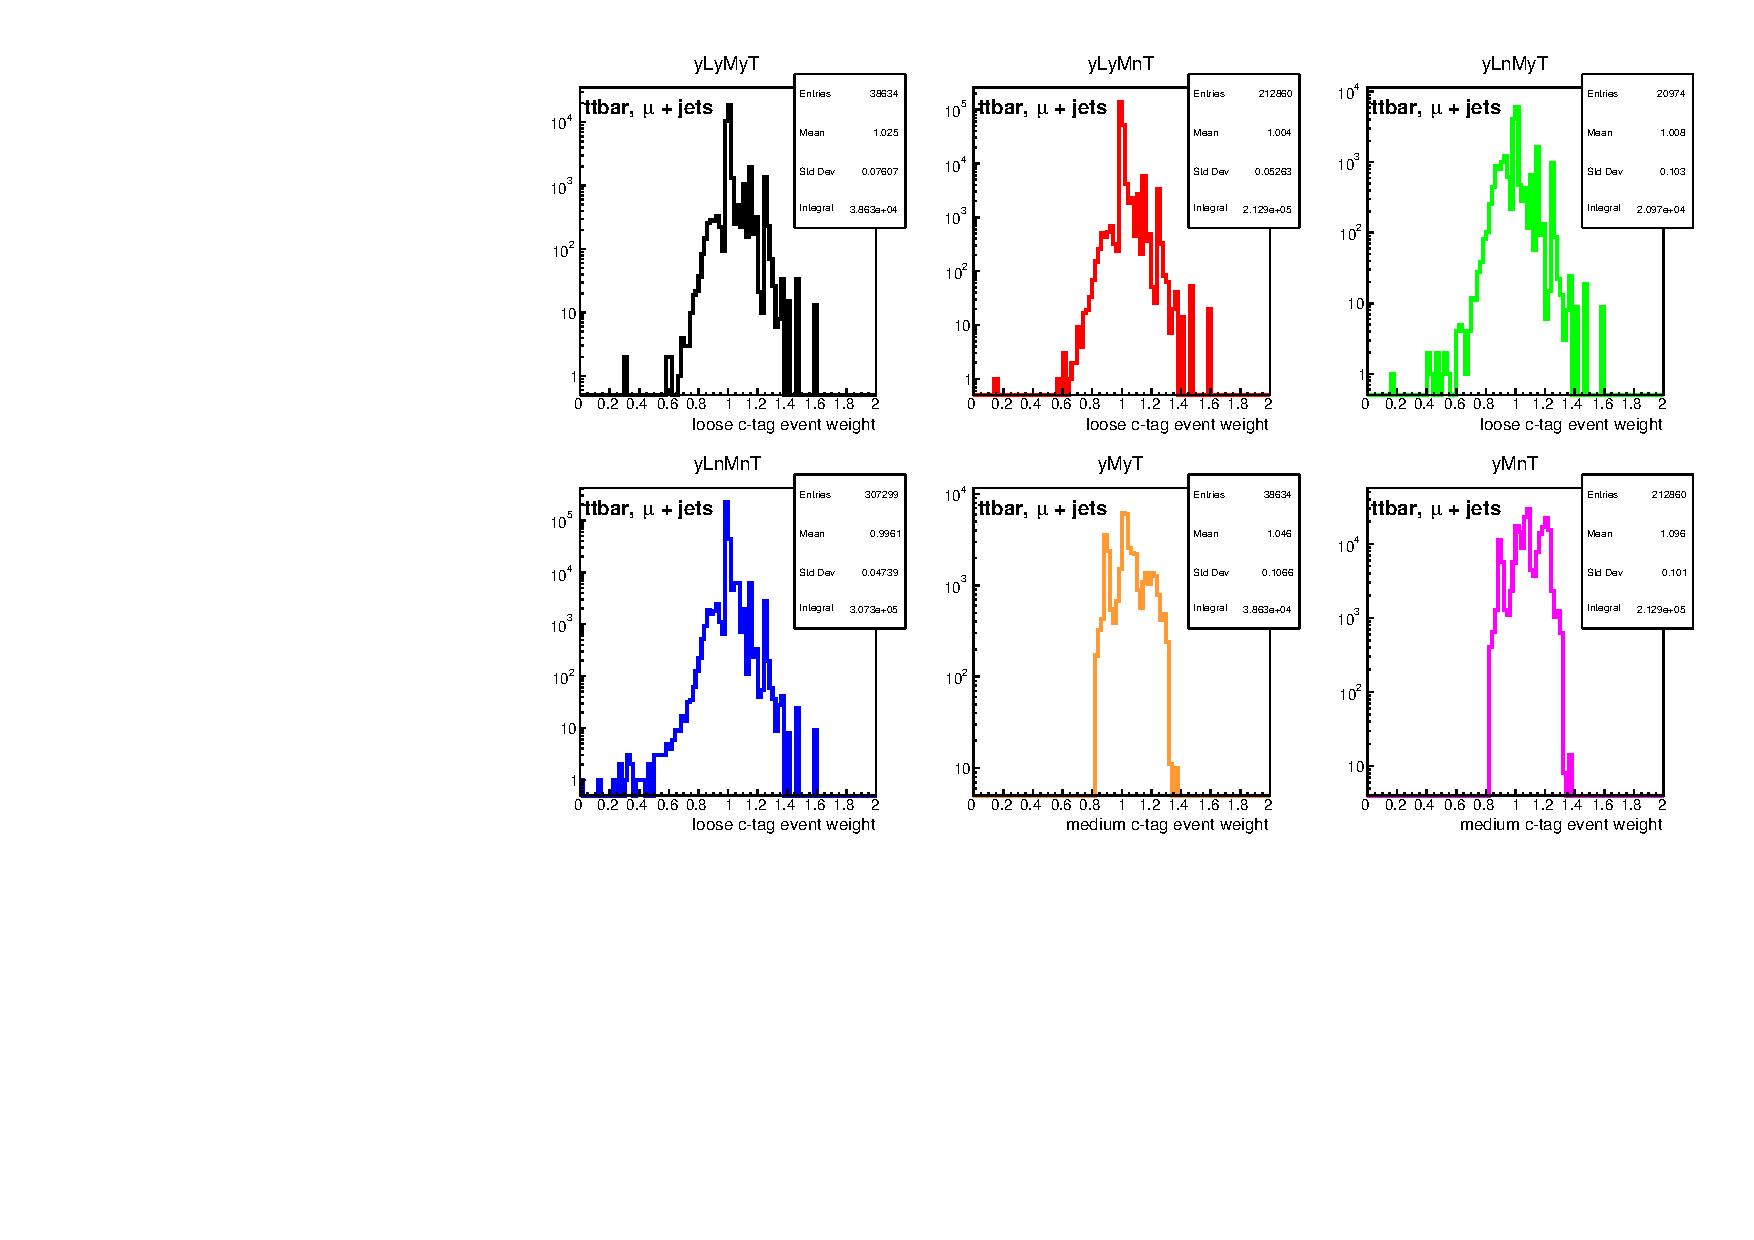
\includegraphics[width=0.90\linewidth]{Image/Muon/CTag/muExtraNP.pdf}}
\vfil
\subfigure[c-tag weight from SM \ttbar sample for $e$ + jets channel
\label{subfig:extraNPele}]
{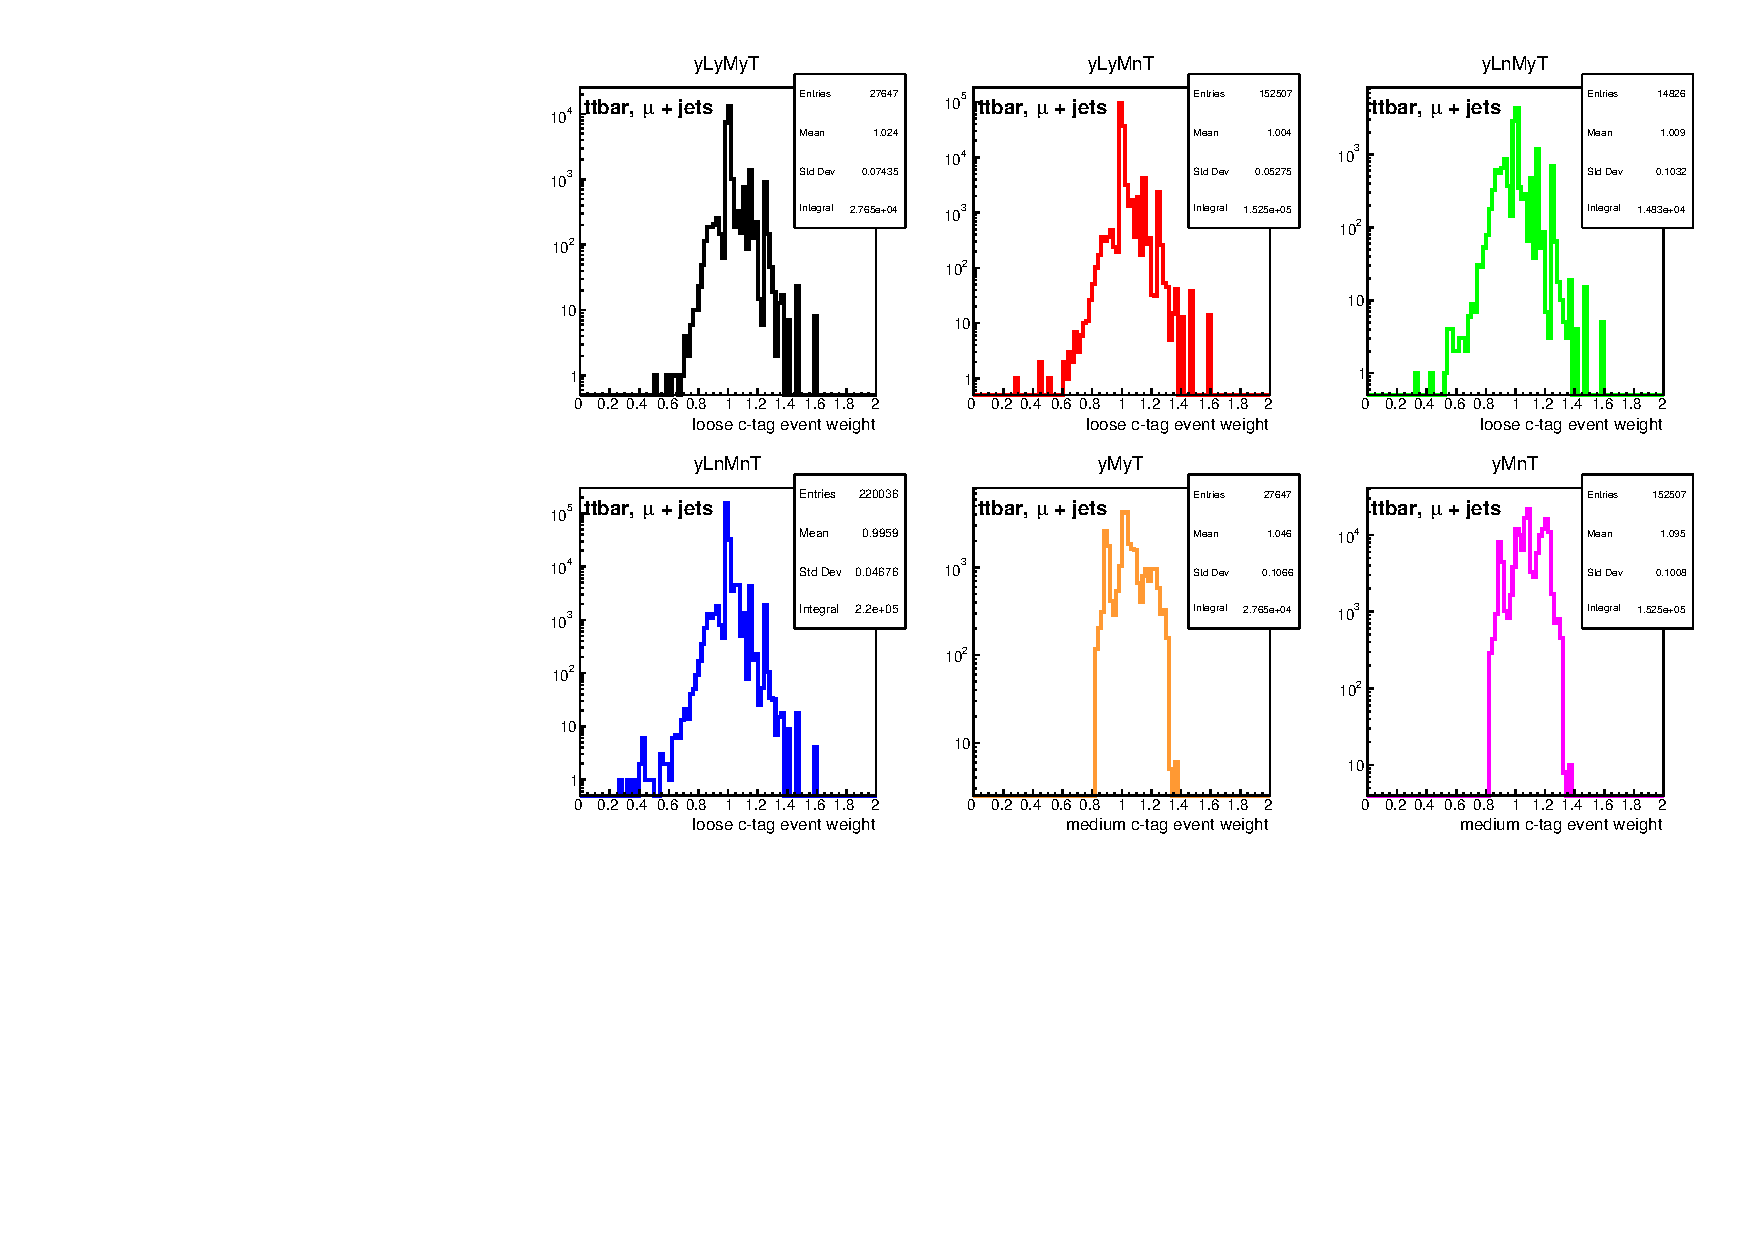
\includegraphics[width=0.90\linewidth]{Image/Electron/CTag/eleExtraNP.pdf}}
\caption{The c-tag event weight for different cases from SM \ttbar 
    sample. For exclusive loose charm category, the value of 
    $CMS\_eff\_ExL$ = 1.025/0.99 (1.024/0.99) for $\mu$ + jets 
    ($e$ + jets) channel. For exclusive medium charm category, the value of
    $CMS\_eff\_ExM$ = 1.096/1.046 (1.096/1.046) for $\mu$ + jets 
    ($e$ + jets) channel.}
\label{fig:extraNP}
\end{figure}


